\documentclass{book}
\usepackage[a4paper,top=2.5cm,bottom=2.5cm,left=2.5cm,right=2.5cm]{geometry}
\usepackage{makeidx}
\usepackage{natbib}
\usepackage{graphicx}
\usepackage{multicol}
\usepackage{float}
\usepackage{listings}
\usepackage{color}
\usepackage{ifthen}
\usepackage[table]{xcolor}
\usepackage{textcomp}
\usepackage{alltt}
\usepackage{ifpdf}
\ifpdf
\usepackage[pdftex,
            pagebackref=true,
            colorlinks=true,
            linkcolor=blue,
            unicode
           ]{hyperref}
\else
\usepackage[ps2pdf,
            pagebackref=true,
            colorlinks=true,
            linkcolor=blue,
            unicode
           ]{hyperref}
\usepackage{pspicture}
\fi
\usepackage[utf8]{inputenc}
\usepackage{mathptmx}
\usepackage[scaled=.90]{helvet}
\usepackage{courier}
\usepackage{sectsty}
\usepackage{amssymb}
\usepackage[titles]{tocloft}
\usepackage{doxygen}
\lstset{language=C++,inputencoding=utf8,basicstyle=\footnotesize,breaklines=true,breakatwhitespace=true,tabsize=8,numbers=left }
\makeindex
\setcounter{tocdepth}{3}
\renewcommand{\footrulewidth}{0.4pt}
\renewcommand{\familydefault}{\sfdefault}
\hfuzz=15pt
\setlength{\emergencystretch}{15pt}
\hbadness=750
\tolerance=750
\begin{document}
\hypersetup{pageanchor=false,citecolor=blue}
\begin{titlepage}
\vspace*{7cm}
\begin{center}
{\Large I\-T\-K\-Multigrid\-Anisotropic\-Diffusion \\[1ex]\large 1.\-0.\-0 }\\
\vspace*{1cm}
{\large Generated by Doxygen 1.8.1.2}\\
\vspace*{0.5cm}
{\small Fri Sep 5 2014 09:34:51}\\
\end{center}
\end{titlepage}
\clearemptydoublepage
\pagenumbering{roman}
\tableofcontents
\clearemptydoublepage
\pagenumbering{arabic}
\hypersetup{pageanchor=true,citecolor=blue}
\chapter{Class Index}
\section{Class Hierarchy}
This inheritance list is sorted roughly, but not completely, alphabetically\-:\begin{DoxyCompactList}
\item \contentsline{section}{itk\-:\-:mad\-:\-:Coarse\-Grid\-Operators\-Generator$<$ V\-Dimension $>$}{\pageref{classitk_1_1mad_1_1_coarse_grid_operators_generator}}{}
\item \contentsline{section}{itk\-:\-:mad\-:\-:Direct\-Solver$<$ V\-Dimension $>$}{\pageref{classitk_1_1mad_1_1_direct_solver}}{}
\item \contentsline{section}{itk\-:\-:mad\-:\-:Grids\-Hierarchy$<$ V\-Dimension $>$\-:\-:Grid}{\pageref{structitk_1_1mad_1_1_grids_hierarchy_1_1_grid}}{}
\item \contentsline{section}{itk\-:\-:mad\-:\-:Grids\-Hierarchy$<$ V\-Dimension $>$}{\pageref{classitk_1_1mad_1_1_grids_hierarchy}}{}
\item \contentsline{section}{Image}{\pageref{class_image}}{}
\begin{DoxyCompactList}
\item \contentsline{section}{itk\-:\-:mad\-:\-:Stencil\-Image$<$ T\-Pixel\-Type, V\-Dimension $>$}{\pageref{classitk_1_1mad_1_1_stencil_image}}{}
\end{DoxyCompactList}
\item \contentsline{section}{Image\-To\-Image\-Filter}{\pageref{class_image_to_image_filter}}{}
\begin{DoxyCompactList}
\item \contentsline{section}{itk\-:\-:Multigrid\-Anisotropic\-Diffusion\-Image\-Filter$<$ T\-Input\-Image, T\-Output\-Image, T\-Smoother\-Type $>$}{\pageref{classitk_1_1_multigrid_anisotropic_diffusion_image_filter}}{}
\item \contentsline{section}{itk\-:\-:V\-E\-D\-Multigrid\-Image\-Filter$<$ T\-Input\-Image, T\-Output\-Image, T\-Smoother\-Type $>$}{\pageref{classitk_1_1_v_e_d_multigrid_image_filter}}{}
\end{DoxyCompactList}
\item \contentsline{section}{itk\-:\-:mad\-:\-:Inter\-Grid\-Operators$<$ V\-Dimension $>$}{\pageref{classitk_1_1mad_1_1_inter_grid_operators}}{}
\item \contentsline{section}{itk\-:\-:mad\-:\-:Multigrid\-Smoother$<$ V\-Dimension $>$}{\pageref{classitk_1_1mad_1_1_multigrid_smoother}}{}
\begin{DoxyCompactList}
\item \contentsline{section}{itk\-:\-:mad\-:\-:Multigrid\-Gauss\-Seidel\-Smoother$<$ V\-Dimension $>$}{\pageref{classitk_1_1mad_1_1_multigrid_gauss_seidel_smoother}}{}
\item \contentsline{section}{itk\-:\-:mad\-:\-:Multigrid\-Weighted\-Jacobi\-Smoother$<$ V\-Dimension $>$}{\pageref{classitk_1_1mad_1_1_multigrid_weighted_jacobi_smoother}}{}
\end{DoxyCompactList}
\end{DoxyCompactList}

\chapter{Class Index}
\section{Class List}
Here are the classes, structs, unions and interfaces with brief descriptions\-:\begin{DoxyCompactList}
\item\contentsline{section}{\hyperlink{classitk_1_1mad_1_1_coarse_grid_operators_generator}{itk\-::mad\-::\-Coarse\-Grid\-Operators\-Generator$<$ V\-Dimension $>$} \\*Implementation of the two main generating rules for coarse operators\-: D\-C\-A for Geometric M\-G, and G\-C\-A for algebraic M\-G }{\pageref{classitk_1_1mad_1_1_coarse_grid_operators_generator}}{}
\item\contentsline{section}{\hyperlink{classitk_1_1mad_1_1_direct_solver}{itk\-::mad\-::\-Direct\-Solver$<$ V\-Dimension $>$} \\*Implementation of a direct solver to be used on the coarsest grid for problem }{\pageref{classitk_1_1mad_1_1_direct_solver}}{}
\item\contentsline{section}{\hyperlink{structitk_1_1mad_1_1_grids_hierarchy_1_1_grid}{itk\-::mad\-::\-Grids\-Hierarchy$<$ V\-Dimension $>$\-::\-Grid} }{\pageref{structitk_1_1mad_1_1_grids_hierarchy_1_1_grid}}{}
\item\contentsline{section}{\hyperlink{classitk_1_1mad_1_1_grids_hierarchy}{itk\-::mad\-::\-Grids\-Hierarchy$<$ V\-Dimension $>$} \\*Class which creates and holds a hierarchy of grids to be used by itk\-Multigrid\-Anisotropic\-Diffusion. It contains informations about each level's grid\-: spacing, region, coarse operator in the form of a pointer to a \hyperlink{classitk_1_1mad_1_1_stencil_image}{Stencil\-Image}, and whether the level was obtained with a vertex centered or a cell centered coarsening (as a convention, level 0 has a vertex centered approach in each direction) }{\pageref{classitk_1_1mad_1_1_grids_hierarchy}}{}
\item\contentsline{section}{\hyperlink{class_image}{Image} }{\pageref{class_image}}{}
\item\contentsline{section}{\hyperlink{class_image_to_image_filter}{Image\-To\-Image\-Filter} }{\pageref{class_image_to_image_filter}}{}
\item\contentsline{section}{\hyperlink{classitk_1_1mad_1_1_inter_grid_operators}{itk\-::mad\-::\-Inter\-Grid\-Operators$<$ V\-Dimension $>$} \\*Class implementation of the two inter grid operators. It has to be initialized with an array prescribing which kind of coarsening has to be used between the two grids on each direction\-: vertex centered vs cell centered. It does not need other informations on the grids, as they are extracted from the input image when Interpolation or Restriction are called }{\pageref{classitk_1_1mad_1_1_inter_grid_operators}}{}
\item\contentsline{section}{\hyperlink{classitk_1_1_multigrid_anisotropic_diffusion_image_filter}{itk\-::\-Multigrid\-Anisotropic\-Diffusion\-Image\-Filter$<$ T\-Input\-Image, T\-Output\-Image, T\-Smoother\-Type $>$} \\*This class embodies, in the form of an \hyperlink{class_image_to_image_filter}{Image\-To\-Image\-Filter} class, an implementation of a multigrid method to solve a generic anisotropic diffusion problem\-: }{\pageref{classitk_1_1_multigrid_anisotropic_diffusion_image_filter}}{}
\item\contentsline{section}{\hyperlink{classitk_1_1mad_1_1_multigrid_gauss_seidel_smoother}{itk\-::mad\-::\-Multigrid\-Gauss\-Seidel\-Smoother$<$ V\-Dimension $>$} \\*Gauss Seidel smoother implementation; it is a derived class of \hyperlink{classitk_1_1mad_1_1_multigrid_smoother}{Multigrid\-Smoother}. It internally uses a lexicographic ordering of the points }{\pageref{classitk_1_1mad_1_1_multigrid_gauss_seidel_smoother}}{}
\item\contentsline{section}{\hyperlink{classitk_1_1mad_1_1_multigrid_smoother}{itk\-::mad\-::\-Multigrid\-Smoother$<$ V\-Dimension $>$} \\*Base class for a generic smoother. The derived class has to provide an implementation of the methods Single\-Iteration and Compute\-Residual defined in the public section, which refer to the problem }{\pageref{classitk_1_1mad_1_1_multigrid_smoother}}{}
\item\contentsline{section}{\hyperlink{classitk_1_1mad_1_1_multigrid_weighted_jacobi_smoother}{itk\-::mad\-::\-Multigrid\-Weighted\-Jacobi\-Smoother$<$ V\-Dimension $>$} \\*Weighted Jacobi smoother implementation; it is a derived class of \hyperlink{classitk_1_1mad_1_1_multigrid_smoother}{Multigrid\-Smoother}, and its constructor can optionally take the weight coefficient as an argument, which otherwise defaults to $ \frac{2}{3} $ }{\pageref{classitk_1_1mad_1_1_multigrid_weighted_jacobi_smoother}}{}
\item\contentsline{section}{\hyperlink{classitk_1_1mad_1_1_stencil_image}{itk\-::mad\-::\-Stencil\-Image$<$ T\-Pixel\-Type, V\-Dimension $>$} \\*This class is derived from a specialization of the \hyperlink{class_image}{Image} class, where the Pixel\-Type is defined as a Neighborhood of values\-: it is however templated in order to mimic an \hyperlink{class_image}{Image} class. It is used by the other classes in the I\-T\-K\-Multigrid\-Anisotropic\-Diffusion, and can been interpreted as something similar to a sparse matrix where every row corresponds to a single pixel (i.\-e., a Neighborhood). It also expands the base class, containing a list of active offsets; this is useful in order to easily get the neighbors which need to be visited }{\pageref{classitk_1_1mad_1_1_stencil_image}}{}
\item\contentsline{section}{\hyperlink{classitk_1_1_v_e_d_multigrid_image_filter}{itk\-::\-V\-E\-D\-Multigrid\-Image\-Filter$<$ T\-Input\-Image, T\-Output\-Image, T\-Smoother\-Type $>$} \\*Implementation of the V\-E\-D method by Manniesing, which internally uses \hyperlink{classitk_1_1_multigrid_anisotropic_diffusion_image_filter}{Multigrid\-Anisotropic\-Diffusion\-Image\-Filter} for the diffusion steps }{\pageref{classitk_1_1_v_e_d_multigrid_image_filter}}{}
\end{DoxyCompactList}

\chapter{Class Documentation}
\hypertarget{classitk_1_1mad_1_1_coarse_grid_operators_generator}{\section{itk\-:\-:mad\-:\-:Coarse\-Grid\-Operators\-Generator$<$ V\-Dimension $>$ Class Template Reference}
\label{classitk_1_1mad_1_1_coarse_grid_operators_generator}\index{itk\-::mad\-::\-Coarse\-Grid\-Operators\-Generator$<$ V\-Dimension $>$@{itk\-::mad\-::\-Coarse\-Grid\-Operators\-Generator$<$ V\-Dimension $>$}}
}


Implementation of the two main generating rules for coarse operators\-: D\-C\-A for Geometric M\-G, and G\-C\-A for algebraic M\-G.  




{\ttfamily \#include $<$itk\-Coarse\-Grid\-Operators\-Generator.\-h$>$}

\subsection*{Public Types}
\begin{DoxyCompactItemize}
\item 
enum {\bfseries Coarse\-Grid\-Operator\-Type} \{ {\bfseries D\-C\-A}, 
{\bfseries G\-C\-A}
 \}
\item 
typedef double \hyperlink{classitk_1_1mad_1_1_coarse_grid_operators_generator_a271e011defd362bc027e771f8efdd693}{Precision}
\item 
\hypertarget{classitk_1_1mad_1_1_coarse_grid_operators_generator_aa651e8f98e66fc2a413dc0c95e392706}{typedef \\*
\hyperlink{classitk_1_1mad_1_1_coarse_grid_operators_generator}{Coarse\-Grid\-Operators\-Generator} {\bfseries Self}}\label{classitk_1_1mad_1_1_coarse_grid_operators_generator_aa651e8f98e66fc2a413dc0c95e392706}

\item 
\hypertarget{classitk_1_1mad_1_1_coarse_grid_operators_generator_a0883143becbb78d20bb9c36361feb7be}{typedef \hyperlink{class_image}{Image}$<$ \hyperlink{classitk_1_1mad_1_1_coarse_grid_operators_generator_a271e011defd362bc027e771f8efdd693}{Precision}, \\*
V\-Dimension $>$ {\bfseries Image\-Type}}\label{classitk_1_1mad_1_1_coarse_grid_operators_generator_a0883143becbb78d20bb9c36361feb7be}

\item 
\hypertarget{classitk_1_1mad_1_1_coarse_grid_operators_generator_a4a13e1358968c511221f8cda2d726947}{typedef Neighborhood\\*
$<$ \hyperlink{classitk_1_1mad_1_1_coarse_grid_operators_generator_a271e011defd362bc027e771f8efdd693}{Precision}, V\-Dimension $>$ {\bfseries Stencil\-Type}}\label{classitk_1_1mad_1_1_coarse_grid_operators_generator_a4a13e1358968c511221f8cda2d726947}

\item 
\hypertarget{classitk_1_1mad_1_1_coarse_grid_operators_generator_a29a783745ad15c41e408afcacdb16095}{typedef \hyperlink{classitk_1_1mad_1_1_stencil_image}{Stencil\-Image}\\*
$<$ \hyperlink{classitk_1_1mad_1_1_coarse_grid_operators_generator_a271e011defd362bc027e771f8efdd693}{Precision}, V\-Dimension $>$ {\bfseries Stencil\-Image\-Type}}\label{classitk_1_1mad_1_1_coarse_grid_operators_generator_a29a783745ad15c41e408afcacdb16095}

\item 
\hypertarget{classitk_1_1mad_1_1_coarse_grid_operators_generator_a86efcf353cc609c9e320f2c37c3f0e6d}{typedef \\*
Symmetric\-Second\-Rank\-Tensor\\*
$<$ \hyperlink{classitk_1_1mad_1_1_coarse_grid_operators_generator_a271e011defd362bc027e771f8efdd693}{Precision}, V\-Dimension $>$ {\bfseries Tensor\-Type}}\label{classitk_1_1mad_1_1_coarse_grid_operators_generator_a86efcf353cc609c9e320f2c37c3f0e6d}

\item 
\hypertarget{classitk_1_1mad_1_1_coarse_grid_operators_generator_a6e81aae6a65bc49dd2380d8ae5149449}{typedef \hyperlink{class_image}{Image}$<$ Tensor\-Type, \\*
V\-Dimension $>$ {\bfseries Tensor\-Image\-Type}}\label{classitk_1_1mad_1_1_coarse_grid_operators_generator_a6e81aae6a65bc49dd2380d8ae5149449}

\item 
\hypertarget{classitk_1_1mad_1_1_coarse_grid_operators_generator_a42c6fe4d28725e1af106ec96b9941ed2}{typedef Image\-Region$<$ V\-Dimension $>$ {\bfseries Image\-Region\-Type}}\label{classitk_1_1mad_1_1_coarse_grid_operators_generator_a42c6fe4d28725e1af106ec96b9941ed2}

\item 
\hypertarget{classitk_1_1mad_1_1_coarse_grid_operators_generator_a2c49c95b5f248ecd053025c5cb4ee216}{typedef Image\-Type\-::\-Spacing\-Type {\bfseries Spacing\-Type}}\label{classitk_1_1mad_1_1_coarse_grid_operators_generator_a2c49c95b5f248ecd053025c5cb4ee216}

\item 
\hypertarget{classitk_1_1mad_1_1_coarse_grid_operators_generator_a1b30a1b3daab408a02f1220c742140f2}{typedef Image\-Type\-::\-Size\-Type {\bfseries Size\-Type}}\label{classitk_1_1mad_1_1_coarse_grid_operators_generator_a1b30a1b3daab408a02f1220c742140f2}

\item 
\hypertarget{classitk_1_1mad_1_1_coarse_grid_operators_generator_affa6447b3c7a4a63baee90f747d0d702}{typedef Image\-Type\-::\-Index\-Type {\bfseries Index\-Type}}\label{classitk_1_1mad_1_1_coarse_grid_operators_generator_affa6447b3c7a4a63baee90f747d0d702}

\item 
\hypertarget{classitk_1_1mad_1_1_coarse_grid_operators_generator_aef9d8a64efaca2a001b93067275bbcae}{typedef Image\-Type\-::\-Offset\-Type {\bfseries Offset\-Type}}\label{classitk_1_1mad_1_1_coarse_grid_operators_generator_aef9d8a64efaca2a001b93067275bbcae}

\item 
\hypertarget{classitk_1_1mad_1_1_coarse_grid_operators_generator_a059067a6cd27a563d37030401be27732}{typedef std\-::list$<$ Offset\-Type $>$ {\bfseries Offset\-List\-Type}}\label{classitk_1_1mad_1_1_coarse_grid_operators_generator_a059067a6cd27a563d37030401be27732}

\item 
\hypertarget{classitk_1_1mad_1_1_coarse_grid_operators_generator_a8f7b161091be742fb6981bc7574b6ac9}{typedef \\*
\hyperlink{classitk_1_1mad_1_1_inter_grid_operators}{mad\-::\-Inter\-Grid\-Operators}\\*
$<$ V\-Dimension $>$ {\bfseries Inter\-Grid\-Operators\-Type}}\label{classitk_1_1mad_1_1_coarse_grid_operators_generator_a8f7b161091be742fb6981bc7574b6ac9}

\item 
\hypertarget{classitk_1_1mad_1_1_coarse_grid_operators_generator_a7cd1d902fe4381841b7d4b007beb31c9}{typedef \\*
\hyperlink{classitk_1_1mad_1_1_inter_grid_operators_a7dfcf280f70ae36e4860d8d962f4a05d}{Inter\-Grid\-Operators\-Type\-::\-Point\-Position\-Type} {\bfseries Point\-Position\-Type}}\label{classitk_1_1mad_1_1_coarse_grid_operators_generator_a7cd1d902fe4381841b7d4b007beb31c9}

\end{DoxyCompactItemize}
\subsection*{Public Member Functions}
\begin{DoxyCompactItemize}
\item 
\hyperlink{classitk_1_1mad_1_1_coarse_grid_operators_generator_a391e021a367f2b50d0b0c9dbb2976f45}{Coarse\-Grid\-Operators\-Generator} (const Coarse\-Grid\-Operator\-Type \&operator\-Type)
\item 
\hyperlink{classitk_1_1mad_1_1_coarse_grid_operators_generator_aa502fa1ba4b27424fca4e0ad38b8dda2}{$\sim$\-Coarse\-Grid\-Operators\-Generator} ()
\item 
void \hyperlink{classitk_1_1mad_1_1_coarse_grid_operators_generator_ab4819801d640b41202eab1617a001a74}{Generate\-Operators} (\hyperlink{classitk_1_1mad_1_1_grids_hierarchy}{Grids\-Hierarchy}$<$ V\-Dimension $>$ $\ast$grids\-Hierarchy, const \hyperlink{class_image}{Tensor\-Image\-Type} $\ast$fine\-Tensor, const \hyperlink{classitk_1_1mad_1_1_coarse_grid_operators_generator_a271e011defd362bc027e771f8efdd693}{Precision} time\-Step) const 
\end{DoxyCompactItemize}


\subsection{Detailed Description}
\subsubsection*{template$<$unsigned int V\-Dimension$>$class itk\-::mad\-::\-Coarse\-Grid\-Operators\-Generator$<$ V\-Dimension $>$}

Implementation of the two main generating rules for coarse operators\-: D\-C\-A for Geometric M\-G, and G\-C\-A for algebraic M\-G. 

In the first case the coarse operator $ A_h, A_{2h}, A_{4h}, \dots $ are obtained, after the diffusion tensor coefficients have been interpolated on the coarse grids, using the following centered finite differences scheme

\begin{eqnarray*} & I^{n+1}(\mathbf{x}) - \Delta t \sum \limits_{r=1}^d \left( \sum \limits_{s=1}^d \frac{m_{sr}(\mathbf{x} + \mathbf{e}_s) - m_{sr}(\mathbf{x} - \mathbf{e}_s)}{2h_s} \right) \frac{I^{n+1}(\mathbf{x} + \mathbf{e}_r) - I^{n+1}(\mathbf{x} - \mathbf{e}_r)}{2h_r} \\ & - \Delta t \sum \limits_{s \neq r,\, s,r=1}^d m_{sr}(\mathbf{x}) \frac{I^{n+1}(\mathbf{x} + \mathbf{e}_s + \mathbf{e}_r) - I^{n+1}(\mathbf{x} + \mathbf{e}_s - \mathbf{e}_r) - I^{n+1}(\mathbf{x} - \mathbf{e}_s + \mathbf{e}_r) + I^{n+1}(\mathbf{x} - \mathbf{e}_s - \mathbf{e}_r) }{4h_s h_r} \\ & - \Delta t \sum \limits_{r=1}^d m_{rr}(\mathbf{x}) \frac{I^{n+1}(\mathbf{x} + \mathbf{e}_r ) - 2I^{n+1}(\mathbf{x}) + I^{n+1}(\mathbf{x} - \mathbf{e}_r ) }{h^2_r} = I^n(\mathbf{x}), \end{eqnarray*}

where $ \mathbf{x} $ is a generic interior point, and $ \mathbf{e}_p $ is the versor in the $ p $ direction; hence, in the different grids, the same discretization is applied with increasing spatial steps. The original problem is described in class \hyperlink{classitk_1_1_multigrid_anisotropic_diffusion_image_filter}{Multigrid\-Anisotropic\-Diffusion\-Image\-Filter}. Regarding the border points, a homogeneous Neumann condition is considered, and implemented by forcing the virtual points outside the grid to assume the same value as their correspondent symmetric with respect to the border. On the other hand, for the tensor's coefficients derivatives, the central difference is substituted by a second order forward/backward finite difference.

In the second case, $ A_{2h} $ is defined as follows

\[ A_{2h} = R_h^{2h} A_h I_{2h}^h \]

where $ A_h $ is the operator on the finer grid. As in this M\-G module we do not explicitly build matrix and vectors, this is done using a superposition principle\-: the coefficients of $ A_{2h} $ are obtained with the summation of effects $ A_{2h} = \sum \limits_i A^i_{2h} $, where

\[ A^i_{2h} = R_h^{2h} A_h I_{2h}^h \mathbf{y}_i \]

and $ \mathbf{y}_i $ is an image filled with zeros, except for an entry 1 corresponding to a single pixel; this is hence iterated for every pixel in the region to finally get $ A_{2h} $. This definition is recursive, starting with the operator at level 0 which is built with the above finite differences scheme.

\begin{DoxyAuthor}{Author}
Antonello Gerbi 
\end{DoxyAuthor}


Definition at line 92 of file itk\-Coarse\-Grid\-Operators\-Generator.\-h.



\subsection{Member Typedef Documentation}
\hypertarget{classitk_1_1mad_1_1_coarse_grid_operators_generator_a271e011defd362bc027e771f8efdd693}{\index{itk\-::mad\-::\-Coarse\-Grid\-Operators\-Generator@{itk\-::mad\-::\-Coarse\-Grid\-Operators\-Generator}!Precision@{Precision}}
\index{Precision@{Precision}!itk::mad::CoarseGridOperatorsGenerator@{itk\-::mad\-::\-Coarse\-Grid\-Operators\-Generator}}
\subsubsection[{Precision}]{\setlength{\rightskip}{0pt plus 5cm}template$<$unsigned int V\-Dimension$>$ typedef double {\bf itk\-::mad\-::\-Coarse\-Grid\-Operators\-Generator}$<$ V\-Dimension $>$\-::{\bf Precision}}}\label{classitk_1_1mad_1_1_coarse_grid_operators_generator_a271e011defd362bc027e771f8efdd693}
Standard class typedefs. 

Definition at line 97 of file itk\-Coarse\-Grid\-Operators\-Generator.\-h.



\subsection{Constructor \& Destructor Documentation}
\hypertarget{classitk_1_1mad_1_1_coarse_grid_operators_generator_a391e021a367f2b50d0b0c9dbb2976f45}{\index{itk\-::mad\-::\-Coarse\-Grid\-Operators\-Generator@{itk\-::mad\-::\-Coarse\-Grid\-Operators\-Generator}!Coarse\-Grid\-Operators\-Generator@{Coarse\-Grid\-Operators\-Generator}}
\index{Coarse\-Grid\-Operators\-Generator@{Coarse\-Grid\-Operators\-Generator}!itk::mad::CoarseGridOperatorsGenerator@{itk\-::mad\-::\-Coarse\-Grid\-Operators\-Generator}}
\subsubsection[{Coarse\-Grid\-Operators\-Generator}]{\setlength{\rightskip}{0pt plus 5cm}template$<$unsigned int V\-Dimension$>$ {\bf itk\-::mad\-::\-Coarse\-Grid\-Operators\-Generator}$<$ V\-Dimension $>$\-::{\bf Coarse\-Grid\-Operators\-Generator} (
\begin{DoxyParamCaption}
\item[{const Coarse\-Grid\-Operator\-Type \&}]{operator\-Type}
\end{DoxyParamCaption}
)}}\label{classitk_1_1mad_1_1_coarse_grid_operators_generator_a391e021a367f2b50d0b0c9dbb2976f45}
Class constructor which takes as argument the coarse grid operator generation rule. 

Definition at line 38 of file itk\-Coarse\-Grid\-Operators\-Generator.\-hxx.

\hypertarget{classitk_1_1mad_1_1_coarse_grid_operators_generator_aa502fa1ba4b27424fca4e0ad38b8dda2}{\index{itk\-::mad\-::\-Coarse\-Grid\-Operators\-Generator@{itk\-::mad\-::\-Coarse\-Grid\-Operators\-Generator}!$\sim$\-Coarse\-Grid\-Operators\-Generator@{$\sim$\-Coarse\-Grid\-Operators\-Generator}}
\index{$\sim$\-Coarse\-Grid\-Operators\-Generator@{$\sim$\-Coarse\-Grid\-Operators\-Generator}!itk::mad::CoarseGridOperatorsGenerator@{itk\-::mad\-::\-Coarse\-Grid\-Operators\-Generator}}
\subsubsection[{$\sim$\-Coarse\-Grid\-Operators\-Generator}]{\setlength{\rightskip}{0pt plus 5cm}template$<$unsigned int V\-Dimension$>$ {\bf itk\-::mad\-::\-Coarse\-Grid\-Operators\-Generator}$<$ V\-Dimension $>$\-::$\sim${\bf Coarse\-Grid\-Operators\-Generator} (
\begin{DoxyParamCaption}
{}
\end{DoxyParamCaption}
)\hspace{0.3cm}{\ttfamily [inline]}}}\label{classitk_1_1mad_1_1_coarse_grid_operators_generator_aa502fa1ba4b27424fca4e0ad38b8dda2}
Class destructor. 

Definition at line 124 of file itk\-Coarse\-Grid\-Operators\-Generator.\-h.



\subsection{Member Function Documentation}
\hypertarget{classitk_1_1mad_1_1_coarse_grid_operators_generator_ab4819801d640b41202eab1617a001a74}{\index{itk\-::mad\-::\-Coarse\-Grid\-Operators\-Generator@{itk\-::mad\-::\-Coarse\-Grid\-Operators\-Generator}!Generate\-Operators@{Generate\-Operators}}
\index{Generate\-Operators@{Generate\-Operators}!itk::mad::CoarseGridOperatorsGenerator@{itk\-::mad\-::\-Coarse\-Grid\-Operators\-Generator}}
\subsubsection[{Generate\-Operators}]{\setlength{\rightskip}{0pt plus 5cm}template$<$unsigned int V\-Dimension$>$ void {\bf itk\-::mad\-::\-Coarse\-Grid\-Operators\-Generator}$<$ V\-Dimension $>$\-::Generate\-Operators (
\begin{DoxyParamCaption}
\item[{{\bf Grids\-Hierarchy}$<$ V\-Dimension $>$ $\ast$}]{grids\-Hierarchy, }
\item[{const {\bf Tensor\-Image\-Type} $\ast$}]{fine\-Tensor, }
\item[{const {\bf Precision}}]{time\-Step}
\end{DoxyParamCaption}
) const}}\label{classitk_1_1mad_1_1_coarse_grid_operators_generator_ab4819801d640b41202eab1617a001a74}
Main class member, which fills the pointed class grids\-Hierarchy, at each level, using the prescribed operator generation rule. It also needs the tensor on the finest region and the time\-Step, in order to calculate the operator coefficients. 

Definition at line 45 of file itk\-Coarse\-Grid\-Operators\-Generator.\-hxx.



The documentation for this class was generated from the following files\-:\begin{DoxyCompactItemize}
\item 
mad/itk\-Coarse\-Grid\-Operators\-Generator.\-h\item 
mad/itk\-Coarse\-Grid\-Operators\-Generator.\-hxx\end{DoxyCompactItemize}

\hypertarget{classitk_1_1mad_1_1_direct_solver}{\section{itk\-:\-:mad\-:\-:Direct\-Solver$<$ V\-Dimension $>$ Class Template Reference}
\label{classitk_1_1mad_1_1_direct_solver}\index{itk\-::mad\-::\-Direct\-Solver$<$ V\-Dimension $>$@{itk\-::mad\-::\-Direct\-Solver$<$ V\-Dimension $>$}}
}


Implementation of a direct solver to be used on the coarsest grid for problem.  




{\ttfamily \#include $<$itk\-Direct\-Solver.\-h$>$}

\subsection*{Public Types}
\begin{DoxyCompactItemize}
\item 
typedef double \hyperlink{classitk_1_1mad_1_1_direct_solver_a352048c2b5b60e880b2d63c700df82ad}{Precision}
\item 
\hypertarget{classitk_1_1mad_1_1_direct_solver_a2f4037f255f7e1a683fe850856dc26a4}{typedef \hyperlink{classitk_1_1mad_1_1_direct_solver}{Direct\-Solver} {\bfseries Self}}\label{classitk_1_1mad_1_1_direct_solver_a2f4037f255f7e1a683fe850856dc26a4}

\item 
\hypertarget{classitk_1_1mad_1_1_direct_solver_a9c6a10512e51568cf6d4e95749f8d933}{typedef Neighborhood\\*
$<$ \hyperlink{classitk_1_1mad_1_1_direct_solver_a352048c2b5b60e880b2d63c700df82ad}{Precision}, V\-Dimension $>$ {\bfseries Stencil\-Type}}\label{classitk_1_1mad_1_1_direct_solver_a9c6a10512e51568cf6d4e95749f8d933}

\item 
\hypertarget{classitk_1_1mad_1_1_direct_solver_aac772c5caef076e12a96e9e066334c1d}{typedef \hyperlink{classitk_1_1mad_1_1_stencil_image}{Stencil\-Image}\\*
$<$ \hyperlink{classitk_1_1mad_1_1_direct_solver_a352048c2b5b60e880b2d63c700df82ad}{Precision}, V\-Dimension $>$ {\bfseries Stencil\-Image\-Type}}\label{classitk_1_1mad_1_1_direct_solver_aac772c5caef076e12a96e9e066334c1d}

\item 
\hypertarget{classitk_1_1mad_1_1_direct_solver_a78da312b919002bfc3b8e133dcebfa92}{typedef \hyperlink{class_image}{Image}$<$ \hyperlink{classitk_1_1mad_1_1_direct_solver_a352048c2b5b60e880b2d63c700df82ad}{Precision}, \\*
V\-Dimension $>$ {\bfseries Image\-Type}}\label{classitk_1_1mad_1_1_direct_solver_a78da312b919002bfc3b8e133dcebfa92}

\item 
\hypertarget{classitk_1_1mad_1_1_direct_solver_a1ced8d5af7e8d6dd9ca9874c417d61ec}{typedef Image\-Region$<$ V\-Dimension $>$ {\bfseries Image\-Region\-Type}}\label{classitk_1_1mad_1_1_direct_solver_a1ced8d5af7e8d6dd9ca9874c417d61ec}

\item 
\hypertarget{classitk_1_1mad_1_1_direct_solver_aa906038c251c5fe5c2f7cd4f3b27c0d9}{typedef Image\-Type\-::\-Spacing\-Type {\bfseries Spacing\-Type}}\label{classitk_1_1mad_1_1_direct_solver_aa906038c251c5fe5c2f7cd4f3b27c0d9}

\item 
\hypertarget{classitk_1_1mad_1_1_direct_solver_a21fed6981e4a82d907a7413c58648884}{typedef Image\-Type\-::\-Size\-Type {\bfseries Size\-Type}}\label{classitk_1_1mad_1_1_direct_solver_a21fed6981e4a82d907a7413c58648884}

\item 
\hypertarget{classitk_1_1mad_1_1_direct_solver_a17f02f4595b0fd5f6cf293c6cc69f8c1}{typedef Image\-Type\-::\-Index\-Type {\bfseries Index\-Type}}\label{classitk_1_1mad_1_1_direct_solver_a17f02f4595b0fd5f6cf293c6cc69f8c1}

\item 
\hypertarget{classitk_1_1mad_1_1_direct_solver_a76fbf4ab15dd72352d1d2837c6a8a9aa}{typedef Image\-Type\-::\-Offset\-Type {\bfseries Offset\-Type}}\label{classitk_1_1mad_1_1_direct_solver_a76fbf4ab15dd72352d1d2837c6a8a9aa}

\item 
\hypertarget{classitk_1_1mad_1_1_direct_solver_a8c38d1fb0578ff7681daba69a2a0f0f1}{typedef vnl\-\_\-sparse\-\_\-lu {\bfseries Solver\-Type}}\label{classitk_1_1mad_1_1_direct_solver_a8c38d1fb0578ff7681daba69a2a0f0f1}

\end{DoxyCompactItemize}
\subsection*{Public Member Functions}
\begin{DoxyCompactItemize}
\item 
Image\-Type\-::\-Pointer \hyperlink{classitk_1_1mad_1_1_direct_solver_a2bc09207502e7a20e41aa2a5a46c30a2}{Solve} (const \hyperlink{class_image}{Image\-Type} $\ast$rhs\-Image) const 
\item 
\hyperlink{classitk_1_1mad_1_1_direct_solver_a3231acea6a141f7dc17c0baff95c2907}{Direct\-Solver} (const \hyperlink{classitk_1_1mad_1_1_stencil_image}{Stencil\-Image\-Type} $\ast$matrix\-Image)
\item 
\hyperlink{classitk_1_1mad_1_1_direct_solver_a119e00614a1091b40786888be7bb6c59}{$\sim$\-Direct\-Solver} ()
\end{DoxyCompactItemize}


\subsection{Detailed Description}
\subsubsection*{template$<$unsigned int V\-Dimension$>$class itk\-::mad\-::\-Direct\-Solver$<$ V\-Dimension $>$}

Implementation of a direct solver to be used on the coarsest grid for problem. 

\[ A x = b \]

It internally converts the \hyperlink{class_image}{Image} and \hyperlink{classitk_1_1mad_1_1_stencil_image}{Stencil\-Image} objects to vnl objects vectors and matrix in order to use the class vnl\-\_\-sparse\-\_\-lu; the conversion of the matrix and its L\-U decomposition is generated and stored at construction time, and is available for every subsequent step to avoid unnecessary computations.

\begin{DoxyAuthor}{Author}
Antonello Gerbi 
\end{DoxyAuthor}


Definition at line 52 of file itk\-Direct\-Solver.\-h.



\subsection{Member Typedef Documentation}
\hypertarget{classitk_1_1mad_1_1_direct_solver_a352048c2b5b60e880b2d63c700df82ad}{\index{itk\-::mad\-::\-Direct\-Solver@{itk\-::mad\-::\-Direct\-Solver}!Precision@{Precision}}
\index{Precision@{Precision}!itk::mad::DirectSolver@{itk\-::mad\-::\-Direct\-Solver}}
\subsubsection[{Precision}]{\setlength{\rightskip}{0pt plus 5cm}template$<$unsigned int V\-Dimension$>$ typedef double {\bf itk\-::mad\-::\-Direct\-Solver}$<$ V\-Dimension $>$\-::{\bf Precision}}}\label{classitk_1_1mad_1_1_direct_solver_a352048c2b5b60e880b2d63c700df82ad}
Standard class typedefs. 

Definition at line 57 of file itk\-Direct\-Solver.\-h.



\subsection{Constructor \& Destructor Documentation}
\hypertarget{classitk_1_1mad_1_1_direct_solver_a3231acea6a141f7dc17c0baff95c2907}{\index{itk\-::mad\-::\-Direct\-Solver@{itk\-::mad\-::\-Direct\-Solver}!Direct\-Solver@{Direct\-Solver}}
\index{Direct\-Solver@{Direct\-Solver}!itk::mad::DirectSolver@{itk\-::mad\-::\-Direct\-Solver}}
\subsubsection[{Direct\-Solver}]{\setlength{\rightskip}{0pt plus 5cm}template$<$unsigned int V\-Dimension$>$ {\bf itk\-::mad\-::\-Direct\-Solver}$<$ V\-Dimension $>$\-::{\bf Direct\-Solver} (
\begin{DoxyParamCaption}
\item[{const {\bf Stencil\-Image\-Type} $\ast$}]{matrix\-Image}
\end{DoxyParamCaption}
)}}\label{classitk_1_1mad_1_1_direct_solver_a3231acea6a141f7dc17c0baff95c2907}
Class constructor, which converts matrix\-Image to the matrix $ A $ and computes its L\-U decomposition. 

Definition at line 34 of file itk\-Direct\-Solver.\-hxx.

\hypertarget{classitk_1_1mad_1_1_direct_solver_a119e00614a1091b40786888be7bb6c59}{\index{itk\-::mad\-::\-Direct\-Solver@{itk\-::mad\-::\-Direct\-Solver}!$\sim$\-Direct\-Solver@{$\sim$\-Direct\-Solver}}
\index{$\sim$\-Direct\-Solver@{$\sim$\-Direct\-Solver}!itk::mad::DirectSolver@{itk\-::mad\-::\-Direct\-Solver}}
\subsubsection[{$\sim$\-Direct\-Solver}]{\setlength{\rightskip}{0pt plus 5cm}template$<$unsigned int V\-Dimension$>$ {\bf itk\-::mad\-::\-Direct\-Solver}$<$ V\-Dimension $>$\-::$\sim${\bf Direct\-Solver} (
\begin{DoxyParamCaption}
{}
\end{DoxyParamCaption}
)\hspace{0.3cm}{\ttfamily [inline]}}}\label{classitk_1_1mad_1_1_direct_solver_a119e00614a1091b40786888be7bb6c59}
Class destructor. 

Definition at line 82 of file itk\-Direct\-Solver.\-h.



\subsection{Member Function Documentation}
\hypertarget{classitk_1_1mad_1_1_direct_solver_a2bc09207502e7a20e41aa2a5a46c30a2}{\index{itk\-::mad\-::\-Direct\-Solver@{itk\-::mad\-::\-Direct\-Solver}!Solve@{Solve}}
\index{Solve@{Solve}!itk::mad::DirectSolver@{itk\-::mad\-::\-Direct\-Solver}}
\subsubsection[{Solve}]{\setlength{\rightskip}{0pt plus 5cm}template$<$unsigned int V\-Dimension$>$ {\bf Direct\-Solver}$<$ V\-Dimension $>$\-::Image\-Type\-::\-Pointer {\bf itk\-::mad\-::\-Direct\-Solver}$<$ V\-Dimension $>$\-::Solve (
\begin{DoxyParamCaption}
\item[{const {\bf Image\-Type} $\ast$}]{rhs\-Image}
\end{DoxyParamCaption}
) const}}\label{classitk_1_1mad_1_1_direct_solver_a2bc09207502e7a20e41aa2a5a46c30a2}
Method returning the solution $ x $ of problem $ A x = b$, where rhs\-Image corresponds to term $ b $. 

Definition at line 94 of file itk\-Direct\-Solver.\-hxx.



The documentation for this class was generated from the following files\-:\begin{DoxyCompactItemize}
\item 
mad/itk\-Direct\-Solver.\-h\item 
mad/itk\-Direct\-Solver.\-hxx\end{DoxyCompactItemize}

\hypertarget{structitk_1_1mad_1_1_grids_hierarchy_1_1_grid}{\section{itk\-:\-:mad\-:\-:Grids\-Hierarchy$<$ V\-Dimension $>$\-:\-:Grid Struct Reference}
\label{structitk_1_1mad_1_1_grids_hierarchy_1_1_grid}\index{itk\-::mad\-::\-Grids\-Hierarchy$<$ V\-Dimension $>$\-::\-Grid@{itk\-::mad\-::\-Grids\-Hierarchy$<$ V\-Dimension $>$\-::\-Grid}}
}


{\ttfamily \#include $<$itk\-Grids\-Hierarchy.\-h$>$}



Collaboration diagram for itk\-:\-:mad\-:\-:Grids\-Hierarchy$<$ V\-Dimension $>$\-:\-:Grid\-:
\nopagebreak
\begin{figure}[H]
\begin{center}
\leavevmode
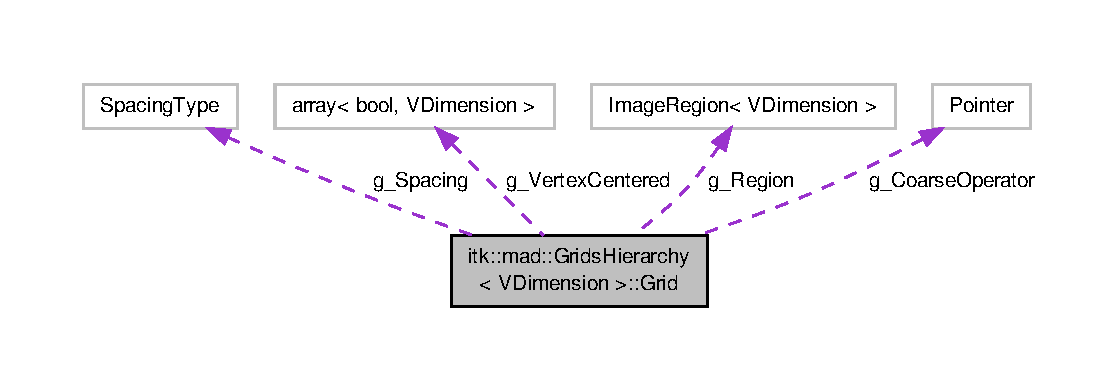
\includegraphics[width=350pt]{structitk_1_1mad_1_1_grids_hierarchy_1_1_grid__coll__graph}
\end{center}
\end{figure}
\subsection*{Public Attributes}
\begin{DoxyCompactItemize}
\item 
\hypertarget{structitk_1_1mad_1_1_grids_hierarchy_1_1_grid_a2381941c2ecb243fe329fb9facb7d28d}{Image\-Region\-Type {\bfseries g\-\_\-\-Region}}\label{structitk_1_1mad_1_1_grids_hierarchy_1_1_grid_a2381941c2ecb243fe329fb9facb7d28d}

\item 
\hypertarget{structitk_1_1mad_1_1_grids_hierarchy_1_1_grid_a6357cf20cdb83ffeb73a8bc921be142f}{Spacing\-Type {\bfseries g\-\_\-\-Spacing}}\label{structitk_1_1mad_1_1_grids_hierarchy_1_1_grid_a6357cf20cdb83ffeb73a8bc921be142f}

\item 
\hypertarget{structitk_1_1mad_1_1_grids_hierarchy_1_1_grid_a35fe66e43347ef491ac7a41e64841bcb}{Stencil\-Image\-Type\-::\-Pointer {\bfseries g\-\_\-\-Coarse\-Operator}}\label{structitk_1_1mad_1_1_grids_hierarchy_1_1_grid_a35fe66e43347ef491ac7a41e64841bcb}

\item 
\hypertarget{structitk_1_1mad_1_1_grids_hierarchy_1_1_grid_ae0d5743811e1b5a941522f3b364b2c3a}{std\-::array$<$ bool, V\-Dimension $>$ {\bfseries g\-\_\-\-Vertex\-Centered}}\label{structitk_1_1mad_1_1_grids_hierarchy_1_1_grid_ae0d5743811e1b5a941522f3b364b2c3a}

\end{DoxyCompactItemize}


\subsection{Detailed Description}
\subsubsection*{template$<$unsigned int V\-Dimension$>$struct itk\-::mad\-::\-Grids\-Hierarchy$<$ V\-Dimension $>$\-::\-Grid}

Raw data structure for each level 

Definition at line 69 of file itk\-Grids\-Hierarchy.\-h.



The documentation for this struct was generated from the following file\-:\begin{DoxyCompactItemize}
\item 
mad/itk\-Grids\-Hierarchy.\-h\end{DoxyCompactItemize}

\hypertarget{classitk_1_1mad_1_1_grids_hierarchy}{\section{itk\-:\-:mad\-:\-:Grids\-Hierarchy$<$ V\-Dimension $>$ Class Template Reference}
\label{classitk_1_1mad_1_1_grids_hierarchy}\index{itk\-::mad\-::\-Grids\-Hierarchy$<$ V\-Dimension $>$@{itk\-::mad\-::\-Grids\-Hierarchy$<$ V\-Dimension $>$}}
}


Class which creates and holds a hierarchy of grids to be used by itk\-Multigrid\-Anisotropic\-Diffusion. It contains informations about each level's grid\-: spacing, region, coarse operator in the form of a pointer to a \hyperlink{classitk_1_1mad_1_1_stencil_image}{Stencil\-Image}, and whether the level was obtained with a vertex centered or a cell centered coarsening (as a convention, level 0 has a vertex centered approach in each direction).  




{\ttfamily \#include $<$itk\-Grids\-Hierarchy.\-h$>$}

\subsection*{Classes}
\begin{DoxyCompactItemize}
\item 
struct \hyperlink{structitk_1_1mad_1_1_grids_hierarchy_1_1_grid}{Grid}
\end{DoxyCompactItemize}
\subsection*{Public Types}
\begin{DoxyCompactItemize}
\item 
typedef double \hyperlink{classitk_1_1mad_1_1_grids_hierarchy_a235005f48422caf216820d2d6b77ca0a}{Precision}
\item 
\hypertarget{classitk_1_1mad_1_1_grids_hierarchy_a4ab641bfee5c8ea9389f304ccd23549f}{typedef \hyperlink{classitk_1_1mad_1_1_grids_hierarchy}{Grids\-Hierarchy} {\bfseries Self}}\label{classitk_1_1mad_1_1_grids_hierarchy_a4ab641bfee5c8ea9389f304ccd23549f}

\item 
\hypertarget{classitk_1_1mad_1_1_grids_hierarchy_a2fee3ed525b2cdf4242351e30f6cce52}{typedef \hyperlink{class_image}{Image}$<$ \hyperlink{classitk_1_1mad_1_1_grids_hierarchy_a235005f48422caf216820d2d6b77ca0a}{Precision}, \\*
V\-Dimension $>$ {\bfseries Image\-Type}}\label{classitk_1_1mad_1_1_grids_hierarchy_a2fee3ed525b2cdf4242351e30f6cce52}

\item 
\hypertarget{classitk_1_1mad_1_1_grids_hierarchy_ac4d01a308c9990adba91abca78a02801}{typedef Neighborhood\\*
$<$ \hyperlink{classitk_1_1mad_1_1_grids_hierarchy_a235005f48422caf216820d2d6b77ca0a}{Precision}, V\-Dimension $>$ {\bfseries Stencil\-Type}}\label{classitk_1_1mad_1_1_grids_hierarchy_ac4d01a308c9990adba91abca78a02801}

\item 
\hypertarget{classitk_1_1mad_1_1_grids_hierarchy_a2417f54fc9001fb7e239e2472c2249a9}{typedef \hyperlink{classitk_1_1mad_1_1_stencil_image}{Stencil\-Image}\\*
$<$ \hyperlink{classitk_1_1mad_1_1_grids_hierarchy_a235005f48422caf216820d2d6b77ca0a}{Precision}, V\-Dimension $>$ {\bfseries Stencil\-Image\-Type}}\label{classitk_1_1mad_1_1_grids_hierarchy_a2417f54fc9001fb7e239e2472c2249a9}

\item 
\hypertarget{classitk_1_1mad_1_1_grids_hierarchy_ab7ed42a7ff14b5a2664efdc50a7505b4}{typedef Image\-Region$<$ V\-Dimension $>$ {\bfseries Image\-Region\-Type}}\label{classitk_1_1mad_1_1_grids_hierarchy_ab7ed42a7ff14b5a2664efdc50a7505b4}

\item 
\hypertarget{classitk_1_1mad_1_1_grids_hierarchy_a48978a328db24d5c9aa98c1fe5faca1f}{typedef Image\-Type\-::\-Spacing\-Type {\bfseries Spacing\-Type}}\label{classitk_1_1mad_1_1_grids_hierarchy_a48978a328db24d5c9aa98c1fe5faca1f}

\item 
\hypertarget{classitk_1_1mad_1_1_grids_hierarchy_a8ae9e2ae3fd0eb0bf300af1e2a158df9}{typedef Image\-Type\-::\-Size\-Type {\bfseries Size\-Type}}\label{classitk_1_1mad_1_1_grids_hierarchy_a8ae9e2ae3fd0eb0bf300af1e2a158df9}

\item 
\hypertarget{classitk_1_1mad_1_1_grids_hierarchy_a5fc892f212cd811c07302ffa89cfb93c}{typedef Image\-Type\-::\-Index\-Type {\bfseries Index\-Type}}\label{classitk_1_1mad_1_1_grids_hierarchy_a5fc892f212cd811c07302ffa89cfb93c}

\end{DoxyCompactItemize}
\subsection*{Public Member Functions}
\begin{DoxyCompactItemize}
\item 
Stencil\-Image\-Type\-::\-Pointer \hyperlink{classitk_1_1mad_1_1_grids_hierarchy_a1fabd3c99e3e7fd81f05f5ceddc35810}{Get\-Coarse\-Operator\-At\-Level} (const unsigned int l) const 
\item 
\hyperlink{structitk_1_1mad_1_1_grids_hierarchy_1_1_grid}{Grid} $\ast$ \hyperlink{classitk_1_1mad_1_1_grids_hierarchy_adbe73da5d41fd62a6aa05405e739633b}{Get\-Grid\-At\-Level} (const unsigned int l)
\item 
Image\-Type\-::\-Pointer \hyperlink{classitk_1_1mad_1_1_grids_hierarchy_a371729b077c35e3367f6ef3e4efc4865}{Create\-Image\-At\-Level} (const unsigned int l) const 
\item 
unsigned int \hyperlink{classitk_1_1mad_1_1_grids_hierarchy_aa1d52d9a52dfd38235f8c78890d457b0}{Get\-Max\-Depth} () const 
\item 
Image\-Region\-Type \hyperlink{classitk_1_1mad_1_1_grids_hierarchy_ab993ed3190b19b4554eb718240258dae}{Get\-Region\-At\-Level} (const unsigned int l) const 
\item 
Spacing\-Type \hyperlink{classitk_1_1mad_1_1_grids_hierarchy_a2c594f9e3a4888666cafa652443e6b2a}{Get\-Spacing\-At\-Level} (const unsigned int l) const 
\item 
std\-::array$<$ bool, V\-Dimension $>$ \hyperlink{classitk_1_1mad_1_1_grids_hierarchy_ac85c588f321ed335bcb282b13afbf05e}{Get\-Vertex\-Centering\-At\-Level} (const unsigned int l) const 
\item 
\hyperlink{classitk_1_1mad_1_1_grids_hierarchy_a7189f95878b8489a473b004d86252467}{Grids\-Hierarchy} (const Image\-Region\-Type \&initial\-Region, const Spacing\-Type \&initial\-Spacing)
\item 
\hyperlink{classitk_1_1mad_1_1_grids_hierarchy_a334910fb2af63d58e2c77774473c55d6}{$\sim$\-Grids\-Hierarchy} ()
\end{DoxyCompactItemize}


\subsection{Detailed Description}
\subsubsection*{template$<$unsigned int V\-Dimension$>$class itk\-::mad\-::\-Grids\-Hierarchy$<$ V\-Dimension $>$}

Class which creates and holds a hierarchy of grids to be used by itk\-Multigrid\-Anisotropic\-Diffusion. It contains informations about each level's grid\-: spacing, region, coarse operator in the form of a pointer to a \hyperlink{classitk_1_1mad_1_1_stencil_image}{Stencil\-Image}, and whether the level was obtained with a vertex centered or a cell centered coarsening (as a convention, level 0 has a vertex centered approach in each direction). 

\begin{DoxyAuthor}{Author}
Antonello Gerbi 
\end{DoxyAuthor}


Definition at line 51 of file itk\-Grids\-Hierarchy.\-h.



\subsection{Member Typedef Documentation}
\hypertarget{classitk_1_1mad_1_1_grids_hierarchy_a235005f48422caf216820d2d6b77ca0a}{\index{itk\-::mad\-::\-Grids\-Hierarchy@{itk\-::mad\-::\-Grids\-Hierarchy}!Precision@{Precision}}
\index{Precision@{Precision}!itk::mad::GridsHierarchy@{itk\-::mad\-::\-Grids\-Hierarchy}}
\subsubsection[{Precision}]{\setlength{\rightskip}{0pt plus 5cm}template$<$unsigned int V\-Dimension$>$ typedef double {\bf itk\-::mad\-::\-Grids\-Hierarchy}$<$ V\-Dimension $>$\-::{\bf Precision}}}\label{classitk_1_1mad_1_1_grids_hierarchy_a235005f48422caf216820d2d6b77ca0a}
Standard class typedefs. 

Definition at line 56 of file itk\-Grids\-Hierarchy.\-h.



\subsection{Constructor \& Destructor Documentation}
\hypertarget{classitk_1_1mad_1_1_grids_hierarchy_a7189f95878b8489a473b004d86252467}{\index{itk\-::mad\-::\-Grids\-Hierarchy@{itk\-::mad\-::\-Grids\-Hierarchy}!Grids\-Hierarchy@{Grids\-Hierarchy}}
\index{Grids\-Hierarchy@{Grids\-Hierarchy}!itk::mad::GridsHierarchy@{itk\-::mad\-::\-Grids\-Hierarchy}}
\subsubsection[{Grids\-Hierarchy}]{\setlength{\rightskip}{0pt plus 5cm}template$<$unsigned int V\-Dimension$>$ {\bf itk\-::mad\-::\-Grids\-Hierarchy}$<$ V\-Dimension $>$\-::{\bf Grids\-Hierarchy} (
\begin{DoxyParamCaption}
\item[{const Image\-Region\-Type \&}]{initial\-Region, }
\item[{const Spacing\-Type \&}]{initial\-Spacing}
\end{DoxyParamCaption}
)}}\label{classitk_1_1mad_1_1_grids_hierarchy_a7189f95878b8489a473b004d86252467}
Class constructor. It needs the grid region and the spacing at level 0. 

Definition at line 32 of file itk\-Grids\-Hierarchy.\-hxx.

\hypertarget{classitk_1_1mad_1_1_grids_hierarchy_a334910fb2af63d58e2c77774473c55d6}{\index{itk\-::mad\-::\-Grids\-Hierarchy@{itk\-::mad\-::\-Grids\-Hierarchy}!$\sim$\-Grids\-Hierarchy@{$\sim$\-Grids\-Hierarchy}}
\index{$\sim$\-Grids\-Hierarchy@{$\sim$\-Grids\-Hierarchy}!itk::mad::GridsHierarchy@{itk\-::mad\-::\-Grids\-Hierarchy}}
\subsubsection[{$\sim$\-Grids\-Hierarchy}]{\setlength{\rightskip}{0pt plus 5cm}template$<$unsigned int V\-Dimension$>$ {\bf itk\-::mad\-::\-Grids\-Hierarchy}$<$ V\-Dimension $>$\-::$\sim${\bf Grids\-Hierarchy} (
\begin{DoxyParamCaption}
{}
\end{DoxyParamCaption}
)}}\label{classitk_1_1mad_1_1_grids_hierarchy_a334910fb2af63d58e2c77774473c55d6}
Class destructor. 

Definition at line 111 of file itk\-Grids\-Hierarchy.\-hxx.



\subsection{Member Function Documentation}
\hypertarget{classitk_1_1mad_1_1_grids_hierarchy_a371729b077c35e3367f6ef3e4efc4865}{\index{itk\-::mad\-::\-Grids\-Hierarchy@{itk\-::mad\-::\-Grids\-Hierarchy}!Create\-Image\-At\-Level@{Create\-Image\-At\-Level}}
\index{Create\-Image\-At\-Level@{Create\-Image\-At\-Level}!itk::mad::GridsHierarchy@{itk\-::mad\-::\-Grids\-Hierarchy}}
\subsubsection[{Create\-Image\-At\-Level}]{\setlength{\rightskip}{0pt plus 5cm}template$<$unsigned int V\-Dimension$>$ {\bf Grids\-Hierarchy}$<$ V\-Dimension $>$\-::Image\-Type\-::\-Pointer {\bf itk\-::mad\-::\-Grids\-Hierarchy}$<$ V\-Dimension $>$\-::Create\-Image\-At\-Level (
\begin{DoxyParamCaption}
\item[{const unsigned int}]{l}
\end{DoxyParamCaption}
) const}}\label{classitk_1_1mad_1_1_grids_hierarchy_a371729b077c35e3367f6ef3e4efc4865}
Creates an empty (allocated but not initialized) defined on level l, and returns a pointer to it. 

Definition at line 188 of file itk\-Grids\-Hierarchy.\-hxx.

\hypertarget{classitk_1_1mad_1_1_grids_hierarchy_a1fabd3c99e3e7fd81f05f5ceddc35810}{\index{itk\-::mad\-::\-Grids\-Hierarchy@{itk\-::mad\-::\-Grids\-Hierarchy}!Get\-Coarse\-Operator\-At\-Level@{Get\-Coarse\-Operator\-At\-Level}}
\index{Get\-Coarse\-Operator\-At\-Level@{Get\-Coarse\-Operator\-At\-Level}!itk::mad::GridsHierarchy@{itk\-::mad\-::\-Grids\-Hierarchy}}
\subsubsection[{Get\-Coarse\-Operator\-At\-Level}]{\setlength{\rightskip}{0pt plus 5cm}template$<$unsigned int V\-Dimension$>$ {\bf Grids\-Hierarchy}$<$ V\-Dimension $>$\-::Stencil\-Image\-Type\-::\-Pointer {\bf itk\-::mad\-::\-Grids\-Hierarchy}$<$ V\-Dimension $>$\-::Get\-Coarse\-Operator\-At\-Level (
\begin{DoxyParamCaption}
\item[{const unsigned int}]{l}
\end{DoxyParamCaption}
) const}}\label{classitk_1_1mad_1_1_grids_hierarchy_a1fabd3c99e3e7fd81f05f5ceddc35810}
Returns pointer to the coarse operator at level l. 

Definition at line 166 of file itk\-Grids\-Hierarchy.\-hxx.

\hypertarget{classitk_1_1mad_1_1_grids_hierarchy_adbe73da5d41fd62a6aa05405e739633b}{\index{itk\-::mad\-::\-Grids\-Hierarchy@{itk\-::mad\-::\-Grids\-Hierarchy}!Get\-Grid\-At\-Level@{Get\-Grid\-At\-Level}}
\index{Get\-Grid\-At\-Level@{Get\-Grid\-At\-Level}!itk::mad::GridsHierarchy@{itk\-::mad\-::\-Grids\-Hierarchy}}
\subsubsection[{Get\-Grid\-At\-Level}]{\setlength{\rightskip}{0pt plus 5cm}template$<$unsigned int V\-Dimension$>$ {\bf Grids\-Hierarchy}$<$ V\-Dimension $>$\-::{\bf Grid} $\ast$ {\bf itk\-::mad\-::\-Grids\-Hierarchy}$<$ V\-Dimension $>$\-::Get\-Grid\-At\-Level (
\begin{DoxyParamCaption}
\item[{const unsigned int}]{l}
\end{DoxyParamCaption}
)}}\label{classitk_1_1mad_1_1_grids_hierarchy_adbe73da5d41fd62a6aa05405e739633b}
Returns pointer to the grid raw data at level l. 

Definition at line 133 of file itk\-Grids\-Hierarchy.\-hxx.

\hypertarget{classitk_1_1mad_1_1_grids_hierarchy_aa1d52d9a52dfd38235f8c78890d457b0}{\index{itk\-::mad\-::\-Grids\-Hierarchy@{itk\-::mad\-::\-Grids\-Hierarchy}!Get\-Max\-Depth@{Get\-Max\-Depth}}
\index{Get\-Max\-Depth@{Get\-Max\-Depth}!itk::mad::GridsHierarchy@{itk\-::mad\-::\-Grids\-Hierarchy}}
\subsubsection[{Get\-Max\-Depth}]{\setlength{\rightskip}{0pt plus 5cm}template$<$unsigned int V\-Dimension$>$ unsigned int {\bf itk\-::mad\-::\-Grids\-Hierarchy}$<$ V\-Dimension $>$\-::Get\-Max\-Depth (
\begin{DoxyParamCaption}
{}
\end{DoxyParamCaption}
) const}}\label{classitk_1_1mad_1_1_grids_hierarchy_aa1d52d9a52dfd38235f8c78890d457b0}
Returns the maximum depth of the hierarchy. 

Definition at line 122 of file itk\-Grids\-Hierarchy.\-hxx.

\hypertarget{classitk_1_1mad_1_1_grids_hierarchy_ab993ed3190b19b4554eb718240258dae}{\index{itk\-::mad\-::\-Grids\-Hierarchy@{itk\-::mad\-::\-Grids\-Hierarchy}!Get\-Region\-At\-Level@{Get\-Region\-At\-Level}}
\index{Get\-Region\-At\-Level@{Get\-Region\-At\-Level}!itk::mad::GridsHierarchy@{itk\-::mad\-::\-Grids\-Hierarchy}}
\subsubsection[{Get\-Region\-At\-Level}]{\setlength{\rightskip}{0pt plus 5cm}template$<$unsigned int V\-Dimension$>$ {\bf Grids\-Hierarchy}$<$ V\-Dimension $>$\-::Image\-Region\-Type {\bf itk\-::mad\-::\-Grids\-Hierarchy}$<$ V\-Dimension $>$\-::Get\-Region\-At\-Level (
\begin{DoxyParamCaption}
\item[{const unsigned int}]{l}
\end{DoxyParamCaption}
) const}}\label{classitk_1_1mad_1_1_grids_hierarchy_ab993ed3190b19b4554eb718240258dae}
Returns the region at level l. 

Definition at line 144 of file itk\-Grids\-Hierarchy.\-hxx.

\hypertarget{classitk_1_1mad_1_1_grids_hierarchy_a2c594f9e3a4888666cafa652443e6b2a}{\index{itk\-::mad\-::\-Grids\-Hierarchy@{itk\-::mad\-::\-Grids\-Hierarchy}!Get\-Spacing\-At\-Level@{Get\-Spacing\-At\-Level}}
\index{Get\-Spacing\-At\-Level@{Get\-Spacing\-At\-Level}!itk::mad::GridsHierarchy@{itk\-::mad\-::\-Grids\-Hierarchy}}
\subsubsection[{Get\-Spacing\-At\-Level}]{\setlength{\rightskip}{0pt plus 5cm}template$<$unsigned int V\-Dimension$>$ {\bf Grids\-Hierarchy}$<$ V\-Dimension $>$\-::Spacing\-Type {\bf itk\-::mad\-::\-Grids\-Hierarchy}$<$ V\-Dimension $>$\-::Get\-Spacing\-At\-Level (
\begin{DoxyParamCaption}
\item[{const unsigned int}]{l}
\end{DoxyParamCaption}
) const}}\label{classitk_1_1mad_1_1_grids_hierarchy_a2c594f9e3a4888666cafa652443e6b2a}
Returns the spacing at level l. 

Definition at line 155 of file itk\-Grids\-Hierarchy.\-hxx.

\hypertarget{classitk_1_1mad_1_1_grids_hierarchy_ac85c588f321ed335bcb282b13afbf05e}{\index{itk\-::mad\-::\-Grids\-Hierarchy@{itk\-::mad\-::\-Grids\-Hierarchy}!Get\-Vertex\-Centering\-At\-Level@{Get\-Vertex\-Centering\-At\-Level}}
\index{Get\-Vertex\-Centering\-At\-Level@{Get\-Vertex\-Centering\-At\-Level}!itk::mad::GridsHierarchy@{itk\-::mad\-::\-Grids\-Hierarchy}}
\subsubsection[{Get\-Vertex\-Centering\-At\-Level}]{\setlength{\rightskip}{0pt plus 5cm}template$<$unsigned int V\-Dimension$>$ std\-::array$<$ bool, V\-Dimension $>$ {\bf itk\-::mad\-::\-Grids\-Hierarchy}$<$ V\-Dimension $>$\-::Get\-Vertex\-Centering\-At\-Level (
\begin{DoxyParamCaption}
\item[{const unsigned int}]{l}
\end{DoxyParamCaption}
) const}}\label{classitk_1_1mad_1_1_grids_hierarchy_ac85c588f321ed335bcb282b13afbf05e}
Returns pointer to the coarse operator at level l. 

Definition at line 177 of file itk\-Grids\-Hierarchy.\-hxx.



The documentation for this class was generated from the following files\-:\begin{DoxyCompactItemize}
\item 
mad/itk\-Grids\-Hierarchy.\-h\item 
mad/itk\-Grids\-Hierarchy.\-hxx\end{DoxyCompactItemize}

\hypertarget{class_image}{\section{Image Class Reference}
\label{class_image}\index{Image@{Image}}
}


Inheritance diagram for Image\-:
\nopagebreak
\begin{figure}[H]
\begin{center}
\leavevmode
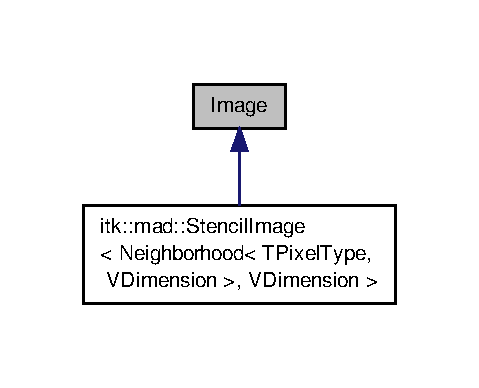
\includegraphics[width=230pt]{class_image__inherit__graph}
\end{center}
\end{figure}


The documentation for this class was generated from the following file\-:\begin{DoxyCompactItemize}
\item 
mad/itk\-Stencil\-Image.\-h\end{DoxyCompactItemize}

\hypertarget{class_image_to_image_filter}{\section{Image\-To\-Image\-Filter Class Reference}
\label{class_image_to_image_filter}\index{Image\-To\-Image\-Filter@{Image\-To\-Image\-Filter}}
}


Inheritance diagram for Image\-To\-Image\-Filter\-:
\nopagebreak
\begin{figure}[H]
\begin{center}
\leavevmode
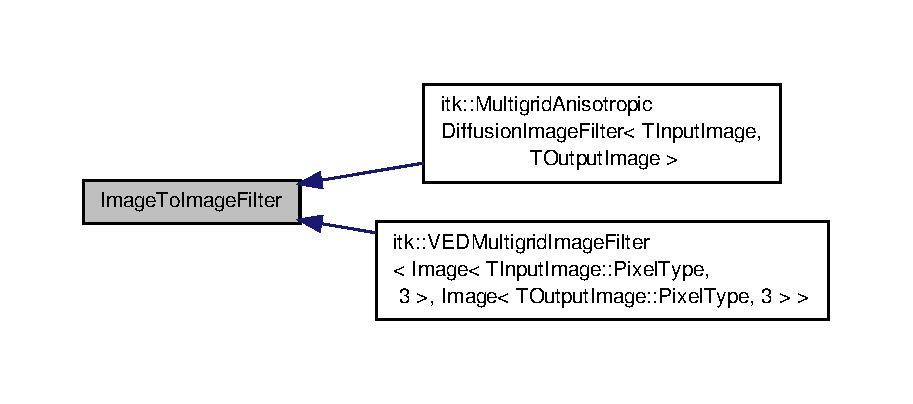
\includegraphics[width=350pt]{class_image_to_image_filter__inherit__graph}
\end{center}
\end{figure}


The documentation for this class was generated from the following file\-:\begin{DoxyCompactItemize}
\item 
itk\-Multigrid\-Anisotropic\-Diffusion\-Image\-Filter.\-h\end{DoxyCompactItemize}

\hypertarget{classitk_1_1mad_1_1_inter_grid_operators}{\section{itk\-:\-:mad\-:\-:Inter\-Grid\-Operators$<$ V\-Dimension $>$ Class Template Reference}
\label{classitk_1_1mad_1_1_inter_grid_operators}\index{itk\-::mad\-::\-Inter\-Grid\-Operators$<$ V\-Dimension $>$@{itk\-::mad\-::\-Inter\-Grid\-Operators$<$ V\-Dimension $>$}}
}


Class implementation of the two inter grid operators. It has to be initialized with an array prescribing which kind of coarsening has to be used between the two grids on each direction\-: vertex centered vs cell centered. It does not need other informations on the grids, as they are extracted from the input image when Interpolation or Restriction are called.  




{\ttfamily \#include $<$itk\-Inter\-Grid\-Operators.\-h$>$}

\subsection*{Public Types}
\begin{DoxyCompactItemize}
\item 
enum \hyperlink{classitk_1_1mad_1_1_inter_grid_operators_a7dfcf280f70ae36e4860d8d962f4a05d}{Point\-Position\-Type} \{ {\bfseries left}, 
{\bfseries interior}, 
{\bfseries right}
 \}
\item 
typedef double \hyperlink{classitk_1_1mad_1_1_inter_grid_operators_ade61ab9b171ac4b689489cb14d3bde7d}{Precision}
\item 
\hypertarget{classitk_1_1mad_1_1_inter_grid_operators_a55328ff18ed00cabde49d578ce4cec2d}{typedef \hyperlink{classitk_1_1mad_1_1_inter_grid_operators}{Inter\-Grid\-Operators} {\bfseries Self}}\label{classitk_1_1mad_1_1_inter_grid_operators_a55328ff18ed00cabde49d578ce4cec2d}

\item 
\hypertarget{classitk_1_1mad_1_1_inter_grid_operators_a6d5bdce33c32c798359046b3baa4658d}{typedef \hyperlink{class_image}{Image}$<$ \hyperlink{classitk_1_1mad_1_1_inter_grid_operators_ade61ab9b171ac4b689489cb14d3bde7d}{Precision}, \\*
V\-Dimension $>$ {\bfseries Image\-Type}}\label{classitk_1_1mad_1_1_inter_grid_operators_a6d5bdce33c32c798359046b3baa4658d}

\item 
\hypertarget{classitk_1_1mad_1_1_inter_grid_operators_ac0d30ff94e6b2d266ebbccb1994e3eb5}{typedef Neighborhood\\*
$<$ \hyperlink{classitk_1_1mad_1_1_inter_grid_operators_ade61ab9b171ac4b689489cb14d3bde7d}{Precision}, V\-Dimension $>$ {\bfseries Stencil\-Type}}\label{classitk_1_1mad_1_1_inter_grid_operators_ac0d30ff94e6b2d266ebbccb1994e3eb5}

\item 
\hypertarget{classitk_1_1mad_1_1_inter_grid_operators_a7221885e733f0b64c02f1975517e8e51}{typedef Image\-Region$<$ V\-Dimension $>$ {\bfseries Image\-Region\-Type}}\label{classitk_1_1mad_1_1_inter_grid_operators_a7221885e733f0b64c02f1975517e8e51}

\item 
\hypertarget{classitk_1_1mad_1_1_inter_grid_operators_a9fce7d83a2d10d6c06db2e36dc6e1eca}{typedef Image\-Type\-::\-Spacing\-Type {\bfseries Spacing\-Type}}\label{classitk_1_1mad_1_1_inter_grid_operators_a9fce7d83a2d10d6c06db2e36dc6e1eca}

\item 
\hypertarget{classitk_1_1mad_1_1_inter_grid_operators_aae9b6fe92d7ff591d1eb14584a52a36e}{typedef Image\-Type\-::\-Size\-Type {\bfseries Size\-Type}}\label{classitk_1_1mad_1_1_inter_grid_operators_aae9b6fe92d7ff591d1eb14584a52a36e}

\item 
\hypertarget{classitk_1_1mad_1_1_inter_grid_operators_ad3726bb2b8dee0d8a53c5fe66a45dbfa}{typedef Image\-Type\-::\-Index\-Type {\bfseries Index\-Type}}\label{classitk_1_1mad_1_1_inter_grid_operators_ad3726bb2b8dee0d8a53c5fe66a45dbfa}

\item 
\hypertarget{classitk_1_1mad_1_1_inter_grid_operators_ad9296508483355dcc2b4cbeb9cf53842}{typedef Image\-Type\-::\-Offset\-Type {\bfseries Offset\-Type}}\label{classitk_1_1mad_1_1_inter_grid_operators_ad9296508483355dcc2b4cbeb9cf53842}

\end{DoxyCompactItemize}
\subsection*{Public Member Functions}
\begin{DoxyCompactItemize}
\item 
\hyperlink{classitk_1_1mad_1_1_inter_grid_operators_ad55220f99bb3317126f3aec19be4c70c}{Inter\-Grid\-Operators} (const std\-::array$<$ bool, V\-Dimension $>$ \&vertex\-Centering)
\item 
\hyperlink{classitk_1_1mad_1_1_inter_grid_operators_a9ae3dcea3ec15339e389163153bc9656}{$\sim$\-Inter\-Grid\-Operators} ()
\item 
Image\-Type\-::\-Pointer \hyperlink{classitk_1_1mad_1_1_inter_grid_operators_a970d50f9b0a8d3815654d36362abfce5}{Interpolation} (const \hyperlink{class_image}{Image\-Type} $\ast$input\-Image, const bool $\ast$ignore\-Left\-Border=nullptr, const bool $\ast$ignore\-Right\-Border=nullptr) const 
\item 
Image\-Type\-::\-Pointer \hyperlink{classitk_1_1mad_1_1_inter_grid_operators_ae99632c351ddaa07d311141c3eb8cd21}{Restriction} (const \hyperlink{class_image}{Image\-Type} $\ast$input\-Image, const bool $\ast$ignore\-Left\-Border=nullptr, const bool $\ast$ignore\-Right\-Border=nullptr) const 
\end{DoxyCompactItemize}


\subsection{Detailed Description}
\subsubsection*{template$<$unsigned int V\-Dimension$>$class itk\-::mad\-::\-Inter\-Grid\-Operators$<$ V\-Dimension $>$}

Class implementation of the two inter grid operators. It has to be initialized with an array prescribing which kind of coarsening has to be used between the two grids on each direction\-: vertex centered vs cell centered. It does not need other informations on the grids, as they are extracted from the input image when Interpolation or Restriction are called. 

\begin{DoxyAuthor}{Author}
Antonello Gerbi 
\end{DoxyAuthor}


Definition at line 48 of file itk\-Inter\-Grid\-Operators.\-h.



\subsection{Member Typedef Documentation}
\hypertarget{classitk_1_1mad_1_1_inter_grid_operators_ade61ab9b171ac4b689489cb14d3bde7d}{\index{itk\-::mad\-::\-Inter\-Grid\-Operators@{itk\-::mad\-::\-Inter\-Grid\-Operators}!Precision@{Precision}}
\index{Precision@{Precision}!itk::mad::InterGridOperators@{itk\-::mad\-::\-Inter\-Grid\-Operators}}
\subsubsection[{Precision}]{\setlength{\rightskip}{0pt plus 5cm}template$<$unsigned int V\-Dimension$>$ typedef double {\bf itk\-::mad\-::\-Inter\-Grid\-Operators}$<$ V\-Dimension $>$\-::{\bf Precision}}}\label{classitk_1_1mad_1_1_inter_grid_operators_ade61ab9b171ac4b689489cb14d3bde7d}
Standard class typedefs. 

Definition at line 53 of file itk\-Inter\-Grid\-Operators.\-h.



\subsection{Member Enumeration Documentation}
\hypertarget{classitk_1_1mad_1_1_inter_grid_operators_a7dfcf280f70ae36e4860d8d962f4a05d}{\index{itk\-::mad\-::\-Inter\-Grid\-Operators@{itk\-::mad\-::\-Inter\-Grid\-Operators}!Point\-Position\-Type@{Point\-Position\-Type}}
\index{Point\-Position\-Type@{Point\-Position\-Type}!itk::mad::InterGridOperators@{itk\-::mad\-::\-Inter\-Grid\-Operators}}
\subsubsection[{Point\-Position\-Type}]{\setlength{\rightskip}{0pt plus 5cm}template$<$unsigned int V\-Dimension$>$ enum {\bf itk\-::mad\-::\-Inter\-Grid\-Operators\-::\-Point\-Position\-Type}}}\label{classitk_1_1mad_1_1_inter_grid_operators_a7dfcf280f70ae36e4860d8d962f4a05d}
Characterization of a point based on its position relative to the interior of the image region. 

Definition at line 66 of file itk\-Inter\-Grid\-Operators.\-h.



\subsection{Constructor \& Destructor Documentation}
\hypertarget{classitk_1_1mad_1_1_inter_grid_operators_ad55220f99bb3317126f3aec19be4c70c}{\index{itk\-::mad\-::\-Inter\-Grid\-Operators@{itk\-::mad\-::\-Inter\-Grid\-Operators}!Inter\-Grid\-Operators@{Inter\-Grid\-Operators}}
\index{Inter\-Grid\-Operators@{Inter\-Grid\-Operators}!itk::mad::InterGridOperators@{itk\-::mad\-::\-Inter\-Grid\-Operators}}
\subsubsection[{Inter\-Grid\-Operators}]{\setlength{\rightskip}{0pt plus 5cm}template$<$unsigned int V\-Dimension$>$ {\bf itk\-::mad\-::\-Inter\-Grid\-Operators}$<$ V\-Dimension $>$\-::{\bf Inter\-Grid\-Operators} (
\begin{DoxyParamCaption}
\item[{const std\-::array$<$ bool, V\-Dimension $>$ \&}]{vertex\-Centering}
\end{DoxyParamCaption}
)}}\label{classitk_1_1mad_1_1_inter_grid_operators_ad55220f99bb3317126f3aec19be4c70c}
Class constructor which takes as argument whether the coarse grid is obtained via vertex centered versus cell centered approach. 

Definition at line 37 of file itk\-Inter\-Grid\-Operators.\-hxx.

\hypertarget{classitk_1_1mad_1_1_inter_grid_operators_a9ae3dcea3ec15339e389163153bc9656}{\index{itk\-::mad\-::\-Inter\-Grid\-Operators@{itk\-::mad\-::\-Inter\-Grid\-Operators}!$\sim$\-Inter\-Grid\-Operators@{$\sim$\-Inter\-Grid\-Operators}}
\index{$\sim$\-Inter\-Grid\-Operators@{$\sim$\-Inter\-Grid\-Operators}!itk::mad::InterGridOperators@{itk\-::mad\-::\-Inter\-Grid\-Operators}}
\subsubsection[{$\sim$\-Inter\-Grid\-Operators}]{\setlength{\rightskip}{0pt plus 5cm}template$<$unsigned int V\-Dimension$>$ {\bf itk\-::mad\-::\-Inter\-Grid\-Operators}$<$ V\-Dimension $>$\-::$\sim${\bf Inter\-Grid\-Operators} (
\begin{DoxyParamCaption}
{}
\end{DoxyParamCaption}
)\hspace{0.3cm}{\ttfamily [inline]}}}\label{classitk_1_1mad_1_1_inter_grid_operators_a9ae3dcea3ec15339e389163153bc9656}
Class destructor. 

Definition at line 73 of file itk\-Inter\-Grid\-Operators.\-h.



\subsection{Member Function Documentation}
\hypertarget{classitk_1_1mad_1_1_inter_grid_operators_a970d50f9b0a8d3815654d36362abfce5}{\index{itk\-::mad\-::\-Inter\-Grid\-Operators@{itk\-::mad\-::\-Inter\-Grid\-Operators}!Interpolation@{Interpolation}}
\index{Interpolation@{Interpolation}!itk::mad::InterGridOperators@{itk\-::mad\-::\-Inter\-Grid\-Operators}}
\subsubsection[{Interpolation}]{\setlength{\rightskip}{0pt plus 5cm}template$<$unsigned int V\-Dimension$>$ {\bf Inter\-Grid\-Operators}$<$ V\-Dimension $>$\-::Image\-Type\-::\-Pointer {\bf itk\-::mad\-::\-Inter\-Grid\-Operators}$<$ V\-Dimension $>$\-::Interpolation (
\begin{DoxyParamCaption}
\item[{const {\bf Image\-Type} $\ast$}]{input\-Image, }
\item[{const bool $\ast$}]{ignore\-Left\-Border = {\ttfamily nullptr}, }
\item[{const bool $\ast$}]{ignore\-Right\-Border = {\ttfamily nullptr}}
\end{DoxyParamCaption}
) const}}\label{classitk_1_1mad_1_1_inter_grid_operators_a970d50f9b0a8d3815654d36362abfce5}
Interpolation operator. It optionally accepts an array whose boolean values prescribe if the border points, on the left and right side of each direction, has to be restricted with the same stencil as that of interior points. 

Definition at line 48 of file itk\-Inter\-Grid\-Operators.\-hxx.

\hypertarget{classitk_1_1mad_1_1_inter_grid_operators_ae99632c351ddaa07d311141c3eb8cd21}{\index{itk\-::mad\-::\-Inter\-Grid\-Operators@{itk\-::mad\-::\-Inter\-Grid\-Operators}!Restriction@{Restriction}}
\index{Restriction@{Restriction}!itk::mad::InterGridOperators@{itk\-::mad\-::\-Inter\-Grid\-Operators}}
\subsubsection[{Restriction}]{\setlength{\rightskip}{0pt plus 5cm}template$<$unsigned int V\-Dimension$>$ {\bf Inter\-Grid\-Operators}$<$ V\-Dimension $>$\-::Image\-Type\-::\-Pointer {\bf itk\-::mad\-::\-Inter\-Grid\-Operators}$<$ V\-Dimension $>$\-::Restriction (
\begin{DoxyParamCaption}
\item[{const {\bf Image\-Type} $\ast$}]{input\-Image, }
\item[{const bool $\ast$}]{ignore\-Left\-Border = {\ttfamily nullptr}, }
\item[{const bool $\ast$}]{ignore\-Right\-Border = {\ttfamily nullptr}}
\end{DoxyParamCaption}
) const}}\label{classitk_1_1mad_1_1_inter_grid_operators_ae99632c351ddaa07d311141c3eb8cd21}
Restriction operator. It optionally accepts an array whose boolean values prescribe if the border points, on the left and right side of each direction, has to be restricted with the same stencil as that of interior points. 

Definition at line 181 of file itk\-Inter\-Grid\-Operators.\-hxx.



The documentation for this class was generated from the following files\-:\begin{DoxyCompactItemize}
\item 
mad/itk\-Inter\-Grid\-Operators.\-h\item 
mad/itk\-Inter\-Grid\-Operators.\-hxx\end{DoxyCompactItemize}

\hypertarget{classitk_1_1_multigrid_anisotropic_diffusion_image_filter}{\section{itk\-:\-:Multigrid\-Anisotropic\-Diffusion\-Image\-Filter$<$ T\-Input\-Image, T\-Output\-Image, T\-Smoother\-Type $>$ Class Template Reference}
\label{classitk_1_1_multigrid_anisotropic_diffusion_image_filter}\index{itk\-::\-Multigrid\-Anisotropic\-Diffusion\-Image\-Filter$<$ T\-Input\-Image, T\-Output\-Image, T\-Smoother\-Type $>$@{itk\-::\-Multigrid\-Anisotropic\-Diffusion\-Image\-Filter$<$ T\-Input\-Image, T\-Output\-Image, T\-Smoother\-Type $>$}}
}


This class embodies, in the form of an \hyperlink{class_image_to_image_filter}{Image\-To\-Image\-Filter} class, an implementation of a multigrid method to solve a generic anisotropic diffusion problem\-:  




{\ttfamily \#include $<$itk\-Multigrid\-Anisotropic\-Diffusion\-Image\-Filter.\-h$>$}



Inheritance diagram for itk\-:\-:Multigrid\-Anisotropic\-Diffusion\-Image\-Filter$<$ T\-Input\-Image, T\-Output\-Image, T\-Smoother\-Type $>$\-:
\nopagebreak
\begin{figure}[H]
\begin{center}
\leavevmode
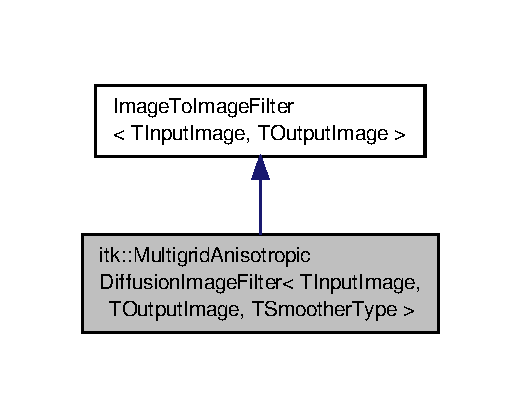
\includegraphics[width=250pt]{classitk_1_1_multigrid_anisotropic_diffusion_image_filter__inherit__graph}
\end{center}
\end{figure}


Collaboration diagram for itk\-:\-:Multigrid\-Anisotropic\-Diffusion\-Image\-Filter$<$ T\-Input\-Image, T\-Output\-Image, T\-Smoother\-Type $>$\-:
\nopagebreak
\begin{figure}[H]
\begin{center}
\leavevmode
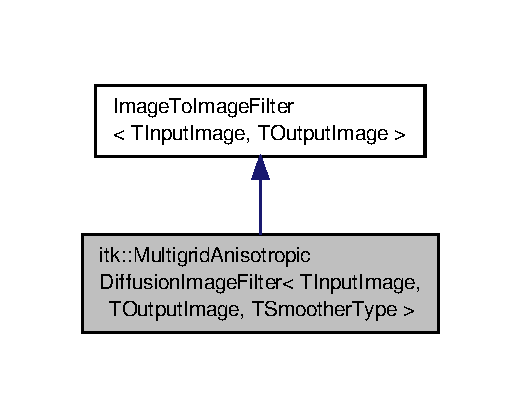
\includegraphics[width=250pt]{classitk_1_1_multigrid_anisotropic_diffusion_image_filter__coll__graph}
\end{center}
\end{figure}
\subsection*{Public Types}
\begin{DoxyCompactItemize}
\item 
enum {\bfseries Cycle\-Type} \{ {\bfseries V\-C\-Y\-C\-L\-E}, 
{\bfseries F\-M\-G}, 
{\bfseries S\-M\-O\-O\-T\-H\-E\-R}
 \}
\item 
typedef \\*
\hyperlink{classitk_1_1_multigrid_anisotropic_diffusion_image_filter}{Multigrid\-Anisotropic\-Diffusion\-Image\-Filter} \hyperlink{classitk_1_1_multigrid_anisotropic_diffusion_image_filter_a7a4e0d1647645c6de01cb808db77bc5a}{Self}
\item 
\hypertarget{classitk_1_1_multigrid_anisotropic_diffusion_image_filter_ab6e9fe3918a768ae1e14d785f2ad8e36}{typedef \hyperlink{class_image_to_image_filter}{Image\-To\-Image\-Filter}\\*
$<$ T\-Input\-Image, T\-Output\-Image $>$ {\bfseries Super\-Class}}\label{classitk_1_1_multigrid_anisotropic_diffusion_image_filter_ab6e9fe3918a768ae1e14d785f2ad8e36}

\item 
\hypertarget{classitk_1_1_multigrid_anisotropic_diffusion_image_filter_ab01db8d5b9b3fd8b955e63b3c38138b6}{typedef Smart\-Pointer$<$ \hyperlink{classitk_1_1_multigrid_anisotropic_diffusion_image_filter_a7a4e0d1647645c6de01cb808db77bc5a}{Self} $>$ {\bfseries Pointer}}\label{classitk_1_1_multigrid_anisotropic_diffusion_image_filter_ab01db8d5b9b3fd8b955e63b3c38138b6}

\item 
\hypertarget{classitk_1_1_multigrid_anisotropic_diffusion_image_filter_a1ba3f17f7f1e7fc199a60e30b30a0946}{typedef Smart\-Pointer$<$ const \hyperlink{classitk_1_1_multigrid_anisotropic_diffusion_image_filter_a7a4e0d1647645c6de01cb808db77bc5a}{Self} $>$ {\bfseries Const\-Pointer}}\label{classitk_1_1_multigrid_anisotropic_diffusion_image_filter_a1ba3f17f7f1e7fc199a60e30b30a0946}

\item 
\hypertarget{classitk_1_1_multigrid_anisotropic_diffusion_image_filter_a3f91cd5dff5b6d570a2b8d5b76484e38}{typedef T\-Input\-Image {\bfseries Input\-Image\-Type}}\label{classitk_1_1_multigrid_anisotropic_diffusion_image_filter_a3f91cd5dff5b6d570a2b8d5b76484e38}

\item 
\hypertarget{classitk_1_1_multigrid_anisotropic_diffusion_image_filter_a94aac911a4076c51758abe6747ed9b65}{typedef T\-Input\-Image\-::\-Pixel\-Type {\bfseries Input\-Pixel\-Type}}\label{classitk_1_1_multigrid_anisotropic_diffusion_image_filter_a94aac911a4076c51758abe6747ed9b65}

\item 
\hypertarget{classitk_1_1_multigrid_anisotropic_diffusion_image_filter_aa81c0f20db5dbf5cf46f3b6e9dc7f569}{typedef T\-Output\-Image {\bfseries Output\-Image\-Type}}\label{classitk_1_1_multigrid_anisotropic_diffusion_image_filter_aa81c0f20db5dbf5cf46f3b6e9dc7f569}

\item 
\hypertarget{classitk_1_1_multigrid_anisotropic_diffusion_image_filter_ad02c604083fd2fce15aa12fa9bf8d7f0}{typedef T\-Output\-Image\-::\-Pixel\-Type {\bfseries Output\-Pixel\-Type}}\label{classitk_1_1_multigrid_anisotropic_diffusion_image_filter_ad02c604083fd2fce15aa12fa9bf8d7f0}

\item 
\hypertarget{classitk_1_1_multigrid_anisotropic_diffusion_image_filter_a9df6a18ac8f39a8a038929943dc90895}{typedef double {\bfseries Internal\-Pixel\-Type}}\label{classitk_1_1_multigrid_anisotropic_diffusion_image_filter_a9df6a18ac8f39a8a038929943dc90895}

\item 
\hypertarget{classitk_1_1_multigrid_anisotropic_diffusion_image_filter_a295ecd99b5dbcde22c6b1188852c074a}{typedef \hyperlink{class_image}{Image}\\*
$<$ Internal\-Pixel\-Type, \\*
T\-Input\-Image\-::\-Image\-Dimension $>$ {\bfseries Internal\-Image\-Type}}\label{classitk_1_1_multigrid_anisotropic_diffusion_image_filter_a295ecd99b5dbcde22c6b1188852c074a}

\item 
\hypertarget{classitk_1_1_multigrid_anisotropic_diffusion_image_filter_aa903243f030c7ccb09f28425cc5078e5}{typedef \hyperlink{class_image}{Image}\\*
$<$ Symmetric\-Second\-Rank\-Tensor\\*
$<$ Input\-Pixel\-Type, \\*
T\-Input\-Image\-::\-Image\-Dimension $>$\\*
, T\-Input\-Image\-::\-Image\-Dimension $>$ {\bfseries Input\-Tensor\-Image\-Type}}\label{classitk_1_1_multigrid_anisotropic_diffusion_image_filter_aa903243f030c7ccb09f28425cc5078e5}

\item 
\hypertarget{classitk_1_1_multigrid_anisotropic_diffusion_image_filter_aa2deb984a182d33b1079d727fc41dc04}{typedef \hyperlink{class_image}{Image}\\*
$<$ Symmetric\-Second\-Rank\-Tensor\\*
$<$ Internal\-Pixel\-Type, \\*
T\-Input\-Image\-::\-Image\-Dimension $>$\\*
, T\-Input\-Image\-::\-Image\-Dimension $>$ {\bfseries Internal\-Tensor\-Image\-Type}}\label{classitk_1_1_multigrid_anisotropic_diffusion_image_filter_aa2deb984a182d33b1079d727fc41dc04}

\item 
\hypertarget{classitk_1_1_multigrid_anisotropic_diffusion_image_filter_a6bb63b70b7d5b408fe4c6adee053bf73}{typedef \hyperlink{classitk_1_1mad_1_1_stencil_image}{mad\-::\-Stencil\-Image}\\*
$<$ Internal\-Pixel\-Type, \\*
T\-Input\-Image\-::\-Image\-Dimension $>$ {\bfseries Stencil\-Image\-Type}}\label{classitk_1_1_multigrid_anisotropic_diffusion_image_filter_a6bb63b70b7d5b408fe4c6adee053bf73}

\item 
\hypertarget{classitk_1_1_multigrid_anisotropic_diffusion_image_filter_a32c49de5ba3cae3731c4b973839a49a4}{typedef \hyperlink{classitk_1_1mad_1_1_grids_hierarchy}{mad\-::\-Grids\-Hierarchy}\\*
$<$ T\-Input\-Image\-::\-Image\-Dimension $>$ {\bfseries Grids\-Hierarchy\-Type}}\label{classitk_1_1_multigrid_anisotropic_diffusion_image_filter_a32c49de5ba3cae3731c4b973839a49a4}

\item 
\hypertarget{classitk_1_1_multigrid_anisotropic_diffusion_image_filter_ac2321112a8bd8744172c4762afecab3c}{typedef \\*
\hyperlink{classitk_1_1mad_1_1_inter_grid_operators}{mad\-::\-Inter\-Grid\-Operators}\\*
$<$ T\-Input\-Image\-::\-Image\-Dimension $>$ {\bfseries Inter\-Grid\-Operators\-Type}}\label{classitk_1_1_multigrid_anisotropic_diffusion_image_filter_ac2321112a8bd8744172c4762afecab3c}

\item 
\hypertarget{classitk_1_1_multigrid_anisotropic_diffusion_image_filter_a92e843466625b157020146038918e46c}{typedef \\*
\hyperlink{classitk_1_1mad_1_1_coarse_grid_operators_generator}{mad\-::\-Coarse\-Grid\-Operators\-Generator}\\*
$<$ T\-Input\-Image\-::\-Image\-Dimension $>$ {\bfseries Coarse\-Grid\-Operators\-Generator\-Type}}\label{classitk_1_1_multigrid_anisotropic_diffusion_image_filter_a92e843466625b157020146038918e46c}

\item 
\hypertarget{classitk_1_1_multigrid_anisotropic_diffusion_image_filter_a215b1578facc40704aa17ea36ee2eafa}{typedef \\*
\hyperlink{classitk_1_1mad_1_1_coarse_grid_operators_generator}{mad\-::\-Coarse\-Grid\-Operators\-Generator}\\*
$<$ T\-Input\-Image\-::\-Image\-Dimension $>$\\*
\-::Coarse\-Grid\-Operator\-Type {\bfseries Coarse\-Grid\-Operator\-Type}}\label{classitk_1_1_multigrid_anisotropic_diffusion_image_filter_a215b1578facc40704aa17ea36ee2eafa}

\item 
\hypertarget{classitk_1_1_multigrid_anisotropic_diffusion_image_filter_ab81d2b899931e2542b5be0d46bd5ca9d}{typedef \hyperlink{classitk_1_1mad_1_1_direct_solver}{mad\-::\-Direct\-Solver}\\*
$<$ T\-Input\-Image\-::\-Image\-Dimension $>$ {\bfseries Direct\-Solver\-Type}}\label{classitk_1_1_multigrid_anisotropic_diffusion_image_filter_ab81d2b899931e2542b5be0d46bd5ca9d}

\item 
\hypertarget{classitk_1_1_multigrid_anisotropic_diffusion_image_filter_a871cc815201beb54f12674523041c9e1}{typedef Internal\-Pixel\-Type {\bfseries Precision}}\label{classitk_1_1_multigrid_anisotropic_diffusion_image_filter_a871cc815201beb54f12674523041c9e1}

\end{DoxyCompactItemize}
\subsection*{Public Member Functions}
\begin{DoxyCompactItemize}
\item 
\hyperlink{classitk_1_1_multigrid_anisotropic_diffusion_image_filter_a6e4ed4edbd2bc2eaabe60a3f7a82e285}{itk\-New\-Macro} (\hyperlink{classitk_1_1_multigrid_anisotropic_diffusion_image_filter_a7a4e0d1647645c6de01cb808db77bc5a}{Self})
\item 
\hyperlink{classitk_1_1_multigrid_anisotropic_diffusion_image_filter_a08dfe44efe545d6203dcab33c6e7d31e}{itk\-Type\-Macro} (\hyperlink{classitk_1_1_multigrid_anisotropic_diffusion_image_filter}{Multigrid\-Anisotropic\-Diffusion\-Image\-Filter}, \hyperlink{class_image_to_image_filter}{Image\-To\-Image\-Filter})
\item 
\hyperlink{classitk_1_1_multigrid_anisotropic_diffusion_image_filter_a470139536f9b713f6190692ddd6ae2bb}{itk\-Set\-Macro} (Coarse\-Grid\-Operator, Coarse\-Grid\-Operator\-Type)
\item 
\hyperlink{classitk_1_1_multigrid_anisotropic_diffusion_image_filter_a9154f4d2eec6366a5c0c64ee6dba2a42}{itk\-Set\-Macro} (Cycle, Cycle\-Type)
\item 
\hyperlink{classitk_1_1_multigrid_anisotropic_diffusion_image_filter_a30335e558311f46eba513a80ea27505c}{itk\-Set\-Macro} (Iterations\-Per\-Grid, unsigned int)
\item 
\hyperlink{classitk_1_1_multigrid_anisotropic_diffusion_image_filter_a579f69c9706b4f844df0c85fcf6d3ddb}{itk\-Set\-Macro} (Max\-Cycles, unsigned int)
\item 
\hyperlink{classitk_1_1_multigrid_anisotropic_diffusion_image_filter_a5fd91b79f46859bdf2640043854fd011}{itk\-Set\-Macro} (Number\-Of\-Steps, unsigned int)
\item 
\hyperlink{classitk_1_1_multigrid_anisotropic_diffusion_image_filter_aee6ab94268911e771f826467095af499}{itk\-Set\-Macro} (Time\-Step, Precision)
\item 
\hyperlink{classitk_1_1_multigrid_anisotropic_diffusion_image_filter_a4f5dcab9135cae277d1bfb14272fbe69}{itk\-Set\-Macro} (Tolerance, Precision)
\item 
\hyperlink{classitk_1_1_multigrid_anisotropic_diffusion_image_filter_a06efb7a8c22f1f35a6709f6731416a30}{itk\-Set\-Macro} (Verbose, bool)
\item 
void \hyperlink{classitk_1_1_multigrid_anisotropic_diffusion_image_filter_a8138ea70b96f470cdffc5b488d334b0f}{Set\-Diffusion\-Tensor} (const \hyperlink{class_image}{Input\-Tensor\-Image\-Type} $\ast$input\-Tensor)
\item 
void \hyperlink{classitk_1_1_multigrid_anisotropic_diffusion_image_filter_ac823dce9a05730f0f1f871c4d7799bcf}{Set\-Input} (const Input\-Image\-Type $\ast$input\-Image)
\end{DoxyCompactItemize}
\subsection*{Protected Member Functions}
\begin{DoxyCompactItemize}
\item 
\hyperlink{classitk_1_1_multigrid_anisotropic_diffusion_image_filter_a18f400ab67bf4ea3b351dcf0e0fd5875}{Multigrid\-Anisotropic\-Diffusion\-Image\-Filter} ()
\item 
\hyperlink{classitk_1_1_multigrid_anisotropic_diffusion_image_filter_aa77a44fd7e8871eaa154d2c1b12d2781}{$\sim$\-Multigrid\-Anisotropic\-Diffusion\-Image\-Filter} ()
\item 
virtual void \hyperlink{classitk_1_1_multigrid_anisotropic_diffusion_image_filter_a7229e9367c9f99c4838bd75b71bdce9b}{Generate\-Data} ()
\end{DoxyCompactItemize}


\subsection{Detailed Description}
\subsubsection*{template$<$class T\-Input\-Image, class T\-Output\-Image, class T\-Smoother\-Type = mad\-::\-Multigrid\-Gauss\-Seidel\-Smoother$<$ T\-Input\-Image\-::\-Image\-Dimension $>$$>$class itk\-::\-Multigrid\-Anisotropic\-Diffusion\-Image\-Filter$<$ T\-Input\-Image, T\-Output\-Image, T\-Smoother\-Type $>$}

This class embodies, in the form of an \hyperlink{class_image_to_image_filter}{Image\-To\-Image\-Filter} class, an implementation of a multigrid method to solve a generic anisotropic diffusion problem\-: 

\[ \partial_t I(\mathbf{x}, t) - \mathrm{div} \left( M(\mathbf{x}) \nabla I(\mathbf{x}, t) \right) = 0 \]

The filter is templated, in addition to the input and output image types, over the smoother type; the latter should be a derived class of the pure virtual base class Multigrid\-Smoother. The smoothers Multigrid\-Gauss\-Seidel (which is the default one if not specified) and Multigrid\-Weighted\-Jacobi have already been implemented, and can be found in the subdirectory .mad/ .

The minimum inputs required for the filter to work are\-:


\begin{DoxyEnumerate}
\item The image to be diffused
\item A diffusion tensor in the form of an image with a Symmetric\-Second\-Rank\-Tensor as pixel type
\end{DoxyEnumerate}

The image and the tensor must be defined on the same Image\-Region. Optional parameters are\-:


\begin{DoxyEnumerate}
\item The time step (defaults to 0.\-01)
\item The number of time steps (defaults to 1)
\item The type of coarse grid operator to build, the options being Direct Coarse Approximation (D\-C\-A) and Galerkin Coarse Approximation (G\-C\-A) (defaults to D\-C\-A)
\item The type of cycle to be executed\-: F\-M\-G, V\-C\-Y\-C\-L\-E and S\-M\-O\-O\-T\-H\-E\-R (in the last two cases, the initial guess is the image at the previous step). F\-M\-G and V\-C\-Y\-C\-L\-E are well-\/known multigrid cycles. The S\-M\-O\-O\-T\-H\-E\-R mode solves the problem using the chosen smoother only, and is mainly intended as a baseline for comparison with the first two. (defaults to V\-C\-Y\-C\-L\-E).
\item The number of smoother iterations for each level (defaults to 2)
\item The maximum relative residual tolerance (defaults to 1e-\/6)
\item The maximum number of V\-Cycles (defaults to 100)
\item The verbosity (defaults to 0 = quiet)
\end{DoxyEnumerate}

The filter works with double type as internal precision. The coefficients of the Symmetric\-Second\-Rank\-Tensor elements composing the diffusion tensor are expected to have the same type as the input image.

\begin{DoxyAuthor}{Author}
Antonello Gerbi 
\end{DoxyAuthor}


Definition at line 91 of file itk\-Multigrid\-Anisotropic\-Diffusion\-Image\-Filter.\-h.



\subsection{Member Typedef Documentation}
\hypertarget{classitk_1_1_multigrid_anisotropic_diffusion_image_filter_a7a4e0d1647645c6de01cb808db77bc5a}{\index{itk\-::\-Multigrid\-Anisotropic\-Diffusion\-Image\-Filter@{itk\-::\-Multigrid\-Anisotropic\-Diffusion\-Image\-Filter}!Self@{Self}}
\index{Self@{Self}!itk::MultigridAnisotropicDiffusionImageFilter@{itk\-::\-Multigrid\-Anisotropic\-Diffusion\-Image\-Filter}}
\subsubsection[{Self}]{\setlength{\rightskip}{0pt plus 5cm}template$<$class T\-Input\-Image, class T\-Output\-Image, class T\-Smoother\-Type = mad\-::\-Multigrid\-Gauss\-Seidel\-Smoother$<$ T\-Input\-Image\-::\-Image\-Dimension $>$$>$ typedef {\bf Multigrid\-Anisotropic\-Diffusion\-Image\-Filter} {\bf itk\-::\-Multigrid\-Anisotropic\-Diffusion\-Image\-Filter}$<$ T\-Input\-Image, T\-Output\-Image, T\-Smoother\-Type $>$\-::{\bf Self}}}\label{classitk_1_1_multigrid_anisotropic_diffusion_image_filter_a7a4e0d1647645c6de01cb808db77bc5a}
Standard and useful class typedefs. 

Definition at line 97 of file itk\-Multigrid\-Anisotropic\-Diffusion\-Image\-Filter.\-h.



\subsection{Constructor \& Destructor Documentation}
\hypertarget{classitk_1_1_multigrid_anisotropic_diffusion_image_filter_a18f400ab67bf4ea3b351dcf0e0fd5875}{\index{itk\-::\-Multigrid\-Anisotropic\-Diffusion\-Image\-Filter@{itk\-::\-Multigrid\-Anisotropic\-Diffusion\-Image\-Filter}!Multigrid\-Anisotropic\-Diffusion\-Image\-Filter@{Multigrid\-Anisotropic\-Diffusion\-Image\-Filter}}
\index{Multigrid\-Anisotropic\-Diffusion\-Image\-Filter@{Multigrid\-Anisotropic\-Diffusion\-Image\-Filter}!itk::MultigridAnisotropicDiffusionImageFilter@{itk\-::\-Multigrid\-Anisotropic\-Diffusion\-Image\-Filter}}
\subsubsection[{Multigrid\-Anisotropic\-Diffusion\-Image\-Filter}]{\setlength{\rightskip}{0pt plus 5cm}template$<$class T\-Input\-Image , class T\-Output\-Image , class T\-Smoother\-Type $>$ {\bf itk\-::\-Multigrid\-Anisotropic\-Diffusion\-Image\-Filter}$<$ T\-Input\-Image, T\-Output\-Image, T\-Smoother\-Type $>$\-::{\bf Multigrid\-Anisotropic\-Diffusion\-Image\-Filter} (
\begin{DoxyParamCaption}
{}
\end{DoxyParamCaption}
)\hspace{0.3cm}{\ttfamily [protected]}}}\label{classitk_1_1_multigrid_anisotropic_diffusion_image_filter_a18f400ab67bf4ea3b351dcf0e0fd5875}
Class constructor. 

Definition at line 38 of file itk\-Multigrid\-Anisotropic\-Diffusion\-Image\-Filter.\-hxx.

\hypertarget{classitk_1_1_multigrid_anisotropic_diffusion_image_filter_aa77a44fd7e8871eaa154d2c1b12d2781}{\index{itk\-::\-Multigrid\-Anisotropic\-Diffusion\-Image\-Filter@{itk\-::\-Multigrid\-Anisotropic\-Diffusion\-Image\-Filter}!$\sim$\-Multigrid\-Anisotropic\-Diffusion\-Image\-Filter@{$\sim$\-Multigrid\-Anisotropic\-Diffusion\-Image\-Filter}}
\index{$\sim$\-Multigrid\-Anisotropic\-Diffusion\-Image\-Filter@{$\sim$\-Multigrid\-Anisotropic\-Diffusion\-Image\-Filter}!itk::MultigridAnisotropicDiffusionImageFilter@{itk\-::\-Multigrid\-Anisotropic\-Diffusion\-Image\-Filter}}
\subsubsection[{$\sim$\-Multigrid\-Anisotropic\-Diffusion\-Image\-Filter}]{\setlength{\rightskip}{0pt plus 5cm}template$<$class T\-Input\-Image , class T\-Output\-Image , class T\-Smoother\-Type $>$ {\bf itk\-::\-Multigrid\-Anisotropic\-Diffusion\-Image\-Filter}$<$ T\-Input\-Image, T\-Output\-Image, T\-Smoother\-Type $>$\-::$\sim${\bf Multigrid\-Anisotropic\-Diffusion\-Image\-Filter} (
\begin{DoxyParamCaption}
{}
\end{DoxyParamCaption}
)\hspace{0.3cm}{\ttfamily [protected]}}}\label{classitk_1_1_multigrid_anisotropic_diffusion_image_filter_aa77a44fd7e8871eaa154d2c1b12d2781}
Class destructor. 

Definition at line 58 of file itk\-Multigrid\-Anisotropic\-Diffusion\-Image\-Filter.\-hxx.



\subsection{Member Function Documentation}
\hypertarget{classitk_1_1_multigrid_anisotropic_diffusion_image_filter_a7229e9367c9f99c4838bd75b71bdce9b}{\index{itk\-::\-Multigrid\-Anisotropic\-Diffusion\-Image\-Filter@{itk\-::\-Multigrid\-Anisotropic\-Diffusion\-Image\-Filter}!Generate\-Data@{Generate\-Data}}
\index{Generate\-Data@{Generate\-Data}!itk::MultigridAnisotropicDiffusionImageFilter@{itk\-::\-Multigrid\-Anisotropic\-Diffusion\-Image\-Filter}}
\subsubsection[{Generate\-Data}]{\setlength{\rightskip}{0pt plus 5cm}template$<$class T\-Input\-Image , class T\-Output\-Image , class T\-Smoother\-Type $>$ void {\bf itk\-::\-Multigrid\-Anisotropic\-Diffusion\-Image\-Filter}$<$ T\-Input\-Image, T\-Output\-Image, T\-Smoother\-Type $>$\-::Generate\-Data (
\begin{DoxyParamCaption}
{}
\end{DoxyParamCaption}
)\hspace{0.3cm}{\ttfamily [protected]}, {\ttfamily [virtual]}}}\label{classitk_1_1_multigrid_anisotropic_diffusion_image_filter_a7229e9367c9f99c4838bd75b71bdce9b}
Generates the output, which is then accessed by method Get\-Ouput(). 

Definition at line 119 of file itk\-Multigrid\-Anisotropic\-Diffusion\-Image\-Filter.\-hxx.

\hypertarget{classitk_1_1_multigrid_anisotropic_diffusion_image_filter_a6e4ed4edbd2bc2eaabe60a3f7a82e285}{\index{itk\-::\-Multigrid\-Anisotropic\-Diffusion\-Image\-Filter@{itk\-::\-Multigrid\-Anisotropic\-Diffusion\-Image\-Filter}!itk\-New\-Macro@{itk\-New\-Macro}}
\index{itk\-New\-Macro@{itk\-New\-Macro}!itk::MultigridAnisotropicDiffusionImageFilter@{itk\-::\-Multigrid\-Anisotropic\-Diffusion\-Image\-Filter}}
\subsubsection[{itk\-New\-Macro}]{\setlength{\rightskip}{0pt plus 5cm}template$<$class T\-Input\-Image, class T\-Output\-Image, class T\-Smoother\-Type = mad\-::\-Multigrid\-Gauss\-Seidel\-Smoother$<$ T\-Input\-Image\-::\-Image\-Dimension $>$$>$ {\bf itk\-::\-Multigrid\-Anisotropic\-Diffusion\-Image\-Filter}$<$ T\-Input\-Image, T\-Output\-Image, T\-Smoother\-Type $>$\-::itk\-New\-Macro (
\begin{DoxyParamCaption}
\item[{{\bf Self}}]{}
\end{DoxyParamCaption}
)}}\label{classitk_1_1_multigrid_anisotropic_diffusion_image_filter_a6e4ed4edbd2bc2eaabe60a3f7a82e285}
Method for creation through the object factory. \hypertarget{classitk_1_1_multigrid_anisotropic_diffusion_image_filter_a470139536f9b713f6190692ddd6ae2bb}{\index{itk\-::\-Multigrid\-Anisotropic\-Diffusion\-Image\-Filter@{itk\-::\-Multigrid\-Anisotropic\-Diffusion\-Image\-Filter}!itk\-Set\-Macro@{itk\-Set\-Macro}}
\index{itk\-Set\-Macro@{itk\-Set\-Macro}!itk::MultigridAnisotropicDiffusionImageFilter@{itk\-::\-Multigrid\-Anisotropic\-Diffusion\-Image\-Filter}}
\subsubsection[{itk\-Set\-Macro}]{\setlength{\rightskip}{0pt plus 5cm}template$<$class T\-Input\-Image, class T\-Output\-Image, class T\-Smoother\-Type = mad\-::\-Multigrid\-Gauss\-Seidel\-Smoother$<$ T\-Input\-Image\-::\-Image\-Dimension $>$$>$ {\bf itk\-::\-Multigrid\-Anisotropic\-Diffusion\-Image\-Filter}$<$ T\-Input\-Image, T\-Output\-Image, T\-Smoother\-Type $>$\-::itk\-Set\-Macro (
\begin{DoxyParamCaption}
\item[{Coarse\-Grid\-Operator}]{, }
\item[{Coarse\-Grid\-Operator\-Type}]{}
\end{DoxyParamCaption}
)}}\label{classitk_1_1_multigrid_anisotropic_diffusion_image_filter_a470139536f9b713f6190692ddd6ae2bb}
Sets the type of coarse grid operator to be built by the class Coarse\-Grid\-Operators\-Generator. Coarse\-Grid\-Operator\-Type is an enum with D\-C\-A and G\-C\-A as possible values. \hypertarget{classitk_1_1_multigrid_anisotropic_diffusion_image_filter_a9154f4d2eec6366a5c0c64ee6dba2a42}{\index{itk\-::\-Multigrid\-Anisotropic\-Diffusion\-Image\-Filter@{itk\-::\-Multigrid\-Anisotropic\-Diffusion\-Image\-Filter}!itk\-Set\-Macro@{itk\-Set\-Macro}}
\index{itk\-Set\-Macro@{itk\-Set\-Macro}!itk::MultigridAnisotropicDiffusionImageFilter@{itk\-::\-Multigrid\-Anisotropic\-Diffusion\-Image\-Filter}}
\subsubsection[{itk\-Set\-Macro}]{\setlength{\rightskip}{0pt plus 5cm}template$<$class T\-Input\-Image, class T\-Output\-Image, class T\-Smoother\-Type = mad\-::\-Multigrid\-Gauss\-Seidel\-Smoother$<$ T\-Input\-Image\-::\-Image\-Dimension $>$$>$ {\bf itk\-::\-Multigrid\-Anisotropic\-Diffusion\-Image\-Filter}$<$ T\-Input\-Image, T\-Output\-Image, T\-Smoother\-Type $>$\-::itk\-Set\-Macro (
\begin{DoxyParamCaption}
\item[{Cycle}]{, }
\item[{Cycle\-Type}]{}
\end{DoxyParamCaption}
)}}\label{classitk_1_1_multigrid_anisotropic_diffusion_image_filter_a9154f4d2eec6366a5c0c64ee6dba2a42}
Sets the type of cycle to be executed. Cycle\-Type is an enum with V\-C\-Y\-C\-L\-E, F\-M\-G and S\-M\-O\-O\-T\-H\-E\-R as possible values \hypertarget{classitk_1_1_multigrid_anisotropic_diffusion_image_filter_a30335e558311f46eba513a80ea27505c}{\index{itk\-::\-Multigrid\-Anisotropic\-Diffusion\-Image\-Filter@{itk\-::\-Multigrid\-Anisotropic\-Diffusion\-Image\-Filter}!itk\-Set\-Macro@{itk\-Set\-Macro}}
\index{itk\-Set\-Macro@{itk\-Set\-Macro}!itk::MultigridAnisotropicDiffusionImageFilter@{itk\-::\-Multigrid\-Anisotropic\-Diffusion\-Image\-Filter}}
\subsubsection[{itk\-Set\-Macro}]{\setlength{\rightskip}{0pt plus 5cm}template$<$class T\-Input\-Image, class T\-Output\-Image, class T\-Smoother\-Type = mad\-::\-Multigrid\-Gauss\-Seidel\-Smoother$<$ T\-Input\-Image\-::\-Image\-Dimension $>$$>$ {\bf itk\-::\-Multigrid\-Anisotropic\-Diffusion\-Image\-Filter}$<$ T\-Input\-Image, T\-Output\-Image, T\-Smoother\-Type $>$\-::itk\-Set\-Macro (
\begin{DoxyParamCaption}
\item[{Iterations\-Per\-Grid}]{, }
\item[{unsigned}]{int}
\end{DoxyParamCaption}
)}}\label{classitk_1_1_multigrid_anisotropic_diffusion_image_filter_a30335e558311f46eba513a80ea27505c}
Sets the number of iterations that should be executed each time on both the ascending and descending legs of the V\-Cycle. \hypertarget{classitk_1_1_multigrid_anisotropic_diffusion_image_filter_a579f69c9706b4f844df0c85fcf6d3ddb}{\index{itk\-::\-Multigrid\-Anisotropic\-Diffusion\-Image\-Filter@{itk\-::\-Multigrid\-Anisotropic\-Diffusion\-Image\-Filter}!itk\-Set\-Macro@{itk\-Set\-Macro}}
\index{itk\-Set\-Macro@{itk\-Set\-Macro}!itk::MultigridAnisotropicDiffusionImageFilter@{itk\-::\-Multigrid\-Anisotropic\-Diffusion\-Image\-Filter}}
\subsubsection[{itk\-Set\-Macro}]{\setlength{\rightskip}{0pt plus 5cm}template$<$class T\-Input\-Image, class T\-Output\-Image, class T\-Smoother\-Type = mad\-::\-Multigrid\-Gauss\-Seidel\-Smoother$<$ T\-Input\-Image\-::\-Image\-Dimension $>$$>$ {\bf itk\-::\-Multigrid\-Anisotropic\-Diffusion\-Image\-Filter}$<$ T\-Input\-Image, T\-Output\-Image, T\-Smoother\-Type $>$\-::itk\-Set\-Macro (
\begin{DoxyParamCaption}
\item[{Max\-Cycles}]{, }
\item[{unsigned}]{int}
\end{DoxyParamCaption}
)}}\label{classitk_1_1_multigrid_anisotropic_diffusion_image_filter_a579f69c9706b4f844df0c85fcf6d3ddb}
Sets the maximum number of V\-Cycle to be executed for each time step if the residual tolerance is not reached before. \hypertarget{classitk_1_1_multigrid_anisotropic_diffusion_image_filter_a5fd91b79f46859bdf2640043854fd011}{\index{itk\-::\-Multigrid\-Anisotropic\-Diffusion\-Image\-Filter@{itk\-::\-Multigrid\-Anisotropic\-Diffusion\-Image\-Filter}!itk\-Set\-Macro@{itk\-Set\-Macro}}
\index{itk\-Set\-Macro@{itk\-Set\-Macro}!itk::MultigridAnisotropicDiffusionImageFilter@{itk\-::\-Multigrid\-Anisotropic\-Diffusion\-Image\-Filter}}
\subsubsection[{itk\-Set\-Macro}]{\setlength{\rightskip}{0pt plus 5cm}template$<$class T\-Input\-Image, class T\-Output\-Image, class T\-Smoother\-Type = mad\-::\-Multigrid\-Gauss\-Seidel\-Smoother$<$ T\-Input\-Image\-::\-Image\-Dimension $>$$>$ {\bf itk\-::\-Multigrid\-Anisotropic\-Diffusion\-Image\-Filter}$<$ T\-Input\-Image, T\-Output\-Image, T\-Smoother\-Type $>$\-::itk\-Set\-Macro (
\begin{DoxyParamCaption}
\item[{Number\-Of\-Steps}]{, }
\item[{unsigned}]{int}
\end{DoxyParamCaption}
)}}\label{classitk_1_1_multigrid_anisotropic_diffusion_image_filter_a5fd91b79f46859bdf2640043854fd011}
Sets the number of time steps. All of the data required to solve the problem is calculated just once, before the first step. \hypertarget{classitk_1_1_multigrid_anisotropic_diffusion_image_filter_aee6ab94268911e771f826467095af499}{\index{itk\-::\-Multigrid\-Anisotropic\-Diffusion\-Image\-Filter@{itk\-::\-Multigrid\-Anisotropic\-Diffusion\-Image\-Filter}!itk\-Set\-Macro@{itk\-Set\-Macro}}
\index{itk\-Set\-Macro@{itk\-Set\-Macro}!itk::MultigridAnisotropicDiffusionImageFilter@{itk\-::\-Multigrid\-Anisotropic\-Diffusion\-Image\-Filter}}
\subsubsection[{itk\-Set\-Macro}]{\setlength{\rightskip}{0pt plus 5cm}template$<$class T\-Input\-Image, class T\-Output\-Image, class T\-Smoother\-Type = mad\-::\-Multigrid\-Gauss\-Seidel\-Smoother$<$ T\-Input\-Image\-::\-Image\-Dimension $>$$>$ {\bf itk\-::\-Multigrid\-Anisotropic\-Diffusion\-Image\-Filter}$<$ T\-Input\-Image, T\-Output\-Image, T\-Smoother\-Type $>$\-::itk\-Set\-Macro (
\begin{DoxyParamCaption}
\item[{Time\-Step}]{, }
\item[{Precision}]{}
\end{DoxyParamCaption}
)}}\label{classitk_1_1_multigrid_anisotropic_diffusion_image_filter_aee6ab94268911e771f826467095af499}
Sets the time step. \hypertarget{classitk_1_1_multigrid_anisotropic_diffusion_image_filter_a4f5dcab9135cae277d1bfb14272fbe69}{\index{itk\-::\-Multigrid\-Anisotropic\-Diffusion\-Image\-Filter@{itk\-::\-Multigrid\-Anisotropic\-Diffusion\-Image\-Filter}!itk\-Set\-Macro@{itk\-Set\-Macro}}
\index{itk\-Set\-Macro@{itk\-Set\-Macro}!itk::MultigridAnisotropicDiffusionImageFilter@{itk\-::\-Multigrid\-Anisotropic\-Diffusion\-Image\-Filter}}
\subsubsection[{itk\-Set\-Macro}]{\setlength{\rightskip}{0pt plus 5cm}template$<$class T\-Input\-Image, class T\-Output\-Image, class T\-Smoother\-Type = mad\-::\-Multigrid\-Gauss\-Seidel\-Smoother$<$ T\-Input\-Image\-::\-Image\-Dimension $>$$>$ {\bf itk\-::\-Multigrid\-Anisotropic\-Diffusion\-Image\-Filter}$<$ T\-Input\-Image, T\-Output\-Image, T\-Smoother\-Type $>$\-::itk\-Set\-Macro (
\begin{DoxyParamCaption}
\item[{Tolerance}]{, }
\item[{Precision}]{}
\end{DoxyParamCaption}
)}}\label{classitk_1_1_multigrid_anisotropic_diffusion_image_filter_a4f5dcab9135cae277d1bfb14272fbe69}
Sets the tolerance for the residual, for each time step. \hypertarget{classitk_1_1_multigrid_anisotropic_diffusion_image_filter_a06efb7a8c22f1f35a6709f6731416a30}{\index{itk\-::\-Multigrid\-Anisotropic\-Diffusion\-Image\-Filter@{itk\-::\-Multigrid\-Anisotropic\-Diffusion\-Image\-Filter}!itk\-Set\-Macro@{itk\-Set\-Macro}}
\index{itk\-Set\-Macro@{itk\-Set\-Macro}!itk::MultigridAnisotropicDiffusionImageFilter@{itk\-::\-Multigrid\-Anisotropic\-Diffusion\-Image\-Filter}}
\subsubsection[{itk\-Set\-Macro}]{\setlength{\rightskip}{0pt plus 5cm}template$<$class T\-Input\-Image, class T\-Output\-Image, class T\-Smoother\-Type = mad\-::\-Multigrid\-Gauss\-Seidel\-Smoother$<$ T\-Input\-Image\-::\-Image\-Dimension $>$$>$ {\bf itk\-::\-Multigrid\-Anisotropic\-Diffusion\-Image\-Filter}$<$ T\-Input\-Image, T\-Output\-Image, T\-Smoother\-Type $>$\-::itk\-Set\-Macro (
\begin{DoxyParamCaption}
\item[{Verbose}]{, }
\item[{bool}]{}
\end{DoxyParamCaption}
)}}\label{classitk_1_1_multigrid_anisotropic_diffusion_image_filter_a06efb7a8c22f1f35a6709f6731416a30}
Sets wether the filter should produce textual output containing informations on the current status. \hypertarget{classitk_1_1_multigrid_anisotropic_diffusion_image_filter_a08dfe44efe545d6203dcab33c6e7d31e}{\index{itk\-::\-Multigrid\-Anisotropic\-Diffusion\-Image\-Filter@{itk\-::\-Multigrid\-Anisotropic\-Diffusion\-Image\-Filter}!itk\-Type\-Macro@{itk\-Type\-Macro}}
\index{itk\-Type\-Macro@{itk\-Type\-Macro}!itk::MultigridAnisotropicDiffusionImageFilter@{itk\-::\-Multigrid\-Anisotropic\-Diffusion\-Image\-Filter}}
\subsubsection[{itk\-Type\-Macro}]{\setlength{\rightskip}{0pt plus 5cm}template$<$class T\-Input\-Image, class T\-Output\-Image, class T\-Smoother\-Type = mad\-::\-Multigrid\-Gauss\-Seidel\-Smoother$<$ T\-Input\-Image\-::\-Image\-Dimension $>$$>$ {\bf itk\-::\-Multigrid\-Anisotropic\-Diffusion\-Image\-Filter}$<$ T\-Input\-Image, T\-Output\-Image, T\-Smoother\-Type $>$\-::itk\-Type\-Macro (
\begin{DoxyParamCaption}
\item[{{\bf Multigrid\-Anisotropic\-Diffusion\-Image\-Filter}$<$ T\-Input\-Image, T\-Output\-Image, T\-Smoother\-Type $>$}]{, }
\item[{{\bf Image\-To\-Image\-Filter}}]{}
\end{DoxyParamCaption}
)}}\label{classitk_1_1_multigrid_anisotropic_diffusion_image_filter_a08dfe44efe545d6203dcab33c6e7d31e}
Run-\/time type information (and related methods). \hypertarget{classitk_1_1_multigrid_anisotropic_diffusion_image_filter_a8138ea70b96f470cdffc5b488d334b0f}{\index{itk\-::\-Multigrid\-Anisotropic\-Diffusion\-Image\-Filter@{itk\-::\-Multigrid\-Anisotropic\-Diffusion\-Image\-Filter}!Set\-Diffusion\-Tensor@{Set\-Diffusion\-Tensor}}
\index{Set\-Diffusion\-Tensor@{Set\-Diffusion\-Tensor}!itk::MultigridAnisotropicDiffusionImageFilter@{itk\-::\-Multigrid\-Anisotropic\-Diffusion\-Image\-Filter}}
\subsubsection[{Set\-Diffusion\-Tensor}]{\setlength{\rightskip}{0pt plus 5cm}template$<$class T\-Input\-Image , class T\-Output\-Image , class T\-Smoother\-Type $>$ void {\bf itk\-::\-Multigrid\-Anisotropic\-Diffusion\-Image\-Filter}$<$ T\-Input\-Image, T\-Output\-Image, T\-Smoother\-Type $>$\-::Set\-Diffusion\-Tensor (
\begin{DoxyParamCaption}
\item[{const {\bf Input\-Tensor\-Image\-Type} $\ast$}]{input\-Tensor}
\end{DoxyParamCaption}
)}}\label{classitk_1_1_multigrid_anisotropic_diffusion_image_filter_a8138ea70b96f470cdffc5b488d334b0f}
Sets the diffusion tensor, whose elements are internally casted to Internal\-Pixel\-Precision. 

Definition at line 70 of file itk\-Multigrid\-Anisotropic\-Diffusion\-Image\-Filter.\-hxx.

\hypertarget{classitk_1_1_multigrid_anisotropic_diffusion_image_filter_ac823dce9a05730f0f1f871c4d7799bcf}{\index{itk\-::\-Multigrid\-Anisotropic\-Diffusion\-Image\-Filter@{itk\-::\-Multigrid\-Anisotropic\-Diffusion\-Image\-Filter}!Set\-Input@{Set\-Input}}
\index{Set\-Input@{Set\-Input}!itk::MultigridAnisotropicDiffusionImageFilter@{itk\-::\-Multigrid\-Anisotropic\-Diffusion\-Image\-Filter}}
\subsubsection[{Set\-Input}]{\setlength{\rightskip}{0pt plus 5cm}template$<$class T\-Input\-Image , class T\-Output\-Image , class T\-Smoother\-Type $>$ void {\bf itk\-::\-Multigrid\-Anisotropic\-Diffusion\-Image\-Filter}$<$ T\-Input\-Image, T\-Output\-Image, T\-Smoother\-Type $>$\-::Set\-Input (
\begin{DoxyParamCaption}
\item[{const Input\-Image\-Type $\ast$}]{input\-Image}
\end{DoxyParamCaption}
)}}\label{classitk_1_1_multigrid_anisotropic_diffusion_image_filter_ac823dce9a05730f0f1f871c4d7799bcf}
Sets the input image, whose elements are internally casted to Internal\-Pixel\-Precision. 

Definition at line 108 of file itk\-Multigrid\-Anisotropic\-Diffusion\-Image\-Filter.\-hxx.



The documentation for this class was generated from the following files\-:\begin{DoxyCompactItemize}
\item 
itk\-Multigrid\-Anisotropic\-Diffusion\-Image\-Filter.\-h\item 
itk\-Multigrid\-Anisotropic\-Diffusion\-Image\-Filter.\-hxx\end{DoxyCompactItemize}

\hypertarget{classitk_1_1mad_1_1_multigrid_gauss_seidel_smoother}{\section{itk\-:\-:mad\-:\-:Multigrid\-Gauss\-Seidel\-Smoother$<$ V\-Dimension $>$ Class Template Reference}
\label{classitk_1_1mad_1_1_multigrid_gauss_seidel_smoother}\index{itk\-::mad\-::\-Multigrid\-Gauss\-Seidel\-Smoother$<$ V\-Dimension $>$@{itk\-::mad\-::\-Multigrid\-Gauss\-Seidel\-Smoother$<$ V\-Dimension $>$}}
}


Gauss Seidel smoother implementation; it is a derived class of \hyperlink{classitk_1_1mad_1_1_multigrid_smoother}{Multigrid\-Smoother}. It internally uses a lexicographic ordering of the points.  




{\ttfamily \#include $<$itk\-Multigrid\-Gauss\-Seidel\-Smoother.\-h$>$}



Inheritance diagram for itk\-:\-:mad\-:\-:Multigrid\-Gauss\-Seidel\-Smoother$<$ V\-Dimension $>$\-:
\nopagebreak
\begin{figure}[H]
\begin{center}
\leavevmode
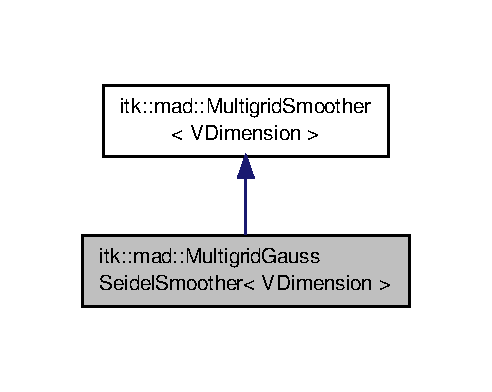
\includegraphics[width=236pt]{classitk_1_1mad_1_1_multigrid_gauss_seidel_smoother__inherit__graph}
\end{center}
\end{figure}


Collaboration diagram for itk\-:\-:mad\-:\-:Multigrid\-Gauss\-Seidel\-Smoother$<$ V\-Dimension $>$\-:
\nopagebreak
\begin{figure}[H]
\begin{center}
\leavevmode
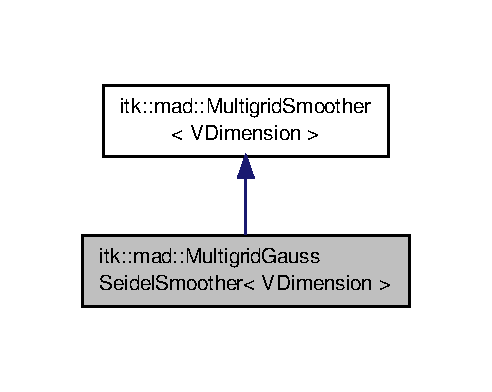
\includegraphics[width=236pt]{classitk_1_1mad_1_1_multigrid_gauss_seidel_smoother__coll__graph}
\end{center}
\end{figure}
\subsection*{Public Types}
\begin{DoxyCompactItemize}
\item 
typedef double \hyperlink{classitk_1_1mad_1_1_multigrid_gauss_seidel_smoother_a317b3e06f245f2953ea8a6bb2fe01500}{Precision}
\item 
\hypertarget{classitk_1_1mad_1_1_multigrid_gauss_seidel_smoother_a7ea983c1815cfd251c9b027ae5b67c96}{typedef \\*
\hyperlink{classitk_1_1mad_1_1_multigrid_gauss_seidel_smoother}{Multigrid\-Gauss\-Seidel\-Smoother} {\bfseries Self}}\label{classitk_1_1mad_1_1_multigrid_gauss_seidel_smoother_a7ea983c1815cfd251c9b027ae5b67c96}

\item 
\hypertarget{classitk_1_1mad_1_1_multigrid_gauss_seidel_smoother_a1a75d5f5179b5c19d8cea51945e8a305}{typedef \hyperlink{class_image}{Image}$<$ \hyperlink{classitk_1_1mad_1_1_multigrid_gauss_seidel_smoother_a317b3e06f245f2953ea8a6bb2fe01500}{Precision}, \\*
V\-Dimension $>$ {\bfseries Image\-Type}}\label{classitk_1_1mad_1_1_multigrid_gauss_seidel_smoother_a1a75d5f5179b5c19d8cea51945e8a305}

\item 
\hypertarget{classitk_1_1mad_1_1_multigrid_gauss_seidel_smoother_af9f0888d73a32ebee321962a846ccc5b}{typedef Neighborhood\\*
$<$ \hyperlink{classitk_1_1mad_1_1_multigrid_gauss_seidel_smoother_a317b3e06f245f2953ea8a6bb2fe01500}{Precision}, V\-Dimension $>$ {\bfseries Stencil\-Type}}\label{classitk_1_1mad_1_1_multigrid_gauss_seidel_smoother_af9f0888d73a32ebee321962a846ccc5b}

\item 
\hypertarget{classitk_1_1mad_1_1_multigrid_gauss_seidel_smoother_a28861e612bc8d787bb300024b77da55a}{typedef \hyperlink{classitk_1_1mad_1_1_stencil_image}{Stencil\-Image}\\*
$<$ \hyperlink{classitk_1_1mad_1_1_multigrid_gauss_seidel_smoother_a317b3e06f245f2953ea8a6bb2fe01500}{Precision}, V\-Dimension $>$ {\bfseries Stencil\-Image\-Type}}\label{classitk_1_1mad_1_1_multigrid_gauss_seidel_smoother_a28861e612bc8d787bb300024b77da55a}

\item 
\hypertarget{classitk_1_1mad_1_1_multigrid_gauss_seidel_smoother_a28c14e90449ab800803266d8a2f22bb6}{typedef Image\-Region$<$ V\-Dimension $>$ {\bfseries Image\-Region\-Type}}\label{classitk_1_1mad_1_1_multigrid_gauss_seidel_smoother_a28c14e90449ab800803266d8a2f22bb6}

\item 
\hypertarget{classitk_1_1mad_1_1_multigrid_gauss_seidel_smoother_a8c6d141ea223ed36e49c478581bd46be}{typedef Image\-Type\-::\-Spacing\-Type {\bfseries Spacing\-Type}}\label{classitk_1_1mad_1_1_multigrid_gauss_seidel_smoother_a8c6d141ea223ed36e49c478581bd46be}

\item 
\hypertarget{classitk_1_1mad_1_1_multigrid_gauss_seidel_smoother_a10a527038fbe1a15719bee4eb6964e7a}{typedef Image\-Type\-::\-Size\-Type {\bfseries Size\-Type}}\label{classitk_1_1mad_1_1_multigrid_gauss_seidel_smoother_a10a527038fbe1a15719bee4eb6964e7a}

\item 
\hypertarget{classitk_1_1mad_1_1_multigrid_gauss_seidel_smoother_abc4ba9247d66a1f715240e5bf092ddb8}{typedef Image\-Type\-::\-Index\-Type {\bfseries Index\-Type}}\label{classitk_1_1mad_1_1_multigrid_gauss_seidel_smoother_abc4ba9247d66a1f715240e5bf092ddb8}

\item 
\hypertarget{classitk_1_1mad_1_1_multigrid_gauss_seidel_smoother_af282c18a17a2d1f95304aea786cc5a9f}{typedef Image\-Type\-::\-Offset\-Type {\bfseries Offset\-Type}}\label{classitk_1_1mad_1_1_multigrid_gauss_seidel_smoother_af282c18a17a2d1f95304aea786cc5a9f}

\item 
\hypertarget{classitk_1_1mad_1_1_multigrid_gauss_seidel_smoother_a6bc4af1c0d41e026330ccb9acdff2794}{typedef std\-::list$<$ Offset\-Type $>$ {\bfseries Offset\-List\-Type}}\label{classitk_1_1mad_1_1_multigrid_gauss_seidel_smoother_a6bc4af1c0d41e026330ccb9acdff2794}

\end{DoxyCompactItemize}
\subsection*{Public Member Functions}
\begin{DoxyCompactItemize}
\item 
Image\-Type\-::\-Pointer \hyperlink{classitk_1_1mad_1_1_multigrid_gauss_seidel_smoother_a4c4efcf4c1d207014ec08a58f05cbea4}{Single\-Iteration} (const \hyperlink{class_image}{Image\-Type} $\ast$input\-Image, const \hyperlink{class_image}{Image\-Type} $\ast$rhs\-Image, const \hyperlink{classitk_1_1mad_1_1_stencil_image}{Stencil\-Image\-Type} $\ast$matrix\-Image) const 
\item 
Image\-Type\-::\-Pointer \hyperlink{classitk_1_1mad_1_1_multigrid_gauss_seidel_smoother_a918b18641139d9e0cb99f97e751e2103}{Compute\-Residual} (const \hyperlink{class_image}{Image\-Type} $\ast$input\-Image, const \hyperlink{class_image}{Image\-Type} $\ast$rhs\-Image, const \hyperlink{classitk_1_1mad_1_1_stencil_image}{Stencil\-Image\-Type} $\ast$matrix\-Image) const 
\item 
\hyperlink{classitk_1_1mad_1_1_multigrid_gauss_seidel_smoother_a5ac6b70226e4af8bdfd115ffb52ab5ac}{Multigrid\-Gauss\-Seidel\-Smoother} ()
\item 
\hyperlink{classitk_1_1mad_1_1_multigrid_gauss_seidel_smoother_af85c0d56057fe68365a6b6b4c45f7698}{$\sim$\-Multigrid\-Gauss\-Seidel\-Smoother} ()
\end{DoxyCompactItemize}


\subsection{Detailed Description}
\subsubsection*{template$<$unsigned int V\-Dimension$>$class itk\-::mad\-::\-Multigrid\-Gauss\-Seidel\-Smoother$<$ V\-Dimension $>$}

Gauss Seidel smoother implementation; it is a derived class of \hyperlink{classitk_1_1mad_1_1_multigrid_smoother}{Multigrid\-Smoother}. It internally uses a lexicographic ordering of the points. 

\begin{DoxyAuthor}{Author}
Antonello Gerbi 
\end{DoxyAuthor}


Definition at line 42 of file itk\-Multigrid\-Gauss\-Seidel\-Smoother.\-h.



\subsection{Member Typedef Documentation}
\hypertarget{classitk_1_1mad_1_1_multigrid_gauss_seidel_smoother_a317b3e06f245f2953ea8a6bb2fe01500}{\index{itk\-::mad\-::\-Multigrid\-Gauss\-Seidel\-Smoother@{itk\-::mad\-::\-Multigrid\-Gauss\-Seidel\-Smoother}!Precision@{Precision}}
\index{Precision@{Precision}!itk::mad::MultigridGaussSeidelSmoother@{itk\-::mad\-::\-Multigrid\-Gauss\-Seidel\-Smoother}}
\subsubsection[{Precision}]{\setlength{\rightskip}{0pt plus 5cm}template$<$unsigned int V\-Dimension$>$ typedef double {\bf itk\-::mad\-::\-Multigrid\-Gauss\-Seidel\-Smoother}$<$ V\-Dimension $>$\-::{\bf Precision}}}\label{classitk_1_1mad_1_1_multigrid_gauss_seidel_smoother_a317b3e06f245f2953ea8a6bb2fe01500}
Standard class typedefs. 

Definition at line 47 of file itk\-Multigrid\-Gauss\-Seidel\-Smoother.\-h.



\subsection{Constructor \& Destructor Documentation}
\hypertarget{classitk_1_1mad_1_1_multigrid_gauss_seidel_smoother_a5ac6b70226e4af8bdfd115ffb52ab5ac}{\index{itk\-::mad\-::\-Multigrid\-Gauss\-Seidel\-Smoother@{itk\-::mad\-::\-Multigrid\-Gauss\-Seidel\-Smoother}!Multigrid\-Gauss\-Seidel\-Smoother@{Multigrid\-Gauss\-Seidel\-Smoother}}
\index{Multigrid\-Gauss\-Seidel\-Smoother@{Multigrid\-Gauss\-Seidel\-Smoother}!itk::mad::MultigridGaussSeidelSmoother@{itk\-::mad\-::\-Multigrid\-Gauss\-Seidel\-Smoother}}
\subsubsection[{Multigrid\-Gauss\-Seidel\-Smoother}]{\setlength{\rightskip}{0pt plus 5cm}template$<$unsigned int V\-Dimension$>$ {\bf itk\-::mad\-::\-Multigrid\-Gauss\-Seidel\-Smoother}$<$ V\-Dimension $>$\-::{\bf Multigrid\-Gauss\-Seidel\-Smoother} (
\begin{DoxyParamCaption}
{}
\end{DoxyParamCaption}
)}}\label{classitk_1_1mad_1_1_multigrid_gauss_seidel_smoother_a5ac6b70226e4af8bdfd115ffb52ab5ac}
Class constructor 

Definition at line 185 of file itk\-Multigrid\-Gauss\-Seidel\-Smoother.\-hxx.

\hypertarget{classitk_1_1mad_1_1_multigrid_gauss_seidel_smoother_af85c0d56057fe68365a6b6b4c45f7698}{\index{itk\-::mad\-::\-Multigrid\-Gauss\-Seidel\-Smoother@{itk\-::mad\-::\-Multigrid\-Gauss\-Seidel\-Smoother}!$\sim$\-Multigrid\-Gauss\-Seidel\-Smoother@{$\sim$\-Multigrid\-Gauss\-Seidel\-Smoother}}
\index{$\sim$\-Multigrid\-Gauss\-Seidel\-Smoother@{$\sim$\-Multigrid\-Gauss\-Seidel\-Smoother}!itk::mad::MultigridGaussSeidelSmoother@{itk\-::mad\-::\-Multigrid\-Gauss\-Seidel\-Smoother}}
\subsubsection[{$\sim$\-Multigrid\-Gauss\-Seidel\-Smoother}]{\setlength{\rightskip}{0pt plus 5cm}template$<$unsigned int V\-Dimension$>$ {\bf itk\-::mad\-::\-Multigrid\-Gauss\-Seidel\-Smoother}$<$ V\-Dimension $>$\-::$\sim${\bf Multigrid\-Gauss\-Seidel\-Smoother} (
\begin{DoxyParamCaption}
{}
\end{DoxyParamCaption}
)}}\label{classitk_1_1mad_1_1_multigrid_gauss_seidel_smoother_af85c0d56057fe68365a6b6b4c45f7698}
Class destructor. 

Definition at line 193 of file itk\-Multigrid\-Gauss\-Seidel\-Smoother.\-hxx.



\subsection{Member Function Documentation}
\hypertarget{classitk_1_1mad_1_1_multigrid_gauss_seidel_smoother_a918b18641139d9e0cb99f97e751e2103}{\index{itk\-::mad\-::\-Multigrid\-Gauss\-Seidel\-Smoother@{itk\-::mad\-::\-Multigrid\-Gauss\-Seidel\-Smoother}!Compute\-Residual@{Compute\-Residual}}
\index{Compute\-Residual@{Compute\-Residual}!itk::mad::MultigridGaussSeidelSmoother@{itk\-::mad\-::\-Multigrid\-Gauss\-Seidel\-Smoother}}
\subsubsection[{Compute\-Residual}]{\setlength{\rightskip}{0pt plus 5cm}template$<$unsigned int V\-Dimension$>$ {\bf Multigrid\-Gauss\-Seidel\-Smoother}$<$ V\-Dimension $>$\-::Image\-Type\-::\-Pointer {\bf itk\-::mad\-::\-Multigrid\-Gauss\-Seidel\-Smoother}$<$ V\-Dimension $>$\-::Compute\-Residual (
\begin{DoxyParamCaption}
\item[{const {\bf Image\-Type} $\ast$}]{input\-Image, }
\item[{const {\bf Image\-Type} $\ast$}]{rhs\-Image, }
\item[{const {\bf Stencil\-Image\-Type} $\ast$}]{matrix\-Image}
\end{DoxyParamCaption}
) const\hspace{0.3cm}{\ttfamily [virtual]}}}\label{classitk_1_1mad_1_1_multigrid_gauss_seidel_smoother_a918b18641139d9e0cb99f97e751e2103}
Returns the residual $ r = b - A x $, where input\-Image is the term $ x $, rhs\-Image is $ b $, and matrix\-Image the matrix $ A $. 

Implements \hyperlink{classitk_1_1mad_1_1_multigrid_smoother_a7b90d4fbff488ad00ed0bd680913f227}{itk\-::mad\-::\-Multigrid\-Smoother$<$ V\-Dimension $>$}.



Definition at line 117 of file itk\-Multigrid\-Gauss\-Seidel\-Smoother.\-hxx.

\hypertarget{classitk_1_1mad_1_1_multigrid_gauss_seidel_smoother_a4c4efcf4c1d207014ec08a58f05cbea4}{\index{itk\-::mad\-::\-Multigrid\-Gauss\-Seidel\-Smoother@{itk\-::mad\-::\-Multigrid\-Gauss\-Seidel\-Smoother}!Single\-Iteration@{Single\-Iteration}}
\index{Single\-Iteration@{Single\-Iteration}!itk::mad::MultigridGaussSeidelSmoother@{itk\-::mad\-::\-Multigrid\-Gauss\-Seidel\-Smoother}}
\subsubsection[{Single\-Iteration}]{\setlength{\rightskip}{0pt plus 5cm}template$<$unsigned int V\-Dimension$>$ {\bf Multigrid\-Gauss\-Seidel\-Smoother}$<$ V\-Dimension $>$\-::Image\-Type\-::\-Pointer {\bf itk\-::mad\-::\-Multigrid\-Gauss\-Seidel\-Smoother}$<$ V\-Dimension $>$\-::Single\-Iteration (
\begin{DoxyParamCaption}
\item[{const {\bf Image\-Type} $\ast$}]{input\-Image, }
\item[{const {\bf Image\-Type} $\ast$}]{rhs\-Image, }
\item[{const {\bf Stencil\-Image\-Type} $\ast$}]{matrix\-Image}
\end{DoxyParamCaption}
) const\hspace{0.3cm}{\ttfamily [virtual]}}}\label{classitk_1_1mad_1_1_multigrid_gauss_seidel_smoother_a4c4efcf4c1d207014ec08a58f05cbea4}
Returns the approximated solution to problem $ A x = b$ after one iteration of the smoother, starting with input\-Image as initial guess, rhs\-Image as the right hand side $ b $, and matrix\-Image as matrix $ A $ in Stencil\-Image\-Type format. 

Implements \hyperlink{classitk_1_1mad_1_1_multigrid_smoother_a1163b85294e86ee03990020bc81fe465}{itk\-::mad\-::\-Multigrid\-Smoother$<$ V\-Dimension $>$}.



Definition at line 36 of file itk\-Multigrid\-Gauss\-Seidel\-Smoother.\-hxx.



The documentation for this class was generated from the following files\-:\begin{DoxyCompactItemize}
\item 
mad/itk\-Multigrid\-Gauss\-Seidel\-Smoother.\-h\item 
mad/itk\-Multigrid\-Gauss\-Seidel\-Smoother.\-hxx\end{DoxyCompactItemize}

\hypertarget{classitk_1_1mad_1_1_multigrid_smoother}{\section{itk\-:\-:mad\-:\-:Multigrid\-Smoother$<$ V\-Dimension $>$ Class Template Reference}
\label{classitk_1_1mad_1_1_multigrid_smoother}\index{itk\-::mad\-::\-Multigrid\-Smoother$<$ V\-Dimension $>$@{itk\-::mad\-::\-Multigrid\-Smoother$<$ V\-Dimension $>$}}
}


Base class for a generic smoother. The derived class has to provide an implementation of the methods Single\-Iteration and Compute\-Residual defined in the public section, which refer to the problem.  




{\ttfamily \#include $<$itk\-Multigrid\-Smoother.\-h$>$}



Inheritance diagram for itk\-:\-:mad\-:\-:Multigrid\-Smoother$<$ V\-Dimension $>$\-:
\nopagebreak
\begin{figure}[H]
\begin{center}
\leavevmode
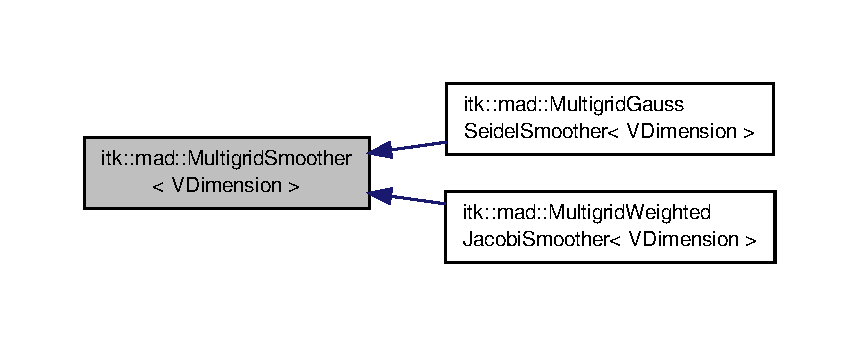
\includegraphics[width=350pt]{classitk_1_1mad_1_1_multigrid_smoother__inherit__graph}
\end{center}
\end{figure}
\subsection*{Public Types}
\begin{DoxyCompactItemize}
\item 
typedef double \hyperlink{classitk_1_1mad_1_1_multigrid_smoother_a23c762f89a3b1509f0a64cfd42e82427}{Precision}
\item 
\hypertarget{classitk_1_1mad_1_1_multigrid_smoother_ad1261cf9fae2f872d29767e15bfcd0b0}{typedef \hyperlink{classitk_1_1mad_1_1_multigrid_smoother}{Multigrid\-Smoother} {\bfseries Self}}\label{classitk_1_1mad_1_1_multigrid_smoother_ad1261cf9fae2f872d29767e15bfcd0b0}

\item 
\hypertarget{classitk_1_1mad_1_1_multigrid_smoother_adf26b2e9c62c3bd6106b30f0b0f1d643}{typedef \hyperlink{class_image}{Image}$<$ \hyperlink{classitk_1_1mad_1_1_multigrid_smoother_a23c762f89a3b1509f0a64cfd42e82427}{Precision}, \\*
V\-Dimension $>$ {\bfseries Image\-Type}}\label{classitk_1_1mad_1_1_multigrid_smoother_adf26b2e9c62c3bd6106b30f0b0f1d643}

\item 
\hypertarget{classitk_1_1mad_1_1_multigrid_smoother_ad3c31fa3229d0e0f9c7db051dd624475}{typedef \hyperlink{classitk_1_1mad_1_1_stencil_image}{Stencil\-Image}\\*
$<$ \hyperlink{classitk_1_1mad_1_1_multigrid_smoother_a23c762f89a3b1509f0a64cfd42e82427}{Precision}, V\-Dimension $>$ {\bfseries Stencil\-Image\-Type}}\label{classitk_1_1mad_1_1_multigrid_smoother_ad3c31fa3229d0e0f9c7db051dd624475}

\end{DoxyCompactItemize}
\subsection*{Public Member Functions}
\begin{DoxyCompactItemize}
\item 
virtual Image\-Type\-::\-Pointer \hyperlink{classitk_1_1mad_1_1_multigrid_smoother_a1163b85294e86ee03990020bc81fe465}{Single\-Iteration} (const \hyperlink{class_image}{Image\-Type} $\ast$input\-Image, const \hyperlink{class_image}{Image\-Type} $\ast$rhs\-Image, const \hyperlink{classitk_1_1mad_1_1_stencil_image}{Stencil\-Image\-Type} $\ast$matrix\-Image) const =0
\item 
virtual Image\-Type\-::\-Pointer \hyperlink{classitk_1_1mad_1_1_multigrid_smoother_a7b90d4fbff488ad00ed0bd680913f227}{Compute\-Residual} (const \hyperlink{class_image}{Image\-Type} $\ast$input\-Image, const \hyperlink{class_image}{Image\-Type} $\ast$rhs\-Image, const \hyperlink{classitk_1_1mad_1_1_stencil_image}{Stencil\-Image\-Type} $\ast$matrix\-Image) const =0
\item 
\hyperlink{classitk_1_1mad_1_1_multigrid_smoother_a4b022644c398078c92ac26323df6eae4}{Multigrid\-Smoother} ()
\item 
virtual \hyperlink{classitk_1_1mad_1_1_multigrid_smoother_a853383223dfa14c417e2788d1a3558fd}{$\sim$\-Multigrid\-Smoother} ()
\end{DoxyCompactItemize}


\subsection{Detailed Description}
\subsubsection*{template$<$unsigned int V\-Dimension$>$class itk\-::mad\-::\-Multigrid\-Smoother$<$ V\-Dimension $>$}

Base class for a generic smoother. The derived class has to provide an implementation of the methods Single\-Iteration and Compute\-Residual defined in the public section, which refer to the problem. 

\[ A x = b \]

\begin{DoxyAuthor}{Author}
Antonello Gerbi 
\end{DoxyAuthor}


Definition at line 45 of file itk\-Multigrid\-Smoother.\-h.



\subsection{Member Typedef Documentation}
\hypertarget{classitk_1_1mad_1_1_multigrid_smoother_a23c762f89a3b1509f0a64cfd42e82427}{\index{itk\-::mad\-::\-Multigrid\-Smoother@{itk\-::mad\-::\-Multigrid\-Smoother}!Precision@{Precision}}
\index{Precision@{Precision}!itk::mad::MultigridSmoother@{itk\-::mad\-::\-Multigrid\-Smoother}}
\subsubsection[{Precision}]{\setlength{\rightskip}{0pt plus 5cm}template$<$unsigned int V\-Dimension$>$ typedef double {\bf itk\-::mad\-::\-Multigrid\-Smoother}$<$ V\-Dimension $>$\-::{\bf Precision}}}\label{classitk_1_1mad_1_1_multigrid_smoother_a23c762f89a3b1509f0a64cfd42e82427}
Standard class typedefs. 

Definition at line 50 of file itk\-Multigrid\-Smoother.\-h.



\subsection{Constructor \& Destructor Documentation}
\hypertarget{classitk_1_1mad_1_1_multigrid_smoother_a4b022644c398078c92ac26323df6eae4}{\index{itk\-::mad\-::\-Multigrid\-Smoother@{itk\-::mad\-::\-Multigrid\-Smoother}!Multigrid\-Smoother@{Multigrid\-Smoother}}
\index{Multigrid\-Smoother@{Multigrid\-Smoother}!itk::mad::MultigridSmoother@{itk\-::mad\-::\-Multigrid\-Smoother}}
\subsubsection[{Multigrid\-Smoother}]{\setlength{\rightskip}{0pt plus 5cm}template$<$unsigned int V\-Dimension$>$ {\bf itk\-::mad\-::\-Multigrid\-Smoother}$<$ V\-Dimension $>$\-::{\bf Multigrid\-Smoother} (
\begin{DoxyParamCaption}
{}
\end{DoxyParamCaption}
)}}\label{classitk_1_1mad_1_1_multigrid_smoother_a4b022644c398078c92ac26323df6eae4}
Class constructor 

Definition at line 80 of file itk\-Multigrid\-Smoother.\-h.

\hypertarget{classitk_1_1mad_1_1_multigrid_smoother_a853383223dfa14c417e2788d1a3558fd}{\index{itk\-::mad\-::\-Multigrid\-Smoother@{itk\-::mad\-::\-Multigrid\-Smoother}!$\sim$\-Multigrid\-Smoother@{$\sim$\-Multigrid\-Smoother}}
\index{$\sim$\-Multigrid\-Smoother@{$\sim$\-Multigrid\-Smoother}!itk::mad::MultigridSmoother@{itk\-::mad\-::\-Multigrid\-Smoother}}
\subsubsection[{$\sim$\-Multigrid\-Smoother}]{\setlength{\rightskip}{0pt plus 5cm}template$<$unsigned int V\-Dimension$>$ {\bf itk\-::mad\-::\-Multigrid\-Smoother}$<$ V\-Dimension $>$\-::$\sim${\bf Multigrid\-Smoother} (
\begin{DoxyParamCaption}
{}
\end{DoxyParamCaption}
)\hspace{0.3cm}{\ttfamily [virtual]}}}\label{classitk_1_1mad_1_1_multigrid_smoother_a853383223dfa14c417e2788d1a3558fd}
Class destructor. 

Definition at line 84 of file itk\-Multigrid\-Smoother.\-h.



\subsection{Member Function Documentation}
\hypertarget{classitk_1_1mad_1_1_multigrid_smoother_a7b90d4fbff488ad00ed0bd680913f227}{\index{itk\-::mad\-::\-Multigrid\-Smoother@{itk\-::mad\-::\-Multigrid\-Smoother}!Compute\-Residual@{Compute\-Residual}}
\index{Compute\-Residual@{Compute\-Residual}!itk::mad::MultigridSmoother@{itk\-::mad\-::\-Multigrid\-Smoother}}
\subsubsection[{Compute\-Residual}]{\setlength{\rightskip}{0pt plus 5cm}template$<$unsigned int V\-Dimension$>$ virtual Image\-Type\-::\-Pointer {\bf itk\-::mad\-::\-Multigrid\-Smoother}$<$ V\-Dimension $>$\-::Compute\-Residual (
\begin{DoxyParamCaption}
\item[{const {\bf Image\-Type} $\ast$}]{input\-Image, }
\item[{const {\bf Image\-Type} $\ast$}]{rhs\-Image, }
\item[{const {\bf Stencil\-Image\-Type} $\ast$}]{matrix\-Image}
\end{DoxyParamCaption}
) const\hspace{0.3cm}{\ttfamily [pure virtual]}}}\label{classitk_1_1mad_1_1_multigrid_smoother_a7b90d4fbff488ad00ed0bd680913f227}
Returns the residual $ r = b - A x $, where input\-Image is the term $ x $, rhs\-Image is $ b $, and matrix\-Image the matrix $ A $. 

Implemented in \hyperlink{classitk_1_1mad_1_1_multigrid_gauss_seidel_smoother_a918b18641139d9e0cb99f97e751e2103}{itk\-::mad\-::\-Multigrid\-Gauss\-Seidel\-Smoother$<$ V\-Dimension $>$}, and \hyperlink{classitk_1_1mad_1_1_multigrid_weighted_jacobi_smoother_ac624a5ecbf37dc87a76709be747af2eb}{itk\-::mad\-::\-Multigrid\-Weighted\-Jacobi\-Smoother$<$ V\-Dimension $>$}.

\hypertarget{classitk_1_1mad_1_1_multigrid_smoother_a1163b85294e86ee03990020bc81fe465}{\index{itk\-::mad\-::\-Multigrid\-Smoother@{itk\-::mad\-::\-Multigrid\-Smoother}!Single\-Iteration@{Single\-Iteration}}
\index{Single\-Iteration@{Single\-Iteration}!itk::mad::MultigridSmoother@{itk\-::mad\-::\-Multigrid\-Smoother}}
\subsubsection[{Single\-Iteration}]{\setlength{\rightskip}{0pt plus 5cm}template$<$unsigned int V\-Dimension$>$ virtual Image\-Type\-::\-Pointer {\bf itk\-::mad\-::\-Multigrid\-Smoother}$<$ V\-Dimension $>$\-::Single\-Iteration (
\begin{DoxyParamCaption}
\item[{const {\bf Image\-Type} $\ast$}]{input\-Image, }
\item[{const {\bf Image\-Type} $\ast$}]{rhs\-Image, }
\item[{const {\bf Stencil\-Image\-Type} $\ast$}]{matrix\-Image}
\end{DoxyParamCaption}
) const\hspace{0.3cm}{\ttfamily [pure virtual]}}}\label{classitk_1_1mad_1_1_multigrid_smoother_a1163b85294e86ee03990020bc81fe465}
Returns the approximated solution to problem $ A x = b$ after one iteration of the smoother, starting with input\-Image as initial guess, rhs\-Image as the right hand side $ b $, and matrix\-Image as matrix $ A $ in Stencil\-Image\-Type format. 

Implemented in \hyperlink{classitk_1_1mad_1_1_multigrid_weighted_jacobi_smoother_abff75c371a2ca2b85c1715df83eb2265}{itk\-::mad\-::\-Multigrid\-Weighted\-Jacobi\-Smoother$<$ V\-Dimension $>$}, and \hyperlink{classitk_1_1mad_1_1_multigrid_gauss_seidel_smoother_a4c4efcf4c1d207014ec08a58f05cbea4}{itk\-::mad\-::\-Multigrid\-Gauss\-Seidel\-Smoother$<$ V\-Dimension $>$}.



The documentation for this class was generated from the following file\-:\begin{DoxyCompactItemize}
\item 
mad/itk\-Multigrid\-Smoother.\-h\end{DoxyCompactItemize}

\hypertarget{classitk_1_1mad_1_1_multigrid_weighted_jacobi_smoother}{\section{itk\-:\-:mad\-:\-:Multigrid\-Weighted\-Jacobi\-Smoother$<$ V\-Dimension $>$ Class Template Reference}
\label{classitk_1_1mad_1_1_multigrid_weighted_jacobi_smoother}\index{itk\-::mad\-::\-Multigrid\-Weighted\-Jacobi\-Smoother$<$ V\-Dimension $>$@{itk\-::mad\-::\-Multigrid\-Weighted\-Jacobi\-Smoother$<$ V\-Dimension $>$}}
}


Weighted Jacobi smoother implementation; it is a derived class of \hyperlink{classitk_1_1mad_1_1_multigrid_smoother}{Multigrid\-Smoother}, and its constructor can optionally take the weight coefficient as an argument, which otherwise defaults to $ \frac{2}{3} $.  




{\ttfamily \#include $<$itk\-Multigrid\-Weighted\-Jacobi\-Smoother.\-h$>$}



Inheritance diagram for itk\-:\-:mad\-:\-:Multigrid\-Weighted\-Jacobi\-Smoother$<$ V\-Dimension $>$\-:
\nopagebreak
\begin{figure}[H]
\begin{center}
\leavevmode
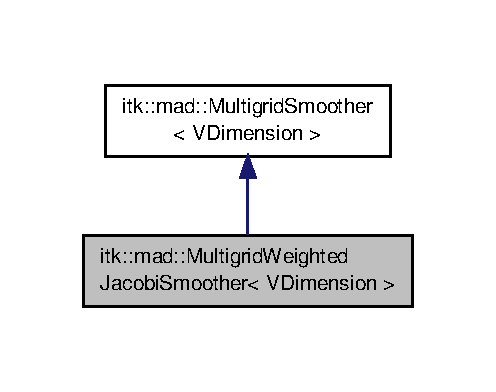
\includegraphics[width=238pt]{classitk_1_1mad_1_1_multigrid_weighted_jacobi_smoother__inherit__graph}
\end{center}
\end{figure}


Collaboration diagram for itk\-:\-:mad\-:\-:Multigrid\-Weighted\-Jacobi\-Smoother$<$ V\-Dimension $>$\-:
\nopagebreak
\begin{figure}[H]
\begin{center}
\leavevmode
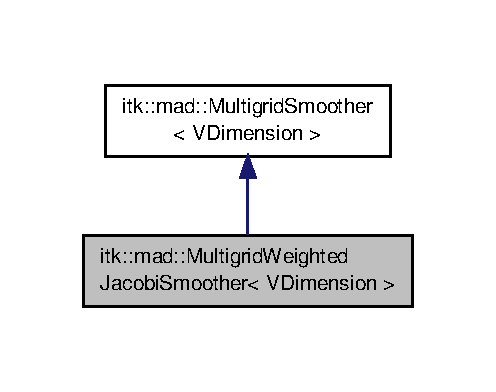
\includegraphics[width=238pt]{classitk_1_1mad_1_1_multigrid_weighted_jacobi_smoother__coll__graph}
\end{center}
\end{figure}
\subsection*{Public Types}
\begin{DoxyCompactItemize}
\item 
typedef double \hyperlink{classitk_1_1mad_1_1_multigrid_weighted_jacobi_smoother_ad82e9067cf76f4ec4bc81b47cb1ff913}{Precision}
\item 
\hypertarget{classitk_1_1mad_1_1_multigrid_weighted_jacobi_smoother_adfd6f96242623fd305eb41b63c4b15fe}{typedef \\*
\hyperlink{classitk_1_1mad_1_1_multigrid_weighted_jacobi_smoother}{Multigrid\-Weighted\-Jacobi\-Smoother} {\bfseries Self}}\label{classitk_1_1mad_1_1_multigrid_weighted_jacobi_smoother_adfd6f96242623fd305eb41b63c4b15fe}

\item 
\hypertarget{classitk_1_1mad_1_1_multigrid_weighted_jacobi_smoother_a4cfc3c97bcdeb6cc2e1b8cb9cd9a438a}{typedef \hyperlink{class_image}{Image}$<$ \hyperlink{classitk_1_1mad_1_1_multigrid_smoother_a23c762f89a3b1509f0a64cfd42e82427}{Precision}, \\*
V\-Dimension $>$ {\bfseries Image\-Type}}\label{classitk_1_1mad_1_1_multigrid_weighted_jacobi_smoother_a4cfc3c97bcdeb6cc2e1b8cb9cd9a438a}

\item 
\hypertarget{classitk_1_1mad_1_1_multigrid_weighted_jacobi_smoother_aed24b462ee32e041e4fdfd7bff82223b}{typedef Neighborhood\\*
$<$ \hyperlink{classitk_1_1mad_1_1_multigrid_smoother_a23c762f89a3b1509f0a64cfd42e82427}{Precision}, V\-Dimension $>$ {\bfseries Stencil\-Type}}\label{classitk_1_1mad_1_1_multigrid_weighted_jacobi_smoother_aed24b462ee32e041e4fdfd7bff82223b}

\item 
\hypertarget{classitk_1_1mad_1_1_multigrid_weighted_jacobi_smoother_ad2472ea4ce3caf2dba673cfc55a2614b}{typedef \hyperlink{classitk_1_1mad_1_1_stencil_image}{Stencil\-Image}\\*
$<$ \hyperlink{classitk_1_1mad_1_1_multigrid_smoother_a23c762f89a3b1509f0a64cfd42e82427}{Precision}, V\-Dimension $>$ {\bfseries Stencil\-Image\-Type}}\label{classitk_1_1mad_1_1_multigrid_weighted_jacobi_smoother_ad2472ea4ce3caf2dba673cfc55a2614b}

\item 
\hypertarget{classitk_1_1mad_1_1_multigrid_weighted_jacobi_smoother_a13c694a23aa665eafe832a2b3428830a}{typedef Image\-Region$<$ V\-Dimension $>$ {\bfseries Image\-Region\-Type}}\label{classitk_1_1mad_1_1_multigrid_weighted_jacobi_smoother_a13c694a23aa665eafe832a2b3428830a}

\item 
\hypertarget{classitk_1_1mad_1_1_multigrid_weighted_jacobi_smoother_ab19da6dfa190f7549149067b351b8898}{typedef Image\-Type\-::\-Spacing\-Type {\bfseries Spacing\-Type}}\label{classitk_1_1mad_1_1_multigrid_weighted_jacobi_smoother_ab19da6dfa190f7549149067b351b8898}

\item 
\hypertarget{classitk_1_1mad_1_1_multigrid_weighted_jacobi_smoother_a7f096c029943ce9ccf6867b22a1c8c98}{typedef Image\-Type\-::\-Size\-Type {\bfseries Size\-Type}}\label{classitk_1_1mad_1_1_multigrid_weighted_jacobi_smoother_a7f096c029943ce9ccf6867b22a1c8c98}

\item 
\hypertarget{classitk_1_1mad_1_1_multigrid_weighted_jacobi_smoother_aa10b4b75946083bfed98cfabb482edb4}{typedef Image\-Type\-::\-Index\-Type {\bfseries Index\-Type}}\label{classitk_1_1mad_1_1_multigrid_weighted_jacobi_smoother_aa10b4b75946083bfed98cfabb482edb4}

\item 
\hypertarget{classitk_1_1mad_1_1_multigrid_weighted_jacobi_smoother_afac53099b5c6f7e1bbb8871c7198f6ed}{typedef Image\-Type\-::\-Offset\-Type {\bfseries Offset\-Type}}\label{classitk_1_1mad_1_1_multigrid_weighted_jacobi_smoother_afac53099b5c6f7e1bbb8871c7198f6ed}

\item 
\hypertarget{classitk_1_1mad_1_1_multigrid_weighted_jacobi_smoother_abfa185356b748e88292a5d3cc5deae7e}{typedef std\-::list$<$ Offset\-Type $>$ {\bfseries Offset\-List\-Type}}\label{classitk_1_1mad_1_1_multigrid_weighted_jacobi_smoother_abfa185356b748e88292a5d3cc5deae7e}

\end{DoxyCompactItemize}
\subsection*{Public Member Functions}
\begin{DoxyCompactItemize}
\item 
Image\-Type\-::\-Pointer \hyperlink{classitk_1_1mad_1_1_multigrid_weighted_jacobi_smoother_abff75c371a2ca2b85c1715df83eb2265}{Single\-Iteration} (const \hyperlink{class_image}{Image\-Type} $\ast$input\-Image, const \hyperlink{class_image}{Image\-Type} $\ast$rhs\-Image, const \hyperlink{classitk_1_1mad_1_1_stencil_image}{Stencil\-Image\-Type} $\ast$matrix\-Image) const 
\item 
Image\-Type\-::\-Pointer \hyperlink{classitk_1_1mad_1_1_multigrid_weighted_jacobi_smoother_ac624a5ecbf37dc87a76709be747af2eb}{Compute\-Residual} (const \hyperlink{class_image}{Image\-Type} $\ast$input\-Image, const \hyperlink{class_image}{Image\-Type} $\ast$rhs\-Image, const \hyperlink{classitk_1_1mad_1_1_stencil_image}{Stencil\-Image\-Type} $\ast$matrix\-Image) const 
\item 
\hyperlink{classitk_1_1mad_1_1_multigrid_weighted_jacobi_smoother_a314c9b962da90a2a411c9e0c9bf0ed23}{Multigrid\-Weighted\-Jacobi\-Smoother} (\hyperlink{classitk_1_1mad_1_1_multigrid_smoother_a23c762f89a3b1509f0a64cfd42e82427}{Precision} weight)
\item 
\hyperlink{classitk_1_1mad_1_1_multigrid_weighted_jacobi_smoother_a8717f0172e8df6ac83f0eb4923672120}{Multigrid\-Weighted\-Jacobi\-Smoother} ()
\item 
\hyperlink{classitk_1_1mad_1_1_multigrid_weighted_jacobi_smoother_a25bbab372e709486120f71df0f4e9e6c}{$\sim$\-Multigrid\-Weighted\-Jacobi\-Smoother} ()
\end{DoxyCompactItemize}


\subsection{Detailed Description}
\subsubsection*{template$<$unsigned int V\-Dimension$>$class itk\-::mad\-::\-Multigrid\-Weighted\-Jacobi\-Smoother$<$ V\-Dimension $>$}

Weighted Jacobi smoother implementation; it is a derived class of \hyperlink{classitk_1_1mad_1_1_multigrid_smoother}{Multigrid\-Smoother}, and its constructor can optionally take the weight coefficient as an argument, which otherwise defaults to $ \frac{2}{3} $. 

\begin{DoxyAuthor}{Author}
Antonello Gerbi 
\end{DoxyAuthor}


Definition at line 43 of file itk\-Multigrid\-Weighted\-Jacobi\-Smoother.\-h.



\subsection{Member Typedef Documentation}
\hypertarget{classitk_1_1mad_1_1_multigrid_weighted_jacobi_smoother_ad82e9067cf76f4ec4bc81b47cb1ff913}{\index{itk\-::mad\-::\-Multigrid\-Weighted\-Jacobi\-Smoother@{itk\-::mad\-::\-Multigrid\-Weighted\-Jacobi\-Smoother}!Precision@{Precision}}
\index{Precision@{Precision}!itk::mad::MultigridWeightedJacobiSmoother@{itk\-::mad\-::\-Multigrid\-Weighted\-Jacobi\-Smoother}}
\subsubsection[{Precision}]{\setlength{\rightskip}{0pt plus 5cm}template$<$unsigned int V\-Dimension$>$ typedef double {\bf itk\-::mad\-::\-Multigrid\-Weighted\-Jacobi\-Smoother}$<$ V\-Dimension $>$\-::{\bf Precision}}}\label{classitk_1_1mad_1_1_multigrid_weighted_jacobi_smoother_ad82e9067cf76f4ec4bc81b47cb1ff913}
Standard class typedefs. 

Definition at line 48 of file itk\-Multigrid\-Weighted\-Jacobi\-Smoother.\-h.



\subsection{Constructor \& Destructor Documentation}
\hypertarget{classitk_1_1mad_1_1_multigrid_weighted_jacobi_smoother_a314c9b962da90a2a411c9e0c9bf0ed23}{\index{itk\-::mad\-::\-Multigrid\-Weighted\-Jacobi\-Smoother@{itk\-::mad\-::\-Multigrid\-Weighted\-Jacobi\-Smoother}!Multigrid\-Weighted\-Jacobi\-Smoother@{Multigrid\-Weighted\-Jacobi\-Smoother}}
\index{Multigrid\-Weighted\-Jacobi\-Smoother@{Multigrid\-Weighted\-Jacobi\-Smoother}!itk::mad::MultigridWeightedJacobiSmoother@{itk\-::mad\-::\-Multigrid\-Weighted\-Jacobi\-Smoother}}
\subsubsection[{Multigrid\-Weighted\-Jacobi\-Smoother}]{\setlength{\rightskip}{0pt plus 5cm}template$<$unsigned int V\-Dimension$>$ {\bf itk\-::mad\-::\-Multigrid\-Weighted\-Jacobi\-Smoother}$<$ V\-Dimension $>$\-::{\bf Multigrid\-Weighted\-Jacobi\-Smoother} (
\begin{DoxyParamCaption}
\item[{{\bf Precision}}]{weight}
\end{DoxyParamCaption}
)}}\label{classitk_1_1mad_1_1_multigrid_weighted_jacobi_smoother_a314c9b962da90a2a411c9e0c9bf0ed23}
Class constructor. 

Definition at line 176 of file itk\-Multigrid\-Weighted\-Jacobi\-Smoother.\-hxx.

\hypertarget{classitk_1_1mad_1_1_multigrid_weighted_jacobi_smoother_a8717f0172e8df6ac83f0eb4923672120}{\index{itk\-::mad\-::\-Multigrid\-Weighted\-Jacobi\-Smoother@{itk\-::mad\-::\-Multigrid\-Weighted\-Jacobi\-Smoother}!Multigrid\-Weighted\-Jacobi\-Smoother@{Multigrid\-Weighted\-Jacobi\-Smoother}}
\index{Multigrid\-Weighted\-Jacobi\-Smoother@{Multigrid\-Weighted\-Jacobi\-Smoother}!itk::mad::MultigridWeightedJacobiSmoother@{itk\-::mad\-::\-Multigrid\-Weighted\-Jacobi\-Smoother}}
\subsubsection[{Multigrid\-Weighted\-Jacobi\-Smoother}]{\setlength{\rightskip}{0pt plus 5cm}template$<$unsigned int V\-Dimension$>$ {\bf itk\-::mad\-::\-Multigrid\-Weighted\-Jacobi\-Smoother}$<$ V\-Dimension $>$\-::{\bf Multigrid\-Weighted\-Jacobi\-Smoother} (
\begin{DoxyParamCaption}
{}
\end{DoxyParamCaption}
)}}\label{classitk_1_1mad_1_1_multigrid_weighted_jacobi_smoother_a8717f0172e8df6ac83f0eb4923672120}
Class contructor, with default weight $ \frac{2}{3} $. 

Definition at line 186 of file itk\-Multigrid\-Weighted\-Jacobi\-Smoother.\-hxx.

\hypertarget{classitk_1_1mad_1_1_multigrid_weighted_jacobi_smoother_a25bbab372e709486120f71df0f4e9e6c}{\index{itk\-::mad\-::\-Multigrid\-Weighted\-Jacobi\-Smoother@{itk\-::mad\-::\-Multigrid\-Weighted\-Jacobi\-Smoother}!$\sim$\-Multigrid\-Weighted\-Jacobi\-Smoother@{$\sim$\-Multigrid\-Weighted\-Jacobi\-Smoother}}
\index{$\sim$\-Multigrid\-Weighted\-Jacobi\-Smoother@{$\sim$\-Multigrid\-Weighted\-Jacobi\-Smoother}!itk::mad::MultigridWeightedJacobiSmoother@{itk\-::mad\-::\-Multigrid\-Weighted\-Jacobi\-Smoother}}
\subsubsection[{$\sim$\-Multigrid\-Weighted\-Jacobi\-Smoother}]{\setlength{\rightskip}{0pt plus 5cm}template$<$unsigned int V\-Dimension$>$ {\bf itk\-::mad\-::\-Multigrid\-Weighted\-Jacobi\-Smoother}$<$ V\-Dimension $>$\-::$\sim${\bf Multigrid\-Weighted\-Jacobi\-Smoother} (
\begin{DoxyParamCaption}
{}
\end{DoxyParamCaption}
)}}\label{classitk_1_1mad_1_1_multigrid_weighted_jacobi_smoother_a25bbab372e709486120f71df0f4e9e6c}
Class destructor. 

Definition at line 196 of file itk\-Multigrid\-Weighted\-Jacobi\-Smoother.\-hxx.



\subsection{Member Function Documentation}
\hypertarget{classitk_1_1mad_1_1_multigrid_weighted_jacobi_smoother_ac624a5ecbf37dc87a76709be747af2eb}{\index{itk\-::mad\-::\-Multigrid\-Weighted\-Jacobi\-Smoother@{itk\-::mad\-::\-Multigrid\-Weighted\-Jacobi\-Smoother}!Compute\-Residual@{Compute\-Residual}}
\index{Compute\-Residual@{Compute\-Residual}!itk::mad::MultigridWeightedJacobiSmoother@{itk\-::mad\-::\-Multigrid\-Weighted\-Jacobi\-Smoother}}
\subsubsection[{Compute\-Residual}]{\setlength{\rightskip}{0pt plus 5cm}template$<$unsigned int V\-Dimension$>$ {\bf Multigrid\-Weighted\-Jacobi\-Smoother}$<$ V\-Dimension $>$\-::Image\-Type\-::\-Pointer {\bf itk\-::mad\-::\-Multigrid\-Weighted\-Jacobi\-Smoother}$<$ V\-Dimension $>$\-::Compute\-Residual (
\begin{DoxyParamCaption}
\item[{const {\bf Image\-Type} $\ast$}]{input\-Image, }
\item[{const {\bf Image\-Type} $\ast$}]{rhs\-Image, }
\item[{const {\bf Stencil\-Image\-Type} $\ast$}]{matrix\-Image}
\end{DoxyParamCaption}
) const\hspace{0.3cm}{\ttfamily [virtual]}}}\label{classitk_1_1mad_1_1_multigrid_weighted_jacobi_smoother_ac624a5ecbf37dc87a76709be747af2eb}
Returns the residual $ r = b - A x $, where input\-Image is the term $ x $, rhs\-Image is $ b $, and matrix\-Image the matrix $ A $. 

Implements \hyperlink{classitk_1_1mad_1_1_multigrid_smoother_a7b90d4fbff488ad00ed0bd680913f227}{itk\-::mad\-::\-Multigrid\-Smoother$<$ V\-Dimension $>$}.



Definition at line 108 of file itk\-Multigrid\-Weighted\-Jacobi\-Smoother.\-hxx.

\hypertarget{classitk_1_1mad_1_1_multigrid_weighted_jacobi_smoother_abff75c371a2ca2b85c1715df83eb2265}{\index{itk\-::mad\-::\-Multigrid\-Weighted\-Jacobi\-Smoother@{itk\-::mad\-::\-Multigrid\-Weighted\-Jacobi\-Smoother}!Single\-Iteration@{Single\-Iteration}}
\index{Single\-Iteration@{Single\-Iteration}!itk::mad::MultigridWeightedJacobiSmoother@{itk\-::mad\-::\-Multigrid\-Weighted\-Jacobi\-Smoother}}
\subsubsection[{Single\-Iteration}]{\setlength{\rightskip}{0pt plus 5cm}template$<$unsigned int V\-Dimension$>$ {\bf Multigrid\-Weighted\-Jacobi\-Smoother}$<$ V\-Dimension $>$\-::Image\-Type\-::\-Pointer {\bf itk\-::mad\-::\-Multigrid\-Weighted\-Jacobi\-Smoother}$<$ V\-Dimension $>$\-::Single\-Iteration (
\begin{DoxyParamCaption}
\item[{const {\bf Image\-Type} $\ast$}]{input\-Image, }
\item[{const {\bf Image\-Type} $\ast$}]{rhs\-Image, }
\item[{const {\bf Stencil\-Image\-Type} $\ast$}]{matrix\-Image}
\end{DoxyParamCaption}
) const\hspace{0.3cm}{\ttfamily [virtual]}}}\label{classitk_1_1mad_1_1_multigrid_weighted_jacobi_smoother_abff75c371a2ca2b85c1715df83eb2265}
Returns the approximated solution to problem $ A x = b$ after one iteration of the smoother, starting with input\-Image as initial guess, rhs\-Image as the right hand side $ b $, and matrix\-Image as matrix $ A $ in Stencil\-Image\-Type format. 

Implements \hyperlink{classitk_1_1mad_1_1_multigrid_smoother_a1163b85294e86ee03990020bc81fe465}{itk\-::mad\-::\-Multigrid\-Smoother$<$ V\-Dimension $>$}.



Definition at line 36 of file itk\-Multigrid\-Weighted\-Jacobi\-Smoother.\-hxx.



The documentation for this class was generated from the following files\-:\begin{DoxyCompactItemize}
\item 
mad/itk\-Multigrid\-Weighted\-Jacobi\-Smoother.\-h\item 
mad/itk\-Multigrid\-Weighted\-Jacobi\-Smoother.\-hxx\end{DoxyCompactItemize}

\hypertarget{classitk_1_1mad_1_1_stencil_image}{\section{itk\-:\-:mad\-:\-:Stencil\-Image$<$ T\-Pixel\-Type, V\-Dimension $>$ Class Template Reference}
\label{classitk_1_1mad_1_1_stencil_image}\index{itk\-::mad\-::\-Stencil\-Image$<$ T\-Pixel\-Type, V\-Dimension $>$@{itk\-::mad\-::\-Stencil\-Image$<$ T\-Pixel\-Type, V\-Dimension $>$}}
}


This class is derived from a specialization of the \hyperlink{class_image}{Image} class, where the Pixel\-Type is defined as a Neighborhood of values\-: it is however templated in order to mimic an \hyperlink{class_image}{Image} class. It is used by the other classes in the I\-T\-K\-Multigrid\-Anisotropic\-Diffusion, and can been interpreted as something similar to a sparse matrix where every row corresponds to a single pixel (i.\-e., a Neighborhood). It also expands the base class, containing a list of active offsets; this is useful in order to easily get the neighbors which need to be visited.  




{\ttfamily \#include $<$itk\-Stencil\-Image.\-h$>$}



Inheritance diagram for itk\-:\-:mad\-:\-:Stencil\-Image$<$ T\-Pixel\-Type, V\-Dimension $>$\-:
\nopagebreak
\begin{figure}[H]
\begin{center}
\leavevmode
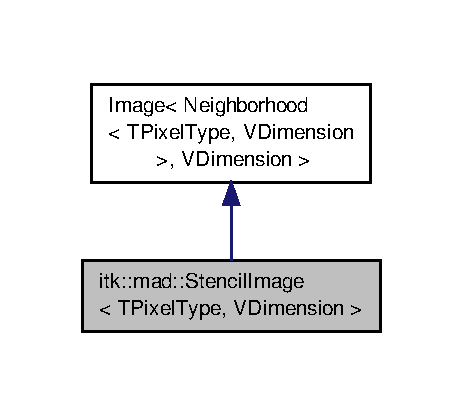
\includegraphics[width=222pt]{classitk_1_1mad_1_1_stencil_image__inherit__graph}
\end{center}
\end{figure}


Collaboration diagram for itk\-:\-:mad\-:\-:Stencil\-Image$<$ T\-Pixel\-Type, V\-Dimension $>$\-:
\nopagebreak
\begin{figure}[H]
\begin{center}
\leavevmode
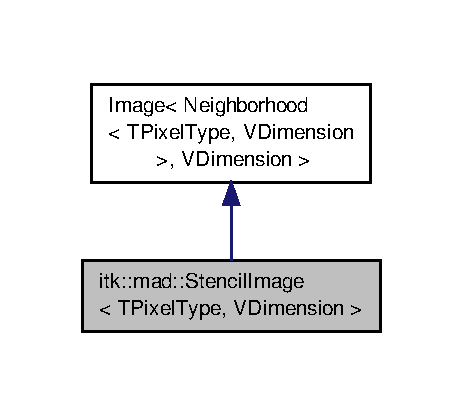
\includegraphics[width=222pt]{classitk_1_1mad_1_1_stencil_image__coll__graph}
\end{center}
\end{figure}
\subsection*{Public Types}
\begin{DoxyCompactItemize}
\item 
typedef \hyperlink{classitk_1_1mad_1_1_stencil_image}{Stencil\-Image} \hyperlink{classitk_1_1mad_1_1_stencil_image_a3cd288ed59c1431bf14b735b995cf58c}{Self}
\item 
\hypertarget{classitk_1_1mad_1_1_stencil_image_aaedf6e494e423e4aba74c26d970c2b1f}{typedef \hyperlink{class_image}{Image}$<$ Neighborhood\\*
$<$ T\-Pixel\-Type, V\-Dimension $>$\\*
, V\-Dimension $>$ {\bfseries Super\-Class}}\label{classitk_1_1mad_1_1_stencil_image_aaedf6e494e423e4aba74c26d970c2b1f}

\item 
\hypertarget{classitk_1_1mad_1_1_stencil_image_ad40004fa579b36db5e85209e1d559fec}{typedef Smart\-Pointer$<$ \hyperlink{classitk_1_1mad_1_1_stencil_image_a3cd288ed59c1431bf14b735b995cf58c}{Self} $>$ {\bfseries Pointer}}\label{classitk_1_1mad_1_1_stencil_image_ad40004fa579b36db5e85209e1d559fec}

\item 
\hypertarget{classitk_1_1mad_1_1_stencil_image_a36d23e924004565c1294bc8c68d601de}{typedef Smart\-Pointer$<$ const \hyperlink{classitk_1_1mad_1_1_stencil_image_a3cd288ed59c1431bf14b735b995cf58c}{Self} $>$ {\bfseries Const\-Pointer}}\label{classitk_1_1mad_1_1_stencil_image_a36d23e924004565c1294bc8c68d601de}

\item 
\hypertarget{classitk_1_1mad_1_1_stencil_image_ab44e26a599f3e210a5631caefe172732}{typedef Neighborhood\\*
$<$ T\-Pixel\-Type, V\-Dimension $>$ {\bfseries Stencil\-Type}}\label{classitk_1_1mad_1_1_stencil_image_ab44e26a599f3e210a5631caefe172732}

\item 
\hypertarget{classitk_1_1mad_1_1_stencil_image_a5f68ed1c8592a0570a58ac007a509f11}{typedef \hyperlink{class_image}{Image}$<$ T\-Pixel\-Type, \\*
V\-Dimension $>$ {\bfseries Image\-Type}}\label{classitk_1_1mad_1_1_stencil_image_a5f68ed1c8592a0570a58ac007a509f11}

\item 
\hypertarget{classitk_1_1mad_1_1_stencil_image_ab9a05a7d77b7149fb84f5699744f9bae}{typedef Image\-Type\-::\-Offset\-Type {\bfseries Offset\-Type}}\label{classitk_1_1mad_1_1_stencil_image_ab9a05a7d77b7149fb84f5699744f9bae}

\item 
\hypertarget{classitk_1_1mad_1_1_stencil_image_aceb14d8286df6cc90aecfedf018866b2}{typedef std\-::list$<$ Offset\-Type $>$ {\bfseries Offset\-List\-Type}}\label{classitk_1_1mad_1_1_stencil_image_aceb14d8286df6cc90aecfedf018866b2}

\item 
\hypertarget{classitk_1_1mad_1_1_stencil_image_a0198ac532d563c49c83b52dbc5666db9}{typedef Image\-Type\-::\-Size\-Type {\bfseries Size\-Type}}\label{classitk_1_1mad_1_1_stencil_image_a0198ac532d563c49c83b52dbc5666db9}

\end{DoxyCompactItemize}
\subsection*{Public Member Functions}
\begin{DoxyCompactItemize}
\item 
\hyperlink{classitk_1_1mad_1_1_stencil_image_a954e0ebaabb189c36354f82542f3acec}{itk\-New\-Macro} (\hyperlink{classitk_1_1mad_1_1_stencil_image_a3cd288ed59c1431bf14b735b995cf58c}{Self})
\item 
\hyperlink{classitk_1_1mad_1_1_stencil_image_a951543783bd9bdd9074e569fc72c0dca}{itk\-Type\-Macro} (\hyperlink{classitk_1_1mad_1_1_stencil_image}{Stencil\-Image}, \hyperlink{class_image}{Image})
\item 
void \hyperlink{classitk_1_1mad_1_1_stencil_image_a58c14a128e9348f27d64434373d26b90}{Activate\-All\-Offsets} ()
\item 
\hyperlink{classitk_1_1mad_1_1_stencil_image_a7680f0a93498d9f39f303160c457c410}{itk\-Get\-Const\-Macro} (Active\-Offset\-List, Offset\-List\-Type)
\item 
Offset\-List\-Type\-::size\-\_\-type \hyperlink{classitk_1_1mad_1_1_stencil_image_ab783f408069969cebf420730541bb6a4}{Get\-Active\-Offset\-List\-Size} () const 
\item 
\hyperlink{classitk_1_1mad_1_1_stencil_image_abe294bd353e53fcf37cbfb442ae1cfdc}{itk\-Get\-Const\-Macro} (Radius, Size\-Type)
\item 
\hyperlink{classitk_1_1mad_1_1_stencil_image_a053e227d7c8891c5dd2e4a0722977694}{itk\-Set\-Macro} (Radius, Size\-Type)
\end{DoxyCompactItemize}
\subsection*{Protected Member Functions}
\begin{DoxyCompactItemize}
\item 
\hyperlink{classitk_1_1mad_1_1_stencil_image_a5034dab56f499ea99139b4798ed12a19}{Stencil\-Image} ()
\item 
virtual \hyperlink{classitk_1_1mad_1_1_stencil_image_ac8bdf1a707f80129e37a9cf6fcf32650}{$\sim$\-Stencil\-Image} ()
\end{DoxyCompactItemize}


\subsection{Detailed Description}
\subsubsection*{template$<$class T\-Pixel\-Type, unsigned int V\-Dimension$>$class itk\-::mad\-::\-Stencil\-Image$<$ T\-Pixel\-Type, V\-Dimension $>$}

This class is derived from a specialization of the \hyperlink{class_image}{Image} class, where the Pixel\-Type is defined as a Neighborhood of values\-: it is however templated in order to mimic an \hyperlink{class_image}{Image} class. It is used by the other classes in the I\-T\-K\-Multigrid\-Anisotropic\-Diffusion, and can been interpreted as something similar to a sparse matrix where every row corresponds to a single pixel (i.\-e., a Neighborhood). It also expands the base class, containing a list of active offsets; this is useful in order to easily get the neighbors which need to be visited. 

\begin{DoxyAuthor}{Author}
Antonello Gerbi 
\end{DoxyAuthor}


Definition at line 48 of file itk\-Stencil\-Image.\-h.



\subsection{Member Typedef Documentation}
\hypertarget{classitk_1_1mad_1_1_stencil_image_a3cd288ed59c1431bf14b735b995cf58c}{\index{itk\-::mad\-::\-Stencil\-Image@{itk\-::mad\-::\-Stencil\-Image}!Self@{Self}}
\index{Self@{Self}!itk::mad::StencilImage@{itk\-::mad\-::\-Stencil\-Image}}
\subsubsection[{Self}]{\setlength{\rightskip}{0pt plus 5cm}template$<$class T\-Pixel\-Type, unsigned int V\-Dimension$>$ typedef {\bf Stencil\-Image} {\bf itk\-::mad\-::\-Stencil\-Image}$<$ T\-Pixel\-Type, V\-Dimension $>$\-::{\bf Self}}}\label{classitk_1_1mad_1_1_stencil_image_a3cd288ed59c1431bf14b735b995cf58c}
Standard class typedefs. 

Definition at line 53 of file itk\-Stencil\-Image.\-h.



\subsection{Constructor \& Destructor Documentation}
\hypertarget{classitk_1_1mad_1_1_stencil_image_a5034dab56f499ea99139b4798ed12a19}{\index{itk\-::mad\-::\-Stencil\-Image@{itk\-::mad\-::\-Stencil\-Image}!Stencil\-Image@{Stencil\-Image}}
\index{Stencil\-Image@{Stencil\-Image}!itk::mad::StencilImage@{itk\-::mad\-::\-Stencil\-Image}}
\subsubsection[{Stencil\-Image}]{\setlength{\rightskip}{0pt plus 5cm}template$<$class T\-Pixel\-Type , unsigned int V\-Dimension$>$ {\bf itk\-::mad\-::\-Stencil\-Image}$<$ T\-Pixel\-Type, V\-Dimension $>$\-::{\bf Stencil\-Image} (
\begin{DoxyParamCaption}
{}
\end{DoxyParamCaption}
)\hspace{0.3cm}{\ttfamily [protected]}}}\label{classitk_1_1mad_1_1_stencil_image_a5034dab56f499ea99139b4798ed12a19}
Class constructor. 

Definition at line 32 of file itk\-Stencil\-Image.\-hxx.

\hypertarget{classitk_1_1mad_1_1_stencil_image_ac8bdf1a707f80129e37a9cf6fcf32650}{\index{itk\-::mad\-::\-Stencil\-Image@{itk\-::mad\-::\-Stencil\-Image}!$\sim$\-Stencil\-Image@{$\sim$\-Stencil\-Image}}
\index{$\sim$\-Stencil\-Image@{$\sim$\-Stencil\-Image}!itk::mad::StencilImage@{itk\-::mad\-::\-Stencil\-Image}}
\subsubsection[{$\sim$\-Stencil\-Image}]{\setlength{\rightskip}{0pt plus 5cm}template$<$class T\-Pixel\-Type, unsigned int V\-Dimension$>$ virtual {\bf itk\-::mad\-::\-Stencil\-Image}$<$ T\-Pixel\-Type, V\-Dimension $>$\-::$\sim${\bf Stencil\-Image} (
\begin{DoxyParamCaption}
{}
\end{DoxyParamCaption}
)\hspace{0.3cm}{\ttfamily [inline]}, {\ttfamily [protected]}, {\ttfamily [virtual]}}}\label{classitk_1_1mad_1_1_stencil_image_ac8bdf1a707f80129e37a9cf6fcf32650}
Class destructor. 

Definition at line 93 of file itk\-Stencil\-Image.\-h.



\subsection{Member Function Documentation}
\hypertarget{classitk_1_1mad_1_1_stencil_image_a58c14a128e9348f27d64434373d26b90}{\index{itk\-::mad\-::\-Stencil\-Image@{itk\-::mad\-::\-Stencil\-Image}!Activate\-All\-Offsets@{Activate\-All\-Offsets}}
\index{Activate\-All\-Offsets@{Activate\-All\-Offsets}!itk::mad::StencilImage@{itk\-::mad\-::\-Stencil\-Image}}
\subsubsection[{Activate\-All\-Offsets}]{\setlength{\rightskip}{0pt plus 5cm}template$<$class T\-Pixel\-Type , unsigned int V\-Dimension$>$ void {\bf itk\-::mad\-::\-Stencil\-Image}$<$ T\-Pixel\-Type, V\-Dimension $>$\-::Activate\-All\-Offsets (
\begin{DoxyParamCaption}
{}
\end{DoxyParamCaption}
)}}\label{classitk_1_1mad_1_1_stencil_image_a58c14a128e9348f27d64434373d26b90}
Actives all offsets inside the radius. 

Definition at line 54 of file itk\-Stencil\-Image.\-hxx.

\hypertarget{classitk_1_1mad_1_1_stencil_image_ab783f408069969cebf420730541bb6a4}{\index{itk\-::mad\-::\-Stencil\-Image@{itk\-::mad\-::\-Stencil\-Image}!Get\-Active\-Offset\-List\-Size@{Get\-Active\-Offset\-List\-Size}}
\index{Get\-Active\-Offset\-List\-Size@{Get\-Active\-Offset\-List\-Size}!itk::mad::StencilImage@{itk\-::mad\-::\-Stencil\-Image}}
\subsubsection[{Get\-Active\-Offset\-List\-Size}]{\setlength{\rightskip}{0pt plus 5cm}template$<$class T\-Pixel\-Type , unsigned int V\-Dimension$>$ {\bf Stencil\-Image}$<$ T\-Pixel\-Type, V\-Dimension $>$\-::Offset\-List\-Type\-::size\-\_\-type {\bf itk\-::mad\-::\-Stencil\-Image}$<$ T\-Pixel\-Type, V\-Dimension $>$\-::Get\-Active\-Offset\-List\-Size (
\begin{DoxyParamCaption}
{}
\end{DoxyParamCaption}
) const}}\label{classitk_1_1mad_1_1_stencil_image_ab783f408069969cebf420730541bb6a4}
Gets the number of active offsets. 

Definition at line 43 of file itk\-Stencil\-Image.\-hxx.

\hypertarget{classitk_1_1mad_1_1_stencil_image_a7680f0a93498d9f39f303160c457c410}{\index{itk\-::mad\-::\-Stencil\-Image@{itk\-::mad\-::\-Stencil\-Image}!itk\-Get\-Const\-Macro@{itk\-Get\-Const\-Macro}}
\index{itk\-Get\-Const\-Macro@{itk\-Get\-Const\-Macro}!itk::mad::StencilImage@{itk\-::mad\-::\-Stencil\-Image}}
\subsubsection[{itk\-Get\-Const\-Macro}]{\setlength{\rightskip}{0pt plus 5cm}template$<$class T\-Pixel\-Type, unsigned int V\-Dimension$>$ {\bf itk\-::mad\-::\-Stencil\-Image}$<$ T\-Pixel\-Type, V\-Dimension $>$\-::itk\-Get\-Const\-Macro (
\begin{DoxyParamCaption}
\item[{Active\-Offset\-List}]{, }
\item[{Offset\-List\-Type}]{}
\end{DoxyParamCaption}
)}}\label{classitk_1_1mad_1_1_stencil_image_a7680f0a93498d9f39f303160c457c410}
Gets the list of active offsets. \hypertarget{classitk_1_1mad_1_1_stencil_image_abe294bd353e53fcf37cbfb442ae1cfdc}{\index{itk\-::mad\-::\-Stencil\-Image@{itk\-::mad\-::\-Stencil\-Image}!itk\-Get\-Const\-Macro@{itk\-Get\-Const\-Macro}}
\index{itk\-Get\-Const\-Macro@{itk\-Get\-Const\-Macro}!itk::mad::StencilImage@{itk\-::mad\-::\-Stencil\-Image}}
\subsubsection[{itk\-Get\-Const\-Macro}]{\setlength{\rightskip}{0pt plus 5cm}template$<$class T\-Pixel\-Type, unsigned int V\-Dimension$>$ {\bf itk\-::mad\-::\-Stencil\-Image}$<$ T\-Pixel\-Type, V\-Dimension $>$\-::itk\-Get\-Const\-Macro (
\begin{DoxyParamCaption}
\item[{Radius}]{, }
\item[{Size\-Type}]{}
\end{DoxyParamCaption}
)}}\label{classitk_1_1mad_1_1_stencil_image_abe294bd353e53fcf37cbfb442ae1cfdc}
Gets the radius of the neighborhood. \hypertarget{classitk_1_1mad_1_1_stencil_image_a954e0ebaabb189c36354f82542f3acec}{\index{itk\-::mad\-::\-Stencil\-Image@{itk\-::mad\-::\-Stencil\-Image}!itk\-New\-Macro@{itk\-New\-Macro}}
\index{itk\-New\-Macro@{itk\-New\-Macro}!itk::mad::StencilImage@{itk\-::mad\-::\-Stencil\-Image}}
\subsubsection[{itk\-New\-Macro}]{\setlength{\rightskip}{0pt plus 5cm}template$<$class T\-Pixel\-Type, unsigned int V\-Dimension$>$ {\bf itk\-::mad\-::\-Stencil\-Image}$<$ T\-Pixel\-Type, V\-Dimension $>$\-::itk\-New\-Macro (
\begin{DoxyParamCaption}
\item[{{\bf Self}}]{}
\end{DoxyParamCaption}
)}}\label{classitk_1_1mad_1_1_stencil_image_a954e0ebaabb189c36354f82542f3acec}
Method for creation through the object factory. \hypertarget{classitk_1_1mad_1_1_stencil_image_a053e227d7c8891c5dd2e4a0722977694}{\index{itk\-::mad\-::\-Stencil\-Image@{itk\-::mad\-::\-Stencil\-Image}!itk\-Set\-Macro@{itk\-Set\-Macro}}
\index{itk\-Set\-Macro@{itk\-Set\-Macro}!itk::mad::StencilImage@{itk\-::mad\-::\-Stencil\-Image}}
\subsubsection[{itk\-Set\-Macro}]{\setlength{\rightskip}{0pt plus 5cm}template$<$class T\-Pixel\-Type, unsigned int V\-Dimension$>$ {\bf itk\-::mad\-::\-Stencil\-Image}$<$ T\-Pixel\-Type, V\-Dimension $>$\-::itk\-Set\-Macro (
\begin{DoxyParamCaption}
\item[{Radius}]{, }
\item[{Size\-Type}]{}
\end{DoxyParamCaption}
)}}\label{classitk_1_1mad_1_1_stencil_image_a053e227d7c8891c5dd2e4a0722977694}
Sets the radius of the neighborhood. \hypertarget{classitk_1_1mad_1_1_stencil_image_a951543783bd9bdd9074e569fc72c0dca}{\index{itk\-::mad\-::\-Stencil\-Image@{itk\-::mad\-::\-Stencil\-Image}!itk\-Type\-Macro@{itk\-Type\-Macro}}
\index{itk\-Type\-Macro@{itk\-Type\-Macro}!itk::mad::StencilImage@{itk\-::mad\-::\-Stencil\-Image}}
\subsubsection[{itk\-Type\-Macro}]{\setlength{\rightskip}{0pt plus 5cm}template$<$class T\-Pixel\-Type, unsigned int V\-Dimension$>$ {\bf itk\-::mad\-::\-Stencil\-Image}$<$ T\-Pixel\-Type, V\-Dimension $>$\-::itk\-Type\-Macro (
\begin{DoxyParamCaption}
\item[{{\bf Stencil\-Image}$<$ T\-Pixel\-Type, V\-Dimension $>$}]{, }
\item[{{\bf Image}}]{}
\end{DoxyParamCaption}
)}}\label{classitk_1_1mad_1_1_stencil_image_a951543783bd9bdd9074e569fc72c0dca}
Run-\/time type information (and related methods). 

The documentation for this class was generated from the following files\-:\begin{DoxyCompactItemize}
\item 
mad/itk\-Stencil\-Image.\-h\item 
mad/itk\-Stencil\-Image.\-hxx\end{DoxyCompactItemize}

\hypertarget{classitk_1_1_v_e_d_multigrid_image_filter}{\section{itk\-:\-:V\-E\-D\-Multigrid\-Image\-Filter$<$ T\-Input\-Image, T\-Output\-Image, T\-Smoother\-Type $>$ Class Template Reference}
\label{classitk_1_1_v_e_d_multigrid_image_filter}\index{itk\-::\-V\-E\-D\-Multigrid\-Image\-Filter$<$ T\-Input\-Image, T\-Output\-Image, T\-Smoother\-Type $>$@{itk\-::\-V\-E\-D\-Multigrid\-Image\-Filter$<$ T\-Input\-Image, T\-Output\-Image, T\-Smoother\-Type $>$}}
}


Implementation of the V\-E\-D method by Manniesing, which internally uses \hyperlink{classitk_1_1_multigrid_anisotropic_diffusion_image_filter}{Multigrid\-Anisotropic\-Diffusion\-Image\-Filter} for the diffusion steps.  




{\ttfamily \#include $<$itk\-V\-E\-D\-Multigrid\-Image\-Filter.\-h$>$}



Inheritance diagram for itk\-:\-:V\-E\-D\-Multigrid\-Image\-Filter$<$ T\-Input\-Image, T\-Output\-Image, T\-Smoother\-Type $>$\-:
\nopagebreak
\begin{figure}[H]
\begin{center}
\leavevmode
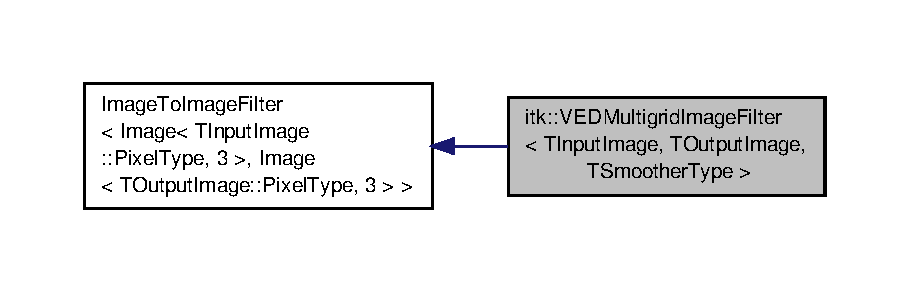
\includegraphics[width=350pt]{classitk_1_1_v_e_d_multigrid_image_filter__inherit__graph}
\end{center}
\end{figure}


Collaboration diagram for itk\-:\-:V\-E\-D\-Multigrid\-Image\-Filter$<$ T\-Input\-Image, T\-Output\-Image, T\-Smoother\-Type $>$\-:
\nopagebreak
\begin{figure}[H]
\begin{center}
\leavevmode
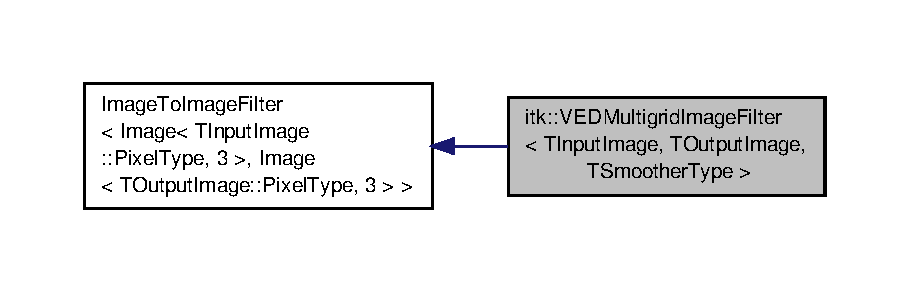
\includegraphics[width=350pt]{classitk_1_1_v_e_d_multigrid_image_filter__coll__graph}
\end{center}
\end{figure}
\subsection*{Public Types}
\begin{DoxyCompactItemize}
\item 
typedef \hyperlink{classitk_1_1_v_e_d_multigrid_image_filter}{V\-E\-D\-Multigrid\-Image\-Filter} \hyperlink{classitk_1_1_v_e_d_multigrid_image_filter_a4e79c36d98793a398699ebf672d78762}{Self}
\item 
\hypertarget{classitk_1_1_v_e_d_multigrid_image_filter_a2c8aaf15075eb5b1471b156af0a08328}{typedef \hyperlink{class_image_to_image_filter}{Image\-To\-Image\-Filter}\\*
$<$ T\-Input\-Image, T\-Output\-Image $>$ {\bfseries Super\-Class}}\label{classitk_1_1_v_e_d_multigrid_image_filter_a2c8aaf15075eb5b1471b156af0a08328}

\item 
\hypertarget{classitk_1_1_v_e_d_multigrid_image_filter_afb9004352b203770df9249e506eda3cf}{typedef Smart\-Pointer$<$ \hyperlink{classitk_1_1_v_e_d_multigrid_image_filter_a4e79c36d98793a398699ebf672d78762}{Self} $>$ {\bfseries Pointer}}\label{classitk_1_1_v_e_d_multigrid_image_filter_afb9004352b203770df9249e506eda3cf}

\item 
\hypertarget{classitk_1_1_v_e_d_multigrid_image_filter_a0f1b52d57947e4d1fa9e23f1b4bc5ad3}{typedef Smart\-Pointer$<$ const \hyperlink{classitk_1_1_v_e_d_multigrid_image_filter_a4e79c36d98793a398699ebf672d78762}{Self} $>$ {\bfseries Const\-Pointer}}\label{classitk_1_1_v_e_d_multigrid_image_filter_a0f1b52d57947e4d1fa9e23f1b4bc5ad3}

\item 
\hypertarget{classitk_1_1_v_e_d_multigrid_image_filter_a86196537f4b1494ef84c83cf1ea966d5}{typedef T\-Input\-Image {\bfseries Input\-Image\-Type}}\label{classitk_1_1_v_e_d_multigrid_image_filter_a86196537f4b1494ef84c83cf1ea966d5}

\item 
\hypertarget{classitk_1_1_v_e_d_multigrid_image_filter_a43db82edf24ce3e881142d94b060c0c2}{typedef T\-Input\-Image\-::\-Pixel\-Type {\bfseries Input\-Pixel\-Type}}\label{classitk_1_1_v_e_d_multigrid_image_filter_a43db82edf24ce3e881142d94b060c0c2}

\item 
\hypertarget{classitk_1_1_v_e_d_multigrid_image_filter_ab44f3479119b729cb49ce3f1765c0708}{typedef T\-Output\-Image {\bfseries Output\-Image\-Type}}\label{classitk_1_1_v_e_d_multigrid_image_filter_ab44f3479119b729cb49ce3f1765c0708}

\item 
\hypertarget{classitk_1_1_v_e_d_multigrid_image_filter_a0ca4057a987d16d007b8ba81777a0478}{typedef T\-Output\-Image\-::\-Pixel\-Type {\bfseries Output\-Pixel\-Type}}\label{classitk_1_1_v_e_d_multigrid_image_filter_a0ca4057a987d16d007b8ba81777a0478}

\item 
\hypertarget{classitk_1_1_v_e_d_multigrid_image_filter_afc4a041c3cb9883fbdff62fbeaf397b8}{typedef double {\bfseries Internal\-Pixel\-Type}}\label{classitk_1_1_v_e_d_multigrid_image_filter_afc4a041c3cb9883fbdff62fbeaf397b8}

\item 
\hypertarget{classitk_1_1_v_e_d_multigrid_image_filter_a9af7293ad6affb1fb33069e7fe4e58e0}{typedef \hyperlink{class_image}{Image}\\*
$<$ Internal\-Pixel\-Type, 3 $>$ {\bfseries Internal\-Image\-Type}}\label{classitk_1_1_v_e_d_multigrid_image_filter_a9af7293ad6affb1fb33069e7fe4e58e0}

\item 
\hypertarget{classitk_1_1_v_e_d_multigrid_image_filter_a63b34df60b6eeb9d1e9a0c7702d689b8}{typedef \hyperlink{class_image}{Image}\\*
$<$ Symmetric\-Second\-Rank\-Tensor\\*
$<$ Internal\-Pixel\-Type, 3 $>$, 3 $>$ {\bfseries Tensor\-Image\-Type}}\label{classitk_1_1_v_e_d_multigrid_image_filter_a63b34df60b6eeb9d1e9a0c7702d689b8}

\item 
\hypertarget{classitk_1_1_v_e_d_multigrid_image_filter_a63a3fe60f6b4bf4485e3474ef54a03d2}{typedef Internal\-Pixel\-Type {\bfseries Precision}}\label{classitk_1_1_v_e_d_multigrid_image_filter_a63a3fe60f6b4bf4485e3474ef54a03d2}

\item 
\hypertarget{classitk_1_1_v_e_d_multigrid_image_filter_a7832aaee343deb63ab4ca732964ef453}{typedef Image\-Region$<$ 3 $>$ {\bfseries Image\-Region\-Type}}\label{classitk_1_1_v_e_d_multigrid_image_filter_a7832aaee343deb63ab4ca732964ef453}

\item 
\hypertarget{classitk_1_1_v_e_d_multigrid_image_filter_a299326786f185c91052a6fc2e1725d67}{typedef Fixed\-Array$<$ Precision, 3 $>$ {\bfseries Vector\-Type}}\label{classitk_1_1_v_e_d_multigrid_image_filter_a299326786f185c91052a6fc2e1725d67}

\item 
\hypertarget{classitk_1_1_v_e_d_multigrid_image_filter_a2926b7cbac14c5aa3d0a6fcb810d2fb4}{typedef \hyperlink{class_image}{Image}$<$ Vector\-Type, 3 $>$ {\bfseries Vector\-Image\-Type}}\label{classitk_1_1_v_e_d_multigrid_image_filter_a2926b7cbac14c5aa3d0a6fcb810d2fb4}

\item 
\hypertarget{classitk_1_1_v_e_d_multigrid_image_filter_a2bb0bd96e8015b5411cf8ea427015623}{typedef Matrix$<$ Precision, 3, 3 $>$ {\bfseries Matrix\-Type}}\label{classitk_1_1_v_e_d_multigrid_image_filter_a2bb0bd96e8015b5411cf8ea427015623}

\item 
\hypertarget{classitk_1_1_v_e_d_multigrid_image_filter_a6246de6b8751b51198accf31b3809428}{typedef \hyperlink{class_image}{Image}$<$ Matrix\-Type, 3 $>$ {\bfseries Matrix\-Image\-Type}}\label{classitk_1_1_v_e_d_multigrid_image_filter_a6246de6b8751b51198accf31b3809428}

\item 
\hypertarget{classitk_1_1_v_e_d_multigrid_image_filter_a85d338d00e13192258181aa2af45d331}{typedef \\*
\hyperlink{classitk_1_1_multigrid_anisotropic_diffusion_image_filter}{Multigrid\-Anisotropic\-Diffusion\-Image\-Filter}\\*
$<$ \hyperlink{class_image}{Internal\-Image\-Type}, \\*
\hyperlink{class_image}{Internal\-Image\-Type}, \\*
T\-Smoother\-Type $>$ {\bfseries M\-A\-D\-Filter\-Type}}\label{classitk_1_1_v_e_d_multigrid_image_filter_a85d338d00e13192258181aa2af45d331}

\item 
\hypertarget{classitk_1_1_v_e_d_multigrid_image_filter_a266c29175fe64dfb7020ecac3f29c9a6}{typedef \\*
M\-A\-D\-Filter\-Type\-::\-Coarse\-Grid\-Operator\-Type {\bfseries Coarse\-Grid\-Operator\-Type}}\label{classitk_1_1_v_e_d_multigrid_image_filter_a266c29175fe64dfb7020ecac3f29c9a6}

\item 
\hypertarget{classitk_1_1_v_e_d_multigrid_image_filter_a18f9a5f1db18950100ab4805661d9634}{typedef M\-A\-D\-Filter\-Type\-::\-Cycle\-Type {\bfseries Cycle\-Type}}\label{classitk_1_1_v_e_d_multigrid_image_filter_a18f9a5f1db18950100ab4805661d9634}

\end{DoxyCompactItemize}
\subsection*{Public Member Functions}
\begin{DoxyCompactItemize}
\item 
\hyperlink{classitk_1_1_v_e_d_multigrid_image_filter_a20bd54f37685bf1e56408c0391429522}{itk\-New\-Macro} (\hyperlink{classitk_1_1_v_e_d_multigrid_image_filter_a4e79c36d98793a398699ebf672d78762}{Self})
\item 
\hyperlink{classitk_1_1_v_e_d_multigrid_image_filter_a36bb17743677b7b128f4a2daf901d451}{itk\-Type\-Macro} (\hyperlink{classitk_1_1_v_e_d_multigrid_image_filter}{V\-E\-D\-Multigrid\-Image\-Filter}, \hyperlink{class_image_to_image_filter}{Image\-To\-Image\-Filter})
\item 
\hyperlink{classitk_1_1_v_e_d_multigrid_image_filter_aa775d9c3a2d15a5ea172b00dd4958a10}{itk\-Set\-Macro} (Alpha, Precision)
\item 
\hypertarget{classitk_1_1_v_e_d_multigrid_image_filter_a996fbccff298c686a669c10779cc2239}{{\bfseries itk\-Set\-Macro} (Beta, Precision)}\label{classitk_1_1_v_e_d_multigrid_image_filter_a996fbccff298c686a669c10779cc2239}

\item 
\hypertarget{classitk_1_1_v_e_d_multigrid_image_filter_a692d8a063982214189d7f34f0d539318}{{\bfseries itk\-Set\-Macro} (Gamma, Precision)}\label{classitk_1_1_v_e_d_multigrid_image_filter_a692d8a063982214189d7f34f0d539318}

\item 
\hypertarget{classitk_1_1_v_e_d_multigrid_image_filter_aca52dec3af2a2383ef7d8027ea73f5be}{{\bfseries itk\-Set\-Macro} (Epsilon, Precision)}\label{classitk_1_1_v_e_d_multigrid_image_filter_aca52dec3af2a2383ef7d8027ea73f5be}

\item 
\hypertarget{classitk_1_1_v_e_d_multigrid_image_filter_ab8cf92c710c43f11cd587adefd295d8e}{{\bfseries itk\-Set\-Macro} (Omega, Precision)}\label{classitk_1_1_v_e_d_multigrid_image_filter_ab8cf92c710c43f11cd587adefd295d8e}

\item 
\hypertarget{classitk_1_1_v_e_d_multigrid_image_filter_ac2f07dc67d0020cb64e44bdcffb1e2a7}{{\bfseries itk\-Set\-Macro} (Sensitivity, Precision)}\label{classitk_1_1_v_e_d_multigrid_image_filter_ac2f07dc67d0020cb64e44bdcffb1e2a7}

\item 
\hypertarget{classitk_1_1_v_e_d_multigrid_image_filter_a1ddf29473bfa840ffbba4ab726c7921d}{{\bfseries itk\-Set\-Macro} (Scales, std\-::vector$<$ Precision $>$)}\label{classitk_1_1_v_e_d_multigrid_image_filter_a1ddf29473bfa840ffbba4ab726c7921d}

\item 
\hypertarget{classitk_1_1_v_e_d_multigrid_image_filter_a08bf9b177cd9ac26845da6aa995ffc6a}{{\bfseries itk\-Set\-Macro} (Iterations, unsigned int)}\label{classitk_1_1_v_e_d_multigrid_image_filter_a08bf9b177cd9ac26845da6aa995ffc6a}

\item 
\hypertarget{classitk_1_1_v_e_d_multigrid_image_filter_a71691b1fa6b5ea9490e2cb509ba38bf7}{{\bfseries itk\-Set\-Macro} (Diffusion\-Iterations, unsigned int)}\label{classitk_1_1_v_e_d_multigrid_image_filter_a71691b1fa6b5ea9490e2cb509ba38bf7}

\item 
\hyperlink{classitk_1_1_v_e_d_multigrid_image_filter_aab2fb17d7dfabd19af4009ddea3f67f1}{itk\-Set\-Macro} (Coarse\-Grid\-Operator, Coarse\-Grid\-Operator\-Type)
\item 
\hypertarget{classitk_1_1_v_e_d_multigrid_image_filter_aff8194cac314541f0e98d7adb876ffad}{{\bfseries itk\-Set\-Macro} (Cycle, Cycle\-Type)}\label{classitk_1_1_v_e_d_multigrid_image_filter_aff8194cac314541f0e98d7adb876ffad}

\item 
\hypertarget{classitk_1_1_v_e_d_multigrid_image_filter_a832d02ed6da4e69a9e8aa8f1f7a8f541}{{\bfseries itk\-Set\-Macro} (Time\-Step, Precision)}\label{classitk_1_1_v_e_d_multigrid_image_filter_a832d02ed6da4e69a9e8aa8f1f7a8f541}

\item 
\hypertarget{classitk_1_1_v_e_d_multigrid_image_filter_a8a980466133156d782b1db394f595730}{{\bfseries itk\-Set\-Macro} (Tolerance, Precision)}\label{classitk_1_1_v_e_d_multigrid_image_filter_a8a980466133156d782b1db394f595730}

\item 
\hypertarget{classitk_1_1_v_e_d_multigrid_image_filter_abe42c9105de2a52b7b8912afd5cf8136}{{\bfseries itk\-Set\-Macro} (Diffusion\-Iterations\-Per\-Grid, unsigned int)}\label{classitk_1_1_v_e_d_multigrid_image_filter_abe42c9105de2a52b7b8912afd5cf8136}

\item 
\hyperlink{classitk_1_1_v_e_d_multigrid_image_filter_aa483bcbaf19bd8b9128e143158238aca}{itk\-Set\-Macro} (Verbose, bool)
\item 
void \hyperlink{classitk_1_1_v_e_d_multigrid_image_filter_aa6accfcc728e7553c92c8a551c30ab11}{Set\-Input} (const Input\-Image\-Type $\ast$input\-Image)
\end{DoxyCompactItemize}
\subsection*{Protected Member Functions}
\begin{DoxyCompactItemize}
\item 
\hyperlink{classitk_1_1_v_e_d_multigrid_image_filter_a5d015ab30d15fe78c39e532ec69188d9}{V\-E\-D\-Multigrid\-Image\-Filter} ()
\item 
\hyperlink{classitk_1_1_v_e_d_multigrid_image_filter_ac614b2d03c2ce4f6f7403f6459926386}{$\sim$\-V\-E\-D\-Multigrid\-Image\-Filter} ()
\item 
virtual void \hyperlink{classitk_1_1_v_e_d_multigrid_image_filter_a90c199154c057be714f541c2cdd4c3f2}{Generate\-Data} ()
\end{DoxyCompactItemize}


\subsection{Detailed Description}
\subsubsection*{template$<$class T\-Input\-Image, class T\-Output\-Image, class T\-Smoother\-Type = mad\-::\-Multigrid\-Gauss\-Seidel\-Smoother$<$ T\-Input\-Image\-::\-Image\-Dimension $>$$>$class itk\-::\-V\-E\-D\-Multigrid\-Image\-Filter$<$ T\-Input\-Image, T\-Output\-Image, T\-Smoother\-Type $>$}

Implementation of the V\-E\-D method by Manniesing, which internally uses \hyperlink{classitk_1_1_multigrid_anisotropic_diffusion_image_filter}{Multigrid\-Anisotropic\-Diffusion\-Image\-Filter} for the diffusion steps. 

Reference for the algorithm\-: R Manniesing, M\-A Viergever, W\-J Niessen, {\itshape Vessel enhancing diffusion\-: A scale space representation of vessel structures}, Medical \hyperlink{class_image}{Image} Analysis 10(6), 815-\/825.

\begin{DoxyAuthor}{Author}
Antonello Gerbi 
\end{DoxyAuthor}


Definition at line 47 of file itk\-V\-E\-D\-Multigrid\-Image\-Filter.\-h.



\subsection{Member Typedef Documentation}
\hypertarget{classitk_1_1_v_e_d_multigrid_image_filter_a4e79c36d98793a398699ebf672d78762}{\index{itk\-::\-V\-E\-D\-Multigrid\-Image\-Filter@{itk\-::\-V\-E\-D\-Multigrid\-Image\-Filter}!Self@{Self}}
\index{Self@{Self}!itk::VEDMultigridImageFilter@{itk\-::\-V\-E\-D\-Multigrid\-Image\-Filter}}
\subsubsection[{Self}]{\setlength{\rightskip}{0pt plus 5cm}template$<$class T\-Input\-Image, class T\-Output\-Image, class T\-Smoother\-Type = mad\-::\-Multigrid\-Gauss\-Seidel\-Smoother$<$ T\-Input\-Image\-::\-Image\-Dimension $>$$>$ typedef {\bf V\-E\-D\-Multigrid\-Image\-Filter} {\bf itk\-::\-V\-E\-D\-Multigrid\-Image\-Filter}$<$ T\-Input\-Image, T\-Output\-Image, T\-Smoother\-Type $>$\-::{\bf Self}}}\label{classitk_1_1_v_e_d_multigrid_image_filter_a4e79c36d98793a398699ebf672d78762}
Standard and useful class typedefs. 

Definition at line 53 of file itk\-V\-E\-D\-Multigrid\-Image\-Filter.\-h.



\subsection{Constructor \& Destructor Documentation}
\hypertarget{classitk_1_1_v_e_d_multigrid_image_filter_a5d015ab30d15fe78c39e532ec69188d9}{\index{itk\-::\-V\-E\-D\-Multigrid\-Image\-Filter@{itk\-::\-V\-E\-D\-Multigrid\-Image\-Filter}!V\-E\-D\-Multigrid\-Image\-Filter@{V\-E\-D\-Multigrid\-Image\-Filter}}
\index{V\-E\-D\-Multigrid\-Image\-Filter@{V\-E\-D\-Multigrid\-Image\-Filter}!itk::VEDMultigridImageFilter@{itk\-::\-V\-E\-D\-Multigrid\-Image\-Filter}}
\subsubsection[{V\-E\-D\-Multigrid\-Image\-Filter}]{\setlength{\rightskip}{0pt plus 5cm}template$<$class T\-Input\-Image , class T\-Output\-Image , class T\-Smoother\-Type $>$ {\bf itk\-::\-V\-E\-D\-Multigrid\-Image\-Filter}$<$ T\-Input\-Image, T\-Output\-Image, T\-Smoother\-Type $>$\-::{\bf V\-E\-D\-Multigrid\-Image\-Filter} (
\begin{DoxyParamCaption}
{}
\end{DoxyParamCaption}
)\hspace{0.3cm}{\ttfamily [protected]}}}\label{classitk_1_1_v_e_d_multigrid_image_filter_a5d015ab30d15fe78c39e532ec69188d9}
Class constructor. 

Definition at line 45 of file itk\-V\-E\-D\-Multigrid\-Image\-Filter.\-hxx.

\hypertarget{classitk_1_1_v_e_d_multigrid_image_filter_ac614b2d03c2ce4f6f7403f6459926386}{\index{itk\-::\-V\-E\-D\-Multigrid\-Image\-Filter@{itk\-::\-V\-E\-D\-Multigrid\-Image\-Filter}!$\sim$\-V\-E\-D\-Multigrid\-Image\-Filter@{$\sim$\-V\-E\-D\-Multigrid\-Image\-Filter}}
\index{$\sim$\-V\-E\-D\-Multigrid\-Image\-Filter@{$\sim$\-V\-E\-D\-Multigrid\-Image\-Filter}!itk::VEDMultigridImageFilter@{itk\-::\-V\-E\-D\-Multigrid\-Image\-Filter}}
\subsubsection[{$\sim$\-V\-E\-D\-Multigrid\-Image\-Filter}]{\setlength{\rightskip}{0pt plus 5cm}template$<$class T\-Input\-Image , class T\-Output\-Image , class T\-Smoother\-Type $>$ {\bf itk\-::\-V\-E\-D\-Multigrid\-Image\-Filter}$<$ T\-Input\-Image, T\-Output\-Image, T\-Smoother\-Type $>$\-::$\sim${\bf V\-E\-D\-Multigrid\-Image\-Filter} (
\begin{DoxyParamCaption}
{}
\end{DoxyParamCaption}
)\hspace{0.3cm}{\ttfamily [protected]}}}\label{classitk_1_1_v_e_d_multigrid_image_filter_ac614b2d03c2ce4f6f7403f6459926386}
Class destructor. 

Definition at line 420 of file itk\-V\-E\-D\-Multigrid\-Image\-Filter.\-hxx.



\subsection{Member Function Documentation}
\hypertarget{classitk_1_1_v_e_d_multigrid_image_filter_a90c199154c057be714f541c2cdd4c3f2}{\index{itk\-::\-V\-E\-D\-Multigrid\-Image\-Filter@{itk\-::\-V\-E\-D\-Multigrid\-Image\-Filter}!Generate\-Data@{Generate\-Data}}
\index{Generate\-Data@{Generate\-Data}!itk::VEDMultigridImageFilter@{itk\-::\-V\-E\-D\-Multigrid\-Image\-Filter}}
\subsubsection[{Generate\-Data}]{\setlength{\rightskip}{0pt plus 5cm}template$<$class T\-Input\-Image , class T\-Output\-Image , class T\-Smoother\-Type $>$ void {\bf itk\-::\-V\-E\-D\-Multigrid\-Image\-Filter}$<$ T\-Input\-Image, T\-Output\-Image, T\-Smoother\-Type $>$\-::Generate\-Data (
\begin{DoxyParamCaption}
{}
\end{DoxyParamCaption}
)\hspace{0.3cm}{\ttfamily [protected]}, {\ttfamily [virtual]}}}\label{classitk_1_1_v_e_d_multigrid_image_filter_a90c199154c057be714f541c2cdd4c3f2}
Generates the output. 

Definition at line 78 of file itk\-V\-E\-D\-Multigrid\-Image\-Filter.\-hxx.

\hypertarget{classitk_1_1_v_e_d_multigrid_image_filter_a20bd54f37685bf1e56408c0391429522}{\index{itk\-::\-V\-E\-D\-Multigrid\-Image\-Filter@{itk\-::\-V\-E\-D\-Multigrid\-Image\-Filter}!itk\-New\-Macro@{itk\-New\-Macro}}
\index{itk\-New\-Macro@{itk\-New\-Macro}!itk::VEDMultigridImageFilter@{itk\-::\-V\-E\-D\-Multigrid\-Image\-Filter}}
\subsubsection[{itk\-New\-Macro}]{\setlength{\rightskip}{0pt plus 5cm}template$<$class T\-Input\-Image, class T\-Output\-Image, class T\-Smoother\-Type = mad\-::\-Multigrid\-Gauss\-Seidel\-Smoother$<$ T\-Input\-Image\-::\-Image\-Dimension $>$$>$ {\bf itk\-::\-V\-E\-D\-Multigrid\-Image\-Filter}$<$ T\-Input\-Image, T\-Output\-Image, T\-Smoother\-Type $>$\-::itk\-New\-Macro (
\begin{DoxyParamCaption}
\item[{{\bf Self}}]{}
\end{DoxyParamCaption}
)}}\label{classitk_1_1_v_e_d_multigrid_image_filter_a20bd54f37685bf1e56408c0391429522}
Method for creation through the object factory. \hypertarget{classitk_1_1_v_e_d_multigrid_image_filter_aa775d9c3a2d15a5ea172b00dd4958a10}{\index{itk\-::\-V\-E\-D\-Multigrid\-Image\-Filter@{itk\-::\-V\-E\-D\-Multigrid\-Image\-Filter}!itk\-Set\-Macro@{itk\-Set\-Macro}}
\index{itk\-Set\-Macro@{itk\-Set\-Macro}!itk::VEDMultigridImageFilter@{itk\-::\-V\-E\-D\-Multigrid\-Image\-Filter}}
\subsubsection[{itk\-Set\-Macro}]{\setlength{\rightskip}{0pt plus 5cm}template$<$class T\-Input\-Image, class T\-Output\-Image, class T\-Smoother\-Type = mad\-::\-Multigrid\-Gauss\-Seidel\-Smoother$<$ T\-Input\-Image\-::\-Image\-Dimension $>$$>$ {\bf itk\-::\-V\-E\-D\-Multigrid\-Image\-Filter}$<$ T\-Input\-Image, T\-Output\-Image, T\-Smoother\-Type $>$\-::itk\-Set\-Macro (
\begin{DoxyParamCaption}
\item[{Alpha}]{, }
\item[{Precision}]{}
\end{DoxyParamCaption}
)}}\label{classitk_1_1_v_e_d_multigrid_image_filter_aa775d9c3a2d15a5ea172b00dd4958a10}
Setters for V\-E\-D parameters. \hypertarget{classitk_1_1_v_e_d_multigrid_image_filter_aab2fb17d7dfabd19af4009ddea3f67f1}{\index{itk\-::\-V\-E\-D\-Multigrid\-Image\-Filter@{itk\-::\-V\-E\-D\-Multigrid\-Image\-Filter}!itk\-Set\-Macro@{itk\-Set\-Macro}}
\index{itk\-Set\-Macro@{itk\-Set\-Macro}!itk::VEDMultigridImageFilter@{itk\-::\-V\-E\-D\-Multigrid\-Image\-Filter}}
\subsubsection[{itk\-Set\-Macro}]{\setlength{\rightskip}{0pt plus 5cm}template$<$class T\-Input\-Image, class T\-Output\-Image, class T\-Smoother\-Type = mad\-::\-Multigrid\-Gauss\-Seidel\-Smoother$<$ T\-Input\-Image\-::\-Image\-Dimension $>$$>$ {\bf itk\-::\-V\-E\-D\-Multigrid\-Image\-Filter}$<$ T\-Input\-Image, T\-Output\-Image, T\-Smoother\-Type $>$\-::itk\-Set\-Macro (
\begin{DoxyParamCaption}
\item[{Coarse\-Grid\-Operator}]{, }
\item[{Coarse\-Grid\-Operator\-Type}]{}
\end{DoxyParamCaption}
)}}\label{classitk_1_1_v_e_d_multigrid_image_filter_aab2fb17d7dfabd19af4009ddea3f67f1}
Setters for M\-A\-D parameters. \hypertarget{classitk_1_1_v_e_d_multigrid_image_filter_aa483bcbaf19bd8b9128e143158238aca}{\index{itk\-::\-V\-E\-D\-Multigrid\-Image\-Filter@{itk\-::\-V\-E\-D\-Multigrid\-Image\-Filter}!itk\-Set\-Macro@{itk\-Set\-Macro}}
\index{itk\-Set\-Macro@{itk\-Set\-Macro}!itk::VEDMultigridImageFilter@{itk\-::\-V\-E\-D\-Multigrid\-Image\-Filter}}
\subsubsection[{itk\-Set\-Macro}]{\setlength{\rightskip}{0pt plus 5cm}template$<$class T\-Input\-Image, class T\-Output\-Image, class T\-Smoother\-Type = mad\-::\-Multigrid\-Gauss\-Seidel\-Smoother$<$ T\-Input\-Image\-::\-Image\-Dimension $>$$>$ {\bf itk\-::\-V\-E\-D\-Multigrid\-Image\-Filter}$<$ T\-Input\-Image, T\-Output\-Image, T\-Smoother\-Type $>$\-::itk\-Set\-Macro (
\begin{DoxyParamCaption}
\item[{Verbose}]{, }
\item[{bool}]{}
\end{DoxyParamCaption}
)}}\label{classitk_1_1_v_e_d_multigrid_image_filter_aa483bcbaf19bd8b9128e143158238aca}
Sets wether the filter should produce textual output containing informations on the current status. \hypertarget{classitk_1_1_v_e_d_multigrid_image_filter_a36bb17743677b7b128f4a2daf901d451}{\index{itk\-::\-V\-E\-D\-Multigrid\-Image\-Filter@{itk\-::\-V\-E\-D\-Multigrid\-Image\-Filter}!itk\-Type\-Macro@{itk\-Type\-Macro}}
\index{itk\-Type\-Macro@{itk\-Type\-Macro}!itk::VEDMultigridImageFilter@{itk\-::\-V\-E\-D\-Multigrid\-Image\-Filter}}
\subsubsection[{itk\-Type\-Macro}]{\setlength{\rightskip}{0pt plus 5cm}template$<$class T\-Input\-Image, class T\-Output\-Image, class T\-Smoother\-Type = mad\-::\-Multigrid\-Gauss\-Seidel\-Smoother$<$ T\-Input\-Image\-::\-Image\-Dimension $>$$>$ {\bf itk\-::\-V\-E\-D\-Multigrid\-Image\-Filter}$<$ T\-Input\-Image, T\-Output\-Image, T\-Smoother\-Type $>$\-::itk\-Type\-Macro (
\begin{DoxyParamCaption}
\item[{{\bf V\-E\-D\-Multigrid\-Image\-Filter}$<$ T\-Input\-Image, T\-Output\-Image, T\-Smoother\-Type $>$}]{, }
\item[{{\bf Image\-To\-Image\-Filter}}]{}
\end{DoxyParamCaption}
)}}\label{classitk_1_1_v_e_d_multigrid_image_filter_a36bb17743677b7b128f4a2daf901d451}
Run-\/time type information (and related methods). \hypertarget{classitk_1_1_v_e_d_multigrid_image_filter_aa6accfcc728e7553c92c8a551c30ab11}{\index{itk\-::\-V\-E\-D\-Multigrid\-Image\-Filter@{itk\-::\-V\-E\-D\-Multigrid\-Image\-Filter}!Set\-Input@{Set\-Input}}
\index{Set\-Input@{Set\-Input}!itk::VEDMultigridImageFilter@{itk\-::\-V\-E\-D\-Multigrid\-Image\-Filter}}
\subsubsection[{Set\-Input}]{\setlength{\rightskip}{0pt plus 5cm}template$<$class T\-Input\-Image , class T\-Output\-Image , class T\-Smoother\-Type $>$ void {\bf itk\-::\-V\-E\-D\-Multigrid\-Image\-Filter}$<$ T\-Input\-Image, T\-Output\-Image, T\-Smoother\-Type $>$\-::Set\-Input (
\begin{DoxyParamCaption}
\item[{const Input\-Image\-Type $\ast$}]{input\-Image}
\end{DoxyParamCaption}
)}}\label{classitk_1_1_v_e_d_multigrid_image_filter_aa6accfcc728e7553c92c8a551c30ab11}
Input image setter. 

Definition at line 35 of file itk\-V\-E\-D\-Multigrid\-Image\-Filter.\-hxx.



The documentation for this class was generated from the following files\-:\begin{DoxyCompactItemize}
\item 
itk\-V\-E\-D\-Multigrid\-Image\-Filter.\-h\item 
itk\-V\-E\-D\-Multigrid\-Image\-Filter.\-hxx\end{DoxyCompactItemize}

\printindex
\end{document}
